\documentclass[twoside]{book}

% Packages required by doxygen
\usepackage{fixltx2e}
\usepackage{calc}
\usepackage{doxygen}
\usepackage[export]{adjustbox} % also loads graphicx
\usepackage{graphicx}
\usepackage[utf8]{inputenc}
\usepackage{makeidx}
\usepackage{multicol}
\usepackage{multirow}
\PassOptionsToPackage{warn}{textcomp}
\usepackage{textcomp}
\usepackage[nointegrals]{wasysym}
\usepackage[table]{xcolor}

% Font selection
\usepackage[T1]{fontenc}
\usepackage[scaled=.90]{helvet}
\usepackage{courier}
\usepackage{amssymb}
\usepackage{sectsty}
\renewcommand{\familydefault}{\sfdefault}
\allsectionsfont{%
  \fontseries{bc}\selectfont%
  \color{darkgray}%
}
\renewcommand{\DoxyLabelFont}{%
  \fontseries{bc}\selectfont%
  \color{darkgray}%
}
\newcommand{\+}{\discretionary{\mbox{\scriptsize$\hookleftarrow$}}{}{}}

% Page & text layout
\usepackage{geometry}
\geometry{%
  a4paper,%
  top=2.5cm,%
  bottom=2.5cm,%
  left=2.5cm,%
  right=2.5cm%
}
\tolerance=750
\hfuzz=15pt
\hbadness=750
\setlength{\emergencystretch}{15pt}
\setlength{\parindent}{0cm}
\setlength{\parskip}{3ex plus 2ex minus 2ex}
\makeatletter
\renewcommand{\paragraph}{%
  \@startsection{paragraph}{4}{0ex}{-1.0ex}{1.0ex}{%
    \normalfont\normalsize\bfseries\SS@parafont%
  }%
}
\renewcommand{\subparagraph}{%
  \@startsection{subparagraph}{5}{0ex}{-1.0ex}{1.0ex}{%
    \normalfont\normalsize\bfseries\SS@subparafont%
  }%
}
\makeatother

% Headers & footers
\usepackage{fancyhdr}
\pagestyle{fancyplain}
\fancyhead[LE]{\fancyplain{}{\bfseries\thepage}}
\fancyhead[CE]{\fancyplain{}{}}
\fancyhead[RE]{\fancyplain{}{\bfseries\leftmark}}
\fancyhead[LO]{\fancyplain{}{\bfseries\rightmark}}
\fancyhead[CO]{\fancyplain{}{}}
\fancyhead[RO]{\fancyplain{}{\bfseries\thepage}}
\fancyfoot[LE]{\fancyplain{}{}}
\fancyfoot[CE]{\fancyplain{}{}}
\fancyfoot[RE]{\fancyplain{}{\bfseries\scriptsize Generated by Doxygen }}
\fancyfoot[LO]{\fancyplain{}{\bfseries\scriptsize Generated by Doxygen }}
\fancyfoot[CO]{\fancyplain{}{}}
\fancyfoot[RO]{\fancyplain{}{}}
\renewcommand{\footrulewidth}{0.4pt}
\renewcommand{\chaptermark}[1]{%
  \markboth{#1}{}%
}
\renewcommand{\sectionmark}[1]{%
  \markright{\thesection\ #1}%
}

% Indices & bibliography
\usepackage{natbib}
\usepackage[titles]{tocloft}
\setcounter{tocdepth}{3}
\setcounter{secnumdepth}{5}
\makeindex

% Hyperlinks (required, but should be loaded last)
\usepackage{ifpdf}
\ifpdf
  \usepackage[pdftex,pagebackref=true]{hyperref}
\else
  \usepackage[ps2pdf,pagebackref=true]{hyperref}
\fi
\hypersetup{%
  colorlinks=true,%
  linkcolor=blue,%
  citecolor=blue,%
  unicode%
}

% Custom commands
\newcommand{\clearemptydoublepage}{%
  \newpage{\pagestyle{empty}\cleardoublepage}%
}

\usepackage{caption}
\captionsetup{labelsep=space,justification=centering,font={bf},singlelinecheck=off,skip=4pt,position=top}

%===== C O N T E N T S =====

\begin{document}

% Titlepage & ToC
\hypersetup{pageanchor=false,
             bookmarksnumbered=true,
             pdfencoding=unicode
            }
\pagenumbering{alph}
\begin{titlepage}
\vspace*{7cm}
\begin{center}%
{\Large Cubium \\[1ex]\large 1.\+5 }\\
\vspace*{1cm}
{\large Generated by Doxygen 1.8.13}\\
\end{center}
\end{titlepage}
\clearemptydoublepage
\pagenumbering{roman}
\tableofcontents
\clearemptydoublepage
\pagenumbering{arabic}
\hypersetup{pageanchor=true}

%--- Begin generated contents ---
\chapter{Adafruit Python M\+C\+P9808}
\label{md_drivers_TempSensor_Adafruit_Python_MCP9808_README}
\Hypertarget{md_drivers_TempSensor_Adafruit_Python_MCP9808_README}
Python library for accessing the M\+C\+P9808 precision temperature sensor on a Raspberry Pi or Beaglebone Black.

Designed specifically to work with the Adafruit M\+C\+P9808 sensor -\/---$>$ \href{https://www.adafruit.com/product/1782}{\tt https\+://www.\+adafruit.\+com/product/1782}

To install, first make sure some dependencies are available by running the following commands (on a Raspbian or Beaglebone Black Debian install)\+:


\begin{DoxyCode}
sudo apt-get update
sudo apt-get install build-essential python-dev python-smbus
\end{DoxyCode}


Then download the library by clicking the download zip link to the right and unzip the archive somewhere on your Raspberry Pi or Beaglebone Black. Then execute the following command in the directory of the library\+:


\begin{DoxyCode}
sudo python setup.py install
\end{DoxyCode}


Make sure you have internet access on the device so it can download the required dependencies.

See examples of usage in the examples folder.

Adafruit invests time and resources providing this open source code, please support Adafruit and open-\/source hardware by purchasing products from Adafruit!

Written by Tony Di\+Cola for Adafruit Industries. M\+IT license, all text above must be included in any redistribution 
\chapter{Cubium}
\label{md_readme}
\Hypertarget{md_readme}
Cubium is a free and open-\/source flight software for Linux-\/based spacecraft systems. Cubium allows for a more standardized and streamlined method of handling systems with many connected components by providing the neccesarry network to allow automatic discovery and communication between components. Developed with undergraduate Cube\+Sat teams using systems such as Beaglebone Blacks and Raspberry Pis in mind, Cubium\textquotesingle{}s purpose is to lower the bar of entry for satellite development.

Cubium is designed using the Space Plug-\/and-\/play Architecture (S\+PA), a specification for a kind of modular satellite software architecture. It has a proven mission-\/success track record on Air Force and Space Dynamics Laboratory payloads.

For a fun introduction on the inner workings of Cubium, see \href{https://drive.google.com/file/d/0ByiGNyJUAlpISUo5WDFwSkh3YU0/view?usp=sharing}{\tt this illustrated writeup.}

For a very detailed look into the machinations of S\+PA in general, see \href{http://digitalcommons.usu.edu/etd/1422/}{\tt Jacob Holt Christensen\textquotesingle{}s dissertation.}

\subsection*{Project Status}


\begin{DoxyItemize}
\item {\bfseries Version Alpha 1.\+2.\+0}
\begin{DoxyItemize}
\item Support for sending strings between components
\end{DoxyItemize}
\item {\bfseries Version Alpha 1.\+1.\+0}
\begin{DoxyItemize}
\item Finalized architecture for software demo shown at Small\+Sat conference
\end{DoxyItemize}
\item {\bfseries Version Alpha 1.\+0.\+0}
\begin{DoxyItemize}
\item All necessary framework completed for support of basic component systems.
\end{DoxyItemize}
\item {\bfseries Version Alpha 0.\+0.\+6}
\begin{DoxyItemize}
\item Successful transmission of S\+PA messages across processes via socket communication
\end{DoxyItemize}
\item {\bfseries Version Alpha 0.\+0.\+5}
\begin{DoxyItemize}
\item Major backend refactoring of S\+PA Messages
\end{DoxyItemize}
\item {\bfseries Version Alpha 0.\+0.\+4}
\begin{DoxyItemize}
\item Added a basic subscription service
\begin{DoxyItemize}
\item Direct component-\/to-\/component subscription
\item Non-\/prioritized publishing
\end{DoxyItemize}
\item Improvements to message handling
\item Additional tests for components
\end{DoxyItemize}
\item {\bfseries Version Alpha 0.\+0.\+3}
\begin{DoxyItemize}
\item Basic implementations of\+:
\begin{DoxyItemize}
\item Local Spa\+Messages
\item Components
\item Local Subnet Manager
\end{DoxyItemize}
\end{DoxyItemize}
\item {\bfseries Version Alpha 0.\+0.\+2}
\begin{DoxyItemize}
\item Debian dev environment complete
\end{DoxyItemize}
\item {\bfseries Version Alpha 0.\+0.\+1}
\begin{DoxyItemize}
\item Planning A\+PI\textquotesingle{}s and project planning
\end{DoxyItemize}
\end{DoxyItemize}

\subsection*{Getting Started}

\subsubsection*{Developer Tools}

Cubium relies on a handful of developer tools. The following is a list of things we\textquotesingle{}ll be using\+:
\begin{DoxyItemize}
\item Vagrant -\/ Virtual development environment
\item Git -\/ Version control system
\item Google Test -\/ Unit testing framework
\item Doxygen -\/ Documentation generator
\item C\+Make -\/ Build system automation
\end{DoxyItemize}

\subsubsection*{Set up Vagrant}

Cubium uses Vagrant to create a development environment to match the devices that Cubium will run on. It also eliminiates \char`\"{}well, it works on my system\char`\"{} bugs.

{\bfseries For instructions on getting the dev environment up and running, see the \href{https://github.com/Cubium/Cubium/wiki/Setting-up-the-Cubium-Dev-Environment}{\tt wiki page}}

\subsubsection*{Build Project}

\paragraph*{TL;DR}


\begin{DoxyItemize}
\item Run C\+Make in project directory {\ttfamily cmake .}
\item Run generated makefile {\ttfamily make \mbox{[}optional-\/target\mbox{]}}
\end{DoxyItemize}

Cubium uses C\+Make for a build system. Makefiles are generally platform-\/dependent, so C\+Make generates a different Makefile for each system in order to allow for cross-\/plaform functionality.

\subsubsection*{Build Docs}

\paragraph*{TL;DR}


\begin{DoxyItemize}
\item Run Doxygen with project doxyfile {\ttfamily doxygen ./\+Doxyfile}
\item View your docs. They should now live in {\ttfamily docs/}
\end{DoxyItemize}

Cubium uses the documentation generator Doxygen to build documentation. Annotated source code is parsed by Doxygen to generate La\+TeX and H\+T\+ML files.

Doxygen is configured with a file titled {\ttfamily Doxyfile}.


\begin{DoxyItemize}
\item Build Documentation
\begin{DoxyItemize}
\item Invoke commandline tool
\begin{DoxyItemize}
\item {\ttfamily doxygen Doxyfile}
\end{DoxyItemize}
\end{DoxyItemize}
\end{DoxyItemize}

This will read all configuration options from the Doxyfile, find and parse the source code, and generate the documentation.

If the documentation is successfully built, there should be a new directory title {\ttfamily docs/} that should contain both H\+T\+ML and La\+TeX documentation.


\begin{DoxyItemize}
\item Read Docs
\begin{DoxyItemize}
\item Open up {\ttfamily docs/html/index.\+html} in your web browser to browse docs
\end{DoxyItemize}
\end{DoxyItemize}

\subsubsection*{Running Tests}

Cubium tests use the Google Test testing framework for unit testing. Test test test.
\begin{DoxyItemize}
\item To run test suite\+:
\begin{DoxyItemize}
\item Generate a makefile with C\+Make {\ttfamily cmake .}
\item Build tests with makefile {\ttfamily make run\+Tests}
\item Run test executable {\ttfamily ./run\+Tests}
\end{DoxyItemize}
\end{DoxyItemize}

\subsubsection*{Testing}

Cubium uses Google Test for unit testing and C\+Make for a build system. The short version of running tests is this\+:

Classes should be kept small and have functioning unit tests. When adding a new header file for a class, a header file of the same name should be added to the {\ttfamily test/} directory.

To add a new class to the project\+:
\begin{DoxyItemize}
\item Create header file {\ttfamily my\+\_\+class\+\_\+name.\+hpp} (File names should be snake case -\/ lowercase words seperated with underscores)
\begin{DoxyItemize}
\item Define class ```cpp \#ifndef M\+Y\+\_\+\+C\+L\+A\+S\+S\+\_\+\+N\+A\+M\+E\+\_\+\+H\+PP \#define M\+Y\+\_\+\+C\+L\+A\+S\+S\+\_\+\+N\+A\+M\+E\+\_\+\+H\+PP class My\+Class\+Name\{\}; \#endif ```
\begin{DoxyItemize}
\item Must have include guards
\item Class name should be Upper\+Camel\+Case, where each first letter of a words is capitalized. Including the first word.
\end{DoxyItemize}
\end{DoxyItemize}
\item Add new testing file {\ttfamily test/my\+\_\+class\+\_\+name.\+hpp}
\item Write tests for your class ```cpp \#include \char`\"{}../path/to/my\+\_\+class\+\_\+name.\+hpp\char`\"{}

T\+E\+S\+T(\+My\+Class\+Name, my\+Method)\{ My\+Class\+Name my\+Class; E\+X\+P\+E\+C\+T\+\_\+\+EQ(my\+Class.\+my\+Method(),0); \} ```
\begin{DoxyItemize}
\item Be sure to include class header in test file
\end{DoxyItemize}
\item Include your test header in main test file
\begin{DoxyItemize}
\item Open {\ttfamily test/gtest\+\_\+main.\+cpp}
\item Include your new test header file
\end{DoxyItemize}
\item Hooray! Now you can run your tests! \+:D
\end{DoxyItemize}

\subsubsection*{Documentation}

Cubium uses Doxygen to build documentation from source code. This means that one can add comments with a special format in the code so that Doxygen may build pretty H\+T\+ML docs that can be referenced by all other developers and users.

Here is an example of what this might look like to document a function. 
\begin{DoxyCode}

\textcolor{keywordtype}{bool} example(\textcolor{keywordtype}{int} myParam)\{\textcolor{keywordflow}{return} \textcolor{keyword}{true};\}
\end{DoxyCode}
 
\chapter{Namespace Index}
\section{Namespace List}
Here is a list of all namespaces with brief descriptions\+:\begin{DoxyCompactList}
\item\contentsline{section}{\hyperlink{namespaceAdafruit__MCP9808}{Adafruit\+\_\+\+M\+C\+P9808} }{\pageref{namespaceAdafruit__MCP9808}}{}
\item\contentsline{section}{\hyperlink{namespaceAdafruit__MCP9808_1_1MCP9808}{Adafruit\+\_\+\+M\+C\+P9808.\+M\+C\+P9808} }{\pageref{namespaceAdafruit__MCP9808_1_1MCP9808}}{}
\item\contentsline{section}{\hyperlink{namespaceez__setup}{ez\+\_\+setup} }{\pageref{namespaceez__setup}}{}
\item\contentsline{section}{\hyperlink{namespacesetup}{setup} }{\pageref{namespacesetup}}{}
\item\contentsline{section}{\hyperlink{namespacesimpletest}{simpletest} }{\pageref{namespacesimpletest}}{}
\end{DoxyCompactList}

\chapter{Hierarchical Index}
\section{Class Hierarchy}
This inheritance list is sorted roughly, but not completely, alphabetically\+:\begin{DoxyCompactList}
\item \contentsline{section}{Component\+Info}{\pageref{structComponentInfo}}{}
\item \contentsline{section}{Component\+List}{\pageref{classComponentList}}{}
\item \contentsline{section}{cubium\+Client\+Socket\+\_\+t}{\pageref{structcubiumClientSocket__t}}{}
\item \contentsline{section}{cubium\+Server\+Socket\+\_\+t}{\pageref{structcubiumServerSocket__t}}{}
\item enable\+\_\+shared\+\_\+from\+\_\+this\begin{DoxyCompactList}
\item \contentsline{section}{Component}{\pageref{classComponent}}{}
\begin{DoxyCompactList}
\item \contentsline{section}{C\+O\+M\+P\+\_\+\+N\+A\+ME}{\pageref{classCOMP__NAME}}{}
\end{DoxyCompactList}
\item \contentsline{section}{Local\+Subnet\+Manager}{\pageref{classLocalSubnetManager}}{}
\end{DoxyCompactList}
\item \contentsline{section}{Local\+Ack}{\pageref{structLocalAck}}{}
\item \contentsline{section}{Local\+Hello}{\pageref{structLocalHello}}{}
\item \contentsline{section}{Local\+Spa\+Message}{\pageref{structLocalSpaMessage}}{}
\item \contentsline{section}{Logical\+Address}{\pageref{structLogicalAddress}}{}
\item \contentsline{section}{Logical\+Address\+Compare}{\pageref{structLogicalAddressCompare}}{}
\item object\begin{DoxyCompactList}
\item \contentsline{section}{Adafruit\+\_\+\+M\+C\+P9808.\+M\+C\+P9808.\+M\+C\+P9808}{\pageref{classAdafruit__MCP9808_1_1MCP9808_1_1MCP9808}}{}
\end{DoxyCompactList}
\item \contentsline{section}{Physical\+Communicator}{\pageref{classPhysicalCommunicator}}{}
\begin{DoxyCompactList}
\item \contentsline{section}{Local\+Communicator}{\pageref{classLocalCommunicator}}{}
\end{DoxyCompactList}
\item \contentsline{section}{Routing\+Table$<$ T $>$}{\pageref{classRoutingTable}}{}
\item \contentsline{section}{Spa\+Communicator}{\pageref{classSpaCommunicator}}{}
\item \contentsline{section}{Spa\+Courier}{\pageref{structSpaCourier}}{}
\item \contentsline{section}{Spa\+Data$<$ T $>$}{\pageref{structSpaData}}{}
\item \contentsline{section}{Spa\+Header}{\pageref{structSpaHeader}}{}
\item \contentsline{section}{Spa\+Local\+Header}{\pageref{structSpaLocalHeader}}{}
\item \contentsline{section}{Spa\+Message}{\pageref{structSpaMessage}}{}
\item \contentsline{section}{Subnet\+Manager}{\pageref{classSubnetManager}}{}
\begin{DoxyCompactList}
\item \contentsline{section}{Local\+Subnet\+Manager}{\pageref{classLocalSubnetManager}}{}
\end{DoxyCompactList}
\item \contentsline{section}{Subscriber}{\pageref{structSubscriber}}{}
\item \contentsline{section}{Subscription\+Reply}{\pageref{structSubscriptionReply}}{}
\item \contentsline{section}{Subscription\+Request}{\pageref{structSubscriptionRequest}}{}
\end{DoxyCompactList}

\chapter{Class Index}
\section{Class List}
Here are the classes, structs, unions and interfaces with brief descriptions\+:\begin{DoxyCompactList}
\item\contentsline{section}{\hyperlink{classCOMP__NAME}{C\+O\+M\+P\+\_\+\+N\+A\+ME} }{\pageref{classCOMP__NAME}}{}
\item\contentsline{section}{\hyperlink{classComponent}{Component} }{\pageref{classComponent}}{}
\item\contentsline{section}{\hyperlink{structComponentInfo}{Component\+Info} }{\pageref{structComponentInfo}}{}
\item\contentsline{section}{\hyperlink{classComponentList}{Component\+List} }{\pageref{classComponentList}}{}
\item\contentsline{section}{\hyperlink{structcubiumClientSocket__t}{cubium\+Client\+Socket\+\_\+t} }{\pageref{structcubiumClientSocket__t}}{}
\item\contentsline{section}{\hyperlink{structcubiumServerSocket__t}{cubium\+Server\+Socket\+\_\+t} }{\pageref{structcubiumServerSocket__t}}{}
\item\contentsline{section}{\hyperlink{structLocalAck}{Local\+Ack} }{\pageref{structLocalAck}}{}
\item\contentsline{section}{\hyperlink{classLocalCommunicator}{Local\+Communicator} }{\pageref{classLocalCommunicator}}{}
\item\contentsline{section}{\hyperlink{structLocalHello}{Local\+Hello} }{\pageref{structLocalHello}}{}
\item\contentsline{section}{\hyperlink{structLocalSpaMessage}{Local\+Spa\+Message} }{\pageref{structLocalSpaMessage}}{}
\item\contentsline{section}{\hyperlink{classLocalSubnetManager}{Local\+Subnet\+Manager} }{\pageref{classLocalSubnetManager}}{}
\item\contentsline{section}{\hyperlink{structLogicalAddress}{Logical\+Address} }{\pageref{structLogicalAddress}}{}
\item\contentsline{section}{\hyperlink{structLogicalAddressCompare}{Logical\+Address\+Compare} }{\pageref{structLogicalAddressCompare}}{}
\item\contentsline{section}{\hyperlink{classAdafruit__MCP9808_1_1MCP9808_1_1MCP9808}{Adafruit\+\_\+\+M\+C\+P9808.\+M\+C\+P9808.\+M\+C\+P9808} }{\pageref{classAdafruit__MCP9808_1_1MCP9808_1_1MCP9808}}{}
\item\contentsline{section}{\hyperlink{classPhysicalCommunicator}{Physical\+Communicator} }{\pageref{classPhysicalCommunicator}}{}
\item\contentsline{section}{\hyperlink{classRoutingTable}{Routing\+Table$<$ T $>$} }{\pageref{classRoutingTable}}{}
\item\contentsline{section}{\hyperlink{classSpaCommunicator}{Spa\+Communicator} }{\pageref{classSpaCommunicator}}{}
\item\contentsline{section}{\hyperlink{structSpaCourier}{Spa\+Courier} }{\pageref{structSpaCourier}}{}
\item\contentsline{section}{\hyperlink{structSpaData}{Spa\+Data$<$ T $>$} }{\pageref{structSpaData}}{}
\item\contentsline{section}{\hyperlink{structSpaHeader}{Spa\+Header} }{\pageref{structSpaHeader}}{}
\item\contentsline{section}{\hyperlink{structSpaLocalHeader}{Spa\+Local\+Header} }{\pageref{structSpaLocalHeader}}{}
\item\contentsline{section}{\hyperlink{structSpaMessage}{Spa\+Message} }{\pageref{structSpaMessage}}{}
\item\contentsline{section}{\hyperlink{classSubnetManager}{Subnet\+Manager} }{\pageref{classSubnetManager}}{}
\item\contentsline{section}{\hyperlink{structSubscriber}{Subscriber} }{\pageref{structSubscriber}}{}
\item\contentsline{section}{\hyperlink{structSubscriptionReply}{Subscription\+Reply} }{\pageref{structSubscriptionReply}}{}
\item\contentsline{section}{\hyperlink{structSubscriptionRequest}{Subscription\+Request} }{\pageref{structSubscriptionRequest}}{}
\end{DoxyCompactList}

\chapter{Namespace Documentation}
\hypertarget{namespaceez__setup}{}\section{ez\+\_\+setup Namespace Reference}
\label{namespaceez__setup}\index{ez\+\_\+setup@{ez\+\_\+setup}}
\subsection*{Functions}
\begin{DoxyCompactItemize}
\item 
def \hyperlink{namespaceez__setup_ab8fd3a64bf5c7da757276b05644311a2}{\+\_\+python\+\_\+cmd} (args)
\item 
def \hyperlink{namespaceez__setup_a5a316d95e7476fbc3323740274f5549b}{\+\_\+install} (archive\+\_\+filename, install\+\_\+args=())
\item 
def \hyperlink{namespaceez__setup_a8b92d87596f54a2f039b56e2c20187a8}{\+\_\+build\+\_\+egg} (egg, archive\+\_\+filename, to\+\_\+dir)
\item 
def \hyperlink{namespaceez__setup_a61495793b812c47ba054dd058fa4ba0e}{get\+\_\+zip\+\_\+class} ()
\item 
def \hyperlink{namespaceez__setup_aa735e505d85a6882c1ecc07850dfe0b5}{archive\+\_\+context} (filename)
\item 
def \hyperlink{namespaceez__setup_ac2e3c82312a23add360687d835a87e72}{\+\_\+do\+\_\+download} (version, download\+\_\+base, to\+\_\+dir, download\+\_\+delay)
\item 
def \hyperlink{namespaceez__setup_a2d1c4fef79de3de83e9206d2329caebc}{use\+\_\+setuptools} (version=\hyperlink{namespaceez__setup_aa031ee965f5310beedcd57236385d518}{D\+E\+F\+A\+U\+L\+T\+\_\+\+V\+E\+R\+S\+I\+ON}, download\+\_\+base=\hyperlink{namespaceez__setup_a8096341ad5ff1c048779efc8668fe864}{D\+E\+F\+A\+U\+L\+T\+\_\+\+U\+RL}, to\+\_\+dir=os.\+curdir, download\+\_\+delay=15)
\item 
def \hyperlink{namespaceez__setup_acf457152772437248702139c6f95e99e}{\+\_\+clean\+\_\+check} (cmd, target)
\item 
def \hyperlink{namespaceez__setup_a545d9bb16a7c1509aeb0af7ff5c63a70}{download\+\_\+file\+\_\+powershell} (url, target)
\item 
def \hyperlink{namespaceez__setup_a6ae1e68431f321c135c69001fcca43b5}{has\+\_\+powershell} ()
\item 
def \hyperlink{namespaceez__setup_a5c318033f0bb01ca53fd588c46f7b7ca}{download\+\_\+file\+\_\+curl} (url, target)
\item 
def \hyperlink{namespaceez__setup_a4377c05e875ddaef521db5db8d5d97d8}{has\+\_\+curl} ()
\item 
def \hyperlink{namespaceez__setup_af87aff324e74dd596c88cbbb05bdc0a0}{download\+\_\+file\+\_\+wget} (url, target)
\item 
def \hyperlink{namespaceez__setup_acc4250f7e8576ec6578b5dfcabe09d43}{has\+\_\+wget} ()
\item 
def \hyperlink{namespaceez__setup_a77f73fd049bccd9c8b10f5be6ef16ed1}{download\+\_\+file\+\_\+insecure} (url, target)
\item 
def \hyperlink{namespaceez__setup_a37c9e523f99cd7b5cfd01eada43de9ad}{get\+\_\+best\+\_\+downloader} ()
\item 
def \hyperlink{namespaceez__setup_ad41db6464296e12f487740425f92091d}{download\+\_\+setuptools} (version=\hyperlink{namespaceez__setup_aa031ee965f5310beedcd57236385d518}{D\+E\+F\+A\+U\+L\+T\+\_\+\+V\+E\+R\+S\+I\+ON}, download\+\_\+base=\hyperlink{namespaceez__setup_a8096341ad5ff1c048779efc8668fe864}{D\+E\+F\+A\+U\+L\+T\+\_\+\+U\+RL}, to\+\_\+dir=os.\+curdir, delay=15, downloader\+\_\+factory=\hyperlink{namespaceez__setup_a37c9e523f99cd7b5cfd01eada43de9ad}{get\+\_\+best\+\_\+downloader})
\item 
def \hyperlink{namespaceez__setup_a64abeb67b326053d9ba41f66c52858cc}{\+\_\+build\+\_\+install\+\_\+args} (options)
\item 
def \hyperlink{namespaceez__setup_a8f215e2844706ec1c7ff6295f91cc0b1}{\+\_\+parse\+\_\+args} ()
\item 
def \hyperlink{namespaceez__setup_abc81dbe1d4caae0b1729c17a6914882e}{main} ()
\end{DoxyCompactItemize}
\subsection*{Variables}
\begin{DoxyCompactItemize}
\item 
\hyperlink{namespaceez__setup_a7d83143a1fe0b349410ca451d3306eb8}{U\+S\+E\+R\+\_\+\+S\+I\+TE} = None
\item 
string \hyperlink{namespaceez__setup_aa031ee965f5310beedcd57236385d518}{D\+E\+F\+A\+U\+L\+T\+\_\+\+V\+E\+R\+S\+I\+ON} = \char`\"{}3.\+5.\+1\char`\"{}
\item 
string \hyperlink{namespaceez__setup_a8096341ad5ff1c048779efc8668fe864}{D\+E\+F\+A\+U\+L\+T\+\_\+\+U\+RL} = \char`\"{}https\+://pypi.\+python.\+org/packages/source/s/setuptools/\char`\"{}
\end{DoxyCompactItemize}


\subsection{Detailed Description}
\begin{DoxyVerb}Bootstrap setuptools installation

To use setuptools in your package's setup.py, include this
file in the same directory and add this to the top of your setup.py::

from ez_setup import use_setuptools
use_setuptools()

To require a specific version of setuptools, set a download
mirror, or use an alternate download directory, simply supply
the appropriate options to ``use_setuptools()``.

This file can also be run as a script to install or upgrade setuptools.
\end{DoxyVerb}
 

\subsection{Function Documentation}
\mbox{\Hypertarget{namespaceez__setup_a8b92d87596f54a2f039b56e2c20187a8}\label{namespaceez__setup_a8b92d87596f54a2f039b56e2c20187a8}} 
\index{ez\+\_\+setup@{ez\+\_\+setup}!\+\_\+build\+\_\+egg@{\+\_\+build\+\_\+egg}}
\index{\+\_\+build\+\_\+egg@{\+\_\+build\+\_\+egg}!ez\+\_\+setup@{ez\+\_\+setup}}
\subsubsection{\texorpdfstring{\+\_\+build\+\_\+egg()}{\_build\_egg()}}
{\footnotesize\ttfamily def ez\+\_\+setup.\+\_\+build\+\_\+egg (\begin{DoxyParamCaption}\item[{}]{egg,  }\item[{}]{archive\+\_\+filename,  }\item[{}]{to\+\_\+dir }\end{DoxyParamCaption})\hspace{0.3cm}{\ttfamily [private]}}

\mbox{\Hypertarget{namespaceez__setup_a64abeb67b326053d9ba41f66c52858cc}\label{namespaceez__setup_a64abeb67b326053d9ba41f66c52858cc}} 
\index{ez\+\_\+setup@{ez\+\_\+setup}!\+\_\+build\+\_\+install\+\_\+args@{\+\_\+build\+\_\+install\+\_\+args}}
\index{\+\_\+build\+\_\+install\+\_\+args@{\+\_\+build\+\_\+install\+\_\+args}!ez\+\_\+setup@{ez\+\_\+setup}}
\subsubsection{\texorpdfstring{\+\_\+build\+\_\+install\+\_\+args()}{\_build\_install\_args()}}
{\footnotesize\ttfamily def ez\+\_\+setup.\+\_\+build\+\_\+install\+\_\+args (\begin{DoxyParamCaption}\item[{}]{options }\end{DoxyParamCaption})\hspace{0.3cm}{\ttfamily [private]}}

\begin{DoxyVerb}Build the arguments to 'python setup.py install' on the setuptools package
\end{DoxyVerb}
 \mbox{\Hypertarget{namespaceez__setup_acf457152772437248702139c6f95e99e}\label{namespaceez__setup_acf457152772437248702139c6f95e99e}} 
\index{ez\+\_\+setup@{ez\+\_\+setup}!\+\_\+clean\+\_\+check@{\+\_\+clean\+\_\+check}}
\index{\+\_\+clean\+\_\+check@{\+\_\+clean\+\_\+check}!ez\+\_\+setup@{ez\+\_\+setup}}
\subsubsection{\texorpdfstring{\+\_\+clean\+\_\+check()}{\_clean\_check()}}
{\footnotesize\ttfamily def ez\+\_\+setup.\+\_\+clean\+\_\+check (\begin{DoxyParamCaption}\item[{}]{cmd,  }\item[{}]{target }\end{DoxyParamCaption})\hspace{0.3cm}{\ttfamily [private]}}

\begin{DoxyVerb}Run the command to download target. If the command fails, clean up before
re-raising the error.
\end{DoxyVerb}
 \mbox{\Hypertarget{namespaceez__setup_ac2e3c82312a23add360687d835a87e72}\label{namespaceez__setup_ac2e3c82312a23add360687d835a87e72}} 
\index{ez\+\_\+setup@{ez\+\_\+setup}!\+\_\+do\+\_\+download@{\+\_\+do\+\_\+download}}
\index{\+\_\+do\+\_\+download@{\+\_\+do\+\_\+download}!ez\+\_\+setup@{ez\+\_\+setup}}
\subsubsection{\texorpdfstring{\+\_\+do\+\_\+download()}{\_do\_download()}}
{\footnotesize\ttfamily def ez\+\_\+setup.\+\_\+do\+\_\+download (\begin{DoxyParamCaption}\item[{}]{version,  }\item[{}]{download\+\_\+base,  }\item[{}]{to\+\_\+dir,  }\item[{}]{download\+\_\+delay }\end{DoxyParamCaption})\hspace{0.3cm}{\ttfamily [private]}}

\mbox{\Hypertarget{namespaceez__setup_a5a316d95e7476fbc3323740274f5549b}\label{namespaceez__setup_a5a316d95e7476fbc3323740274f5549b}} 
\index{ez\+\_\+setup@{ez\+\_\+setup}!\+\_\+install@{\+\_\+install}}
\index{\+\_\+install@{\+\_\+install}!ez\+\_\+setup@{ez\+\_\+setup}}
\subsubsection{\texorpdfstring{\+\_\+install()}{\_install()}}
{\footnotesize\ttfamily def ez\+\_\+setup.\+\_\+install (\begin{DoxyParamCaption}\item[{}]{archive\+\_\+filename,  }\item[{}]{install\+\_\+args = {\ttfamily ()} }\end{DoxyParamCaption})\hspace{0.3cm}{\ttfamily [private]}}

\mbox{\Hypertarget{namespaceez__setup_a8f215e2844706ec1c7ff6295f91cc0b1}\label{namespaceez__setup_a8f215e2844706ec1c7ff6295f91cc0b1}} 
\index{ez\+\_\+setup@{ez\+\_\+setup}!\+\_\+parse\+\_\+args@{\+\_\+parse\+\_\+args}}
\index{\+\_\+parse\+\_\+args@{\+\_\+parse\+\_\+args}!ez\+\_\+setup@{ez\+\_\+setup}}
\subsubsection{\texorpdfstring{\+\_\+parse\+\_\+args()}{\_parse\_args()}}
{\footnotesize\ttfamily def ez\+\_\+setup.\+\_\+parse\+\_\+args (\begin{DoxyParamCaption}{ }\end{DoxyParamCaption})\hspace{0.3cm}{\ttfamily [private]}}

\begin{DoxyVerb}Parse the command line for options
\end{DoxyVerb}
 \mbox{\Hypertarget{namespaceez__setup_ab8fd3a64bf5c7da757276b05644311a2}\label{namespaceez__setup_ab8fd3a64bf5c7da757276b05644311a2}} 
\index{ez\+\_\+setup@{ez\+\_\+setup}!\+\_\+python\+\_\+cmd@{\+\_\+python\+\_\+cmd}}
\index{\+\_\+python\+\_\+cmd@{\+\_\+python\+\_\+cmd}!ez\+\_\+setup@{ez\+\_\+setup}}
\subsubsection{\texorpdfstring{\+\_\+python\+\_\+cmd()}{\_python\_cmd()}}
{\footnotesize\ttfamily def ez\+\_\+setup.\+\_\+python\+\_\+cmd (\begin{DoxyParamCaption}\item[{}]{args }\end{DoxyParamCaption})\hspace{0.3cm}{\ttfamily [private]}}

\begin{DoxyVerb}Return True if the command succeeded.
\end{DoxyVerb}
 \mbox{\Hypertarget{namespaceez__setup_aa735e505d85a6882c1ecc07850dfe0b5}\label{namespaceez__setup_aa735e505d85a6882c1ecc07850dfe0b5}} 
\index{ez\+\_\+setup@{ez\+\_\+setup}!archive\+\_\+context@{archive\+\_\+context}}
\index{archive\+\_\+context@{archive\+\_\+context}!ez\+\_\+setup@{ez\+\_\+setup}}
\subsubsection{\texorpdfstring{archive\+\_\+context()}{archive\_context()}}
{\footnotesize\ttfamily def ez\+\_\+setup.\+archive\+\_\+context (\begin{DoxyParamCaption}\item[{}]{filename }\end{DoxyParamCaption})}

\mbox{\Hypertarget{namespaceez__setup_a5c318033f0bb01ca53fd588c46f7b7ca}\label{namespaceez__setup_a5c318033f0bb01ca53fd588c46f7b7ca}} 
\index{ez\+\_\+setup@{ez\+\_\+setup}!download\+\_\+file\+\_\+curl@{download\+\_\+file\+\_\+curl}}
\index{download\+\_\+file\+\_\+curl@{download\+\_\+file\+\_\+curl}!ez\+\_\+setup@{ez\+\_\+setup}}
\subsubsection{\texorpdfstring{download\+\_\+file\+\_\+curl()}{download\_file\_curl()}}
{\footnotesize\ttfamily def ez\+\_\+setup.\+download\+\_\+file\+\_\+curl (\begin{DoxyParamCaption}\item[{}]{url,  }\item[{}]{target }\end{DoxyParamCaption})}

\mbox{\Hypertarget{namespaceez__setup_a77f73fd049bccd9c8b10f5be6ef16ed1}\label{namespaceez__setup_a77f73fd049bccd9c8b10f5be6ef16ed1}} 
\index{ez\+\_\+setup@{ez\+\_\+setup}!download\+\_\+file\+\_\+insecure@{download\+\_\+file\+\_\+insecure}}
\index{download\+\_\+file\+\_\+insecure@{download\+\_\+file\+\_\+insecure}!ez\+\_\+setup@{ez\+\_\+setup}}
\subsubsection{\texorpdfstring{download\+\_\+file\+\_\+insecure()}{download\_file\_insecure()}}
{\footnotesize\ttfamily def ez\+\_\+setup.\+download\+\_\+file\+\_\+insecure (\begin{DoxyParamCaption}\item[{}]{url,  }\item[{}]{target }\end{DoxyParamCaption})}

\begin{DoxyVerb}Use Python to download the file, even though it cannot authenticate the
connection.
\end{DoxyVerb}
 \mbox{\Hypertarget{namespaceez__setup_a545d9bb16a7c1509aeb0af7ff5c63a70}\label{namespaceez__setup_a545d9bb16a7c1509aeb0af7ff5c63a70}} 
\index{ez\+\_\+setup@{ez\+\_\+setup}!download\+\_\+file\+\_\+powershell@{download\+\_\+file\+\_\+powershell}}
\index{download\+\_\+file\+\_\+powershell@{download\+\_\+file\+\_\+powershell}!ez\+\_\+setup@{ez\+\_\+setup}}
\subsubsection{\texorpdfstring{download\+\_\+file\+\_\+powershell()}{download\_file\_powershell()}}
{\footnotesize\ttfamily def ez\+\_\+setup.\+download\+\_\+file\+\_\+powershell (\begin{DoxyParamCaption}\item[{}]{url,  }\item[{}]{target }\end{DoxyParamCaption})}

\begin{DoxyVerb}Download the file at url to target using Powershell (which will validate
trust). Raise an exception if the command cannot complete.
\end{DoxyVerb}
 \mbox{\Hypertarget{namespaceez__setup_af87aff324e74dd596c88cbbb05bdc0a0}\label{namespaceez__setup_af87aff324e74dd596c88cbbb05bdc0a0}} 
\index{ez\+\_\+setup@{ez\+\_\+setup}!download\+\_\+file\+\_\+wget@{download\+\_\+file\+\_\+wget}}
\index{download\+\_\+file\+\_\+wget@{download\+\_\+file\+\_\+wget}!ez\+\_\+setup@{ez\+\_\+setup}}
\subsubsection{\texorpdfstring{download\+\_\+file\+\_\+wget()}{download\_file\_wget()}}
{\footnotesize\ttfamily def ez\+\_\+setup.\+download\+\_\+file\+\_\+wget (\begin{DoxyParamCaption}\item[{}]{url,  }\item[{}]{target }\end{DoxyParamCaption})}

\mbox{\Hypertarget{namespaceez__setup_ad41db6464296e12f487740425f92091d}\label{namespaceez__setup_ad41db6464296e12f487740425f92091d}} 
\index{ez\+\_\+setup@{ez\+\_\+setup}!download\+\_\+setuptools@{download\+\_\+setuptools}}
\index{download\+\_\+setuptools@{download\+\_\+setuptools}!ez\+\_\+setup@{ez\+\_\+setup}}
\subsubsection{\texorpdfstring{download\+\_\+setuptools()}{download\_setuptools()}}
{\footnotesize\ttfamily def ez\+\_\+setup.\+download\+\_\+setuptools (\begin{DoxyParamCaption}\item[{}]{version = {\ttfamily \hyperlink{namespaceez__setup_aa031ee965f5310beedcd57236385d518}{D\+E\+F\+A\+U\+L\+T\+\_\+\+V\+E\+R\+S\+I\+ON}},  }\item[{}]{download\+\_\+base = {\ttfamily \hyperlink{namespaceez__setup_a8096341ad5ff1c048779efc8668fe864}{D\+E\+F\+A\+U\+L\+T\+\_\+\+U\+RL}},  }\item[{}]{to\+\_\+dir = {\ttfamily os.curdir},  }\item[{}]{delay = {\ttfamily 15},  }\item[{}]{downloader\+\_\+factory = {\ttfamily \hyperlink{namespaceez__setup_a37c9e523f99cd7b5cfd01eada43de9ad}{get\+\_\+best\+\_\+downloader}} }\end{DoxyParamCaption})}

\begin{DoxyVerb}Download setuptools from a specified location and return its filename

`version` should be a valid setuptools version number that is available
as an egg for download under the `download_base` URL (which should end
with a '/'). `to_dir` is the directory where the egg will be downloaded.
`delay` is the number of seconds to pause before an actual download
attempt.

``downloader_factory`` should be a function taking no arguments and
returning a function for downloading a URL to a target.
\end{DoxyVerb}
 \mbox{\Hypertarget{namespaceez__setup_a37c9e523f99cd7b5cfd01eada43de9ad}\label{namespaceez__setup_a37c9e523f99cd7b5cfd01eada43de9ad}} 
\index{ez\+\_\+setup@{ez\+\_\+setup}!get\+\_\+best\+\_\+downloader@{get\+\_\+best\+\_\+downloader}}
\index{get\+\_\+best\+\_\+downloader@{get\+\_\+best\+\_\+downloader}!ez\+\_\+setup@{ez\+\_\+setup}}
\subsubsection{\texorpdfstring{get\+\_\+best\+\_\+downloader()}{get\_best\_downloader()}}
{\footnotesize\ttfamily def ez\+\_\+setup.\+get\+\_\+best\+\_\+downloader (\begin{DoxyParamCaption}{ }\end{DoxyParamCaption})}

\mbox{\Hypertarget{namespaceez__setup_a61495793b812c47ba054dd058fa4ba0e}\label{namespaceez__setup_a61495793b812c47ba054dd058fa4ba0e}} 
\index{ez\+\_\+setup@{ez\+\_\+setup}!get\+\_\+zip\+\_\+class@{get\+\_\+zip\+\_\+class}}
\index{get\+\_\+zip\+\_\+class@{get\+\_\+zip\+\_\+class}!ez\+\_\+setup@{ez\+\_\+setup}}
\subsubsection{\texorpdfstring{get\+\_\+zip\+\_\+class()}{get\_zip\_class()}}
{\footnotesize\ttfamily def ez\+\_\+setup.\+get\+\_\+zip\+\_\+class (\begin{DoxyParamCaption}{ }\end{DoxyParamCaption})}

\begin{DoxyVerb}Supplement ZipFile class to support context manager for Python 2.6
\end{DoxyVerb}
 \mbox{\Hypertarget{namespaceez__setup_a4377c05e875ddaef521db5db8d5d97d8}\label{namespaceez__setup_a4377c05e875ddaef521db5db8d5d97d8}} 
\index{ez\+\_\+setup@{ez\+\_\+setup}!has\+\_\+curl@{has\+\_\+curl}}
\index{has\+\_\+curl@{has\+\_\+curl}!ez\+\_\+setup@{ez\+\_\+setup}}
\subsubsection{\texorpdfstring{has\+\_\+curl()}{has\_curl()}}
{\footnotesize\ttfamily def ez\+\_\+setup.\+has\+\_\+curl (\begin{DoxyParamCaption}{ }\end{DoxyParamCaption})}

\mbox{\Hypertarget{namespaceez__setup_a6ae1e68431f321c135c69001fcca43b5}\label{namespaceez__setup_a6ae1e68431f321c135c69001fcca43b5}} 
\index{ez\+\_\+setup@{ez\+\_\+setup}!has\+\_\+powershell@{has\+\_\+powershell}}
\index{has\+\_\+powershell@{has\+\_\+powershell}!ez\+\_\+setup@{ez\+\_\+setup}}
\subsubsection{\texorpdfstring{has\+\_\+powershell()}{has\_powershell()}}
{\footnotesize\ttfamily def ez\+\_\+setup.\+has\+\_\+powershell (\begin{DoxyParamCaption}{ }\end{DoxyParamCaption})}

\mbox{\Hypertarget{namespaceez__setup_acc4250f7e8576ec6578b5dfcabe09d43}\label{namespaceez__setup_acc4250f7e8576ec6578b5dfcabe09d43}} 
\index{ez\+\_\+setup@{ez\+\_\+setup}!has\+\_\+wget@{has\+\_\+wget}}
\index{has\+\_\+wget@{has\+\_\+wget}!ez\+\_\+setup@{ez\+\_\+setup}}
\subsubsection{\texorpdfstring{has\+\_\+wget()}{has\_wget()}}
{\footnotesize\ttfamily def ez\+\_\+setup.\+has\+\_\+wget (\begin{DoxyParamCaption}{ }\end{DoxyParamCaption})}

\mbox{\Hypertarget{namespaceez__setup_abc81dbe1d4caae0b1729c17a6914882e}\label{namespaceez__setup_abc81dbe1d4caae0b1729c17a6914882e}} 
\index{ez\+\_\+setup@{ez\+\_\+setup}!main@{main}}
\index{main@{main}!ez\+\_\+setup@{ez\+\_\+setup}}
\subsubsection{\texorpdfstring{main()}{main()}}
{\footnotesize\ttfamily def ez\+\_\+setup.\+main (\begin{DoxyParamCaption}\item[{void}]{ }\end{DoxyParamCaption})}

\begin{DoxyVerb}Install or upgrade setuptools and EasyInstall\end{DoxyVerb}
 \mbox{\Hypertarget{namespaceez__setup_a2d1c4fef79de3de83e9206d2329caebc}\label{namespaceez__setup_a2d1c4fef79de3de83e9206d2329caebc}} 
\index{ez\+\_\+setup@{ez\+\_\+setup}!use\+\_\+setuptools@{use\+\_\+setuptools}}
\index{use\+\_\+setuptools@{use\+\_\+setuptools}!ez\+\_\+setup@{ez\+\_\+setup}}
\subsubsection{\texorpdfstring{use\+\_\+setuptools()}{use\_setuptools()}}
{\footnotesize\ttfamily def ez\+\_\+setup.\+use\+\_\+setuptools (\begin{DoxyParamCaption}\item[{}]{version = {\ttfamily \hyperlink{namespaceez__setup_aa031ee965f5310beedcd57236385d518}{D\+E\+F\+A\+U\+L\+T\+\_\+\+V\+E\+R\+S\+I\+ON}},  }\item[{}]{download\+\_\+base = {\ttfamily \hyperlink{namespaceez__setup_a8096341ad5ff1c048779efc8668fe864}{D\+E\+F\+A\+U\+L\+T\+\_\+\+U\+RL}},  }\item[{}]{to\+\_\+dir = {\ttfamily os.curdir},  }\item[{}]{download\+\_\+delay = {\ttfamily 15} }\end{DoxyParamCaption})}



\subsection{Variable Documentation}
\mbox{\Hypertarget{namespaceez__setup_a8096341ad5ff1c048779efc8668fe864}\label{namespaceez__setup_a8096341ad5ff1c048779efc8668fe864}} 
\index{ez\+\_\+setup@{ez\+\_\+setup}!D\+E\+F\+A\+U\+L\+T\+\_\+\+U\+RL@{D\+E\+F\+A\+U\+L\+T\+\_\+\+U\+RL}}
\index{D\+E\+F\+A\+U\+L\+T\+\_\+\+U\+RL@{D\+E\+F\+A\+U\+L\+T\+\_\+\+U\+RL}!ez\+\_\+setup@{ez\+\_\+setup}}
\subsubsection{\texorpdfstring{D\+E\+F\+A\+U\+L\+T\+\_\+\+U\+RL}{DEFAULT\_URL}}
{\footnotesize\ttfamily string ez\+\_\+setup.\+D\+E\+F\+A\+U\+L\+T\+\_\+\+U\+RL = \char`\"{}https\+://pypi.\+python.\+org/packages/source/s/setuptools/\char`\"{}}

\mbox{\Hypertarget{namespaceez__setup_aa031ee965f5310beedcd57236385d518}\label{namespaceez__setup_aa031ee965f5310beedcd57236385d518}} 
\index{ez\+\_\+setup@{ez\+\_\+setup}!D\+E\+F\+A\+U\+L\+T\+\_\+\+V\+E\+R\+S\+I\+ON@{D\+E\+F\+A\+U\+L\+T\+\_\+\+V\+E\+R\+S\+I\+ON}}
\index{D\+E\+F\+A\+U\+L\+T\+\_\+\+V\+E\+R\+S\+I\+ON@{D\+E\+F\+A\+U\+L\+T\+\_\+\+V\+E\+R\+S\+I\+ON}!ez\+\_\+setup@{ez\+\_\+setup}}
\subsubsection{\texorpdfstring{D\+E\+F\+A\+U\+L\+T\+\_\+\+V\+E\+R\+S\+I\+ON}{DEFAULT\_VERSION}}
{\footnotesize\ttfamily string ez\+\_\+setup.\+D\+E\+F\+A\+U\+L\+T\+\_\+\+V\+E\+R\+S\+I\+ON = \char`\"{}3.\+5.\+1\char`\"{}}

\mbox{\Hypertarget{namespaceez__setup_a7d83143a1fe0b349410ca451d3306eb8}\label{namespaceez__setup_a7d83143a1fe0b349410ca451d3306eb8}} 
\index{ez\+\_\+setup@{ez\+\_\+setup}!U\+S\+E\+R\+\_\+\+S\+I\+TE@{U\+S\+E\+R\+\_\+\+S\+I\+TE}}
\index{U\+S\+E\+R\+\_\+\+S\+I\+TE@{U\+S\+E\+R\+\_\+\+S\+I\+TE}!ez\+\_\+setup@{ez\+\_\+setup}}
\subsubsection{\texorpdfstring{U\+S\+E\+R\+\_\+\+S\+I\+TE}{USER\_SITE}}
{\footnotesize\ttfamily ez\+\_\+setup.\+U\+S\+E\+R\+\_\+\+S\+I\+TE = None}


\chapter{Class Documentation}
\hypertarget{classCOMP__NAME}{}\section{C\+O\+M\+P\+\_\+\+N\+A\+ME Class Reference}
\label{classCOMP__NAME}\index{C\+O\+M\+P\+\_\+\+N\+A\+ME@{C\+O\+M\+P\+\_\+\+N\+A\+ME}}
Inheritance diagram for C\+O\+M\+P\+\_\+\+N\+A\+ME\+:\begin{figure}[H]
\begin{center}
\leavevmode
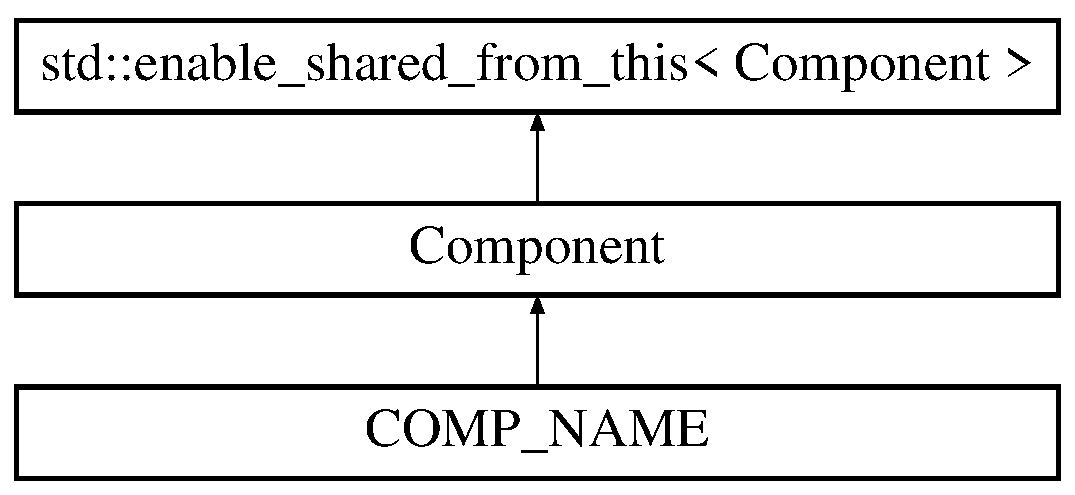
\includegraphics[height=3.000000cm]{classCOMP__NAME}
\end{center}
\end{figure}
\subsection*{Public Member Functions}
\begin{DoxyCompactItemize}
\item 
\mbox{\Hypertarget{classCOMP__NAME_a5e5144cab5540c8102c3c03a0ee0a768}\label{classCOMP__NAME_a5e5144cab5540c8102c3c03a0ee0a768}} 
{\bfseries C\+O\+M\+P\+\_\+\+N\+A\+ME} (std\+::shared\+\_\+ptr$<$ \hyperlink{classSpaCommunicator}{Spa\+Communicator} $>$ com=nullptr)
\item 
\mbox{\Hypertarget{classCOMP__NAME_a8c1d575e72e948f84891244ca3bee646}\label{classCOMP__NAME_a8c1d575e72e948f84891244ca3bee646}} 
void {\bfseries handle\+Spa\+Data} (\hyperlink{structSpaMessage}{Spa\+Message} $\ast$message)
\item 
\mbox{\Hypertarget{classCOMP__NAME_ac981fe25a24ee01c160d08f0a970fab1}\label{classCOMP__NAME_ac981fe25a24ee01c160d08f0a970fab1}} 
void {\bfseries send\+Data} (\hyperlink{structLogicalAddress}{Logical\+Address} destination)
\item 
\mbox{\Hypertarget{classCOMP__NAME_abfae2e6e6f24cee4c16800385a103ca8}\label{classCOMP__NAME_abfae2e6e6f24cee4c16800385a103ca8}} 
void {\bfseries init} ()
\end{DoxyCompactItemize}
\subsection*{Additional Inherited Members}


The documentation for this class was generated from the following file\+:\begin{DoxyCompactItemize}
\item 
drivers/\+Temp\+Sensor/Temp\+Sensor.\+cpp\end{DoxyCompactItemize}

\hypertarget{classComponent}{}\section{Component Class Reference}
\label{classComponent}\index{Component@{Component}}


{\ttfamily \#include $<$component.\+hpp$>$}

Inheritance diagram for Component\+:\begin{figure}[H]
\begin{center}
\leavevmode
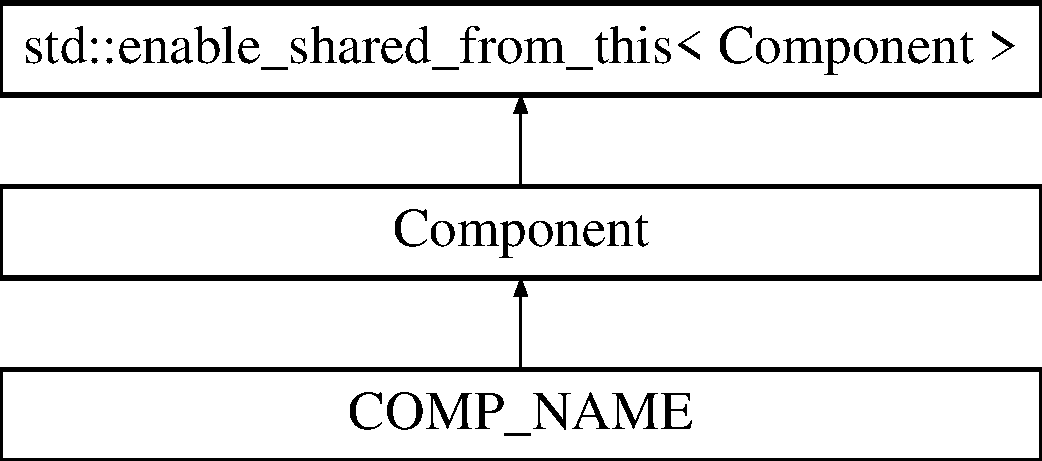
\includegraphics[height=3.000000cm]{classComponent}
\end{center}
\end{figure}
\subsection*{Public Member Functions}
\begin{DoxyCompactItemize}
\item 
\hyperlink{classComponent_a83f43d60a90000cfd63aca351ba648c4}{Component} (std\+::shared\+\_\+ptr$<$ \hyperlink{classSpaCommunicator}{Spa\+Communicator} $>$ \hyperlink{classComponent_ab124decba1547f96b7df055e3b7e902e}{communicator}=nullptr, \hyperlink{structLogicalAddress}{Logical\+Address} \hyperlink{classComponent_aa60ef4220c2630dde612e2f0164b3676}{address}=\hyperlink{structLogicalAddress}{Logical\+Address}(0, 0), \hyperlink{structLogicalAddress}{Logical\+Address} \hyperlink{classComponent_a8147bae546da489c3ffa5a1a634739a0}{subnet\+Manager\+Address}=\hyperlink{structLogicalAddress}{Logical\+Address}(0, 0))
\item 
virtual \hyperlink{classComponent_a2e9aa4348314d981f05f67397ad2f872}{$\sim$\+Component} ()
\item 
void \hyperlink{classComponent_a22b96395923537ce1a56692fdd971749}{publish} ()
\item 
virtual void \hyperlink{classComponent_a0f71f7a7ff6c0e7cd28692b6890a0058}{handle\+Spa\+Data} (\hyperlink{structSpaMessage}{Spa\+Message} $\ast$)=0
\item 
virtual void \hyperlink{classComponent_a9e6d270061f52a3b42e9d2b0fd8f65c2}{pre\+Init} ()
\item 
virtual void \hyperlink{classComponent_a2bbe062eb418a541fd0cfbcfdf3f55b0}{listen} ()
\item 
virtual void \hyperlink{classComponent_a56baf8afdea3366554b3c7b13fd6e3f7}{init} ()=0
\item 
void \hyperlink{classComponent_a4fe6afd53663b5c1d3b60977024bc86a}{send\+Msg} (\hyperlink{structSpaMessage}{Spa\+Message} $\ast$message, ssize\+\_\+t len)
\item 
void \hyperlink{classComponent_a3142ee952db05b1352f539d446f63934}{receive\+Message} (\hyperlink{structSpaMessage}{Spa\+Message} $\ast$)
\item 
void \hyperlink{classComponent_af387d0bc27df38fc6c797d6d3329697a}{handle\+Subscription\+Reply} (\hyperlink{structSpaMessage}{Spa\+Message} $\ast$)
\item 
void \hyperlink{classComponent_aaa5c27b493d39887885adb3dd21e2224}{register\+Subscription\+Request} (\hyperlink{structSpaMessage}{Spa\+Message} $\ast$)
\item 
void \hyperlink{classComponent_a9f81ad79e0243e6e52ae04b26e6657ab}{receive\+Buffer} (\hyperlink{structcubiumClientSocket__t}{cubium\+Client\+Socket\+\_\+t} $\ast$)
\item 
void \hyperlink{classComponent_a55c74b1c2dcde114cb329ae43a4cd04a}{subscribe} (\hyperlink{structLogicalAddress}{Logical\+Address} producer)
\item 
void \hyperlink{classComponent_abae1852e26a7bee748898ea8ef6f4fb9}{subscribe} (\hyperlink{structLogicalAddress}{Logical\+Address} producer, uint8\+\_\+t priority, uint32\+\_\+t lease\+Period, uint16\+\_\+t delivery\+Rate\+Divisor)
\item 
virtual void \hyperlink{classComponent_a492a20dc97b9563d80443dda2f1057ec}{send\+Data} (\hyperlink{structLogicalAddress}{Logical\+Address})=0
\item 
void \hyperlink{classComponent_afc9525526fdc44c64873abf80357c3be}{send\+Payload} (std\+::string payload, \hyperlink{structLogicalAddress}{Logical\+Address} destination)
\item 
{\footnotesize template$<$typename T $>$ }\\void \hyperlink{classComponent_af7ee2839809098ffd50029375aa3e5a7}{send\+Payload} (T payload, \hyperlink{structLogicalAddress}{Logical\+Address} destination)
\item 
bool \hyperlink{classComponent_a54c0c489eec4e4f6b23655a734fc00d4}{add\+Subscriber} (\hyperlink{structLogicalAddress}{Logical\+Address}, uint16\+\_\+t)
\end{DoxyCompactItemize}
\subsection*{Public Attributes}
\begin{DoxyCompactItemize}
\item 
std\+::shared\+\_\+ptr$<$ \hyperlink{classSpaCommunicator}{Spa\+Communicator} $>$ \hyperlink{classComponent_ab124decba1547f96b7df055e3b7e902e}{communicator}
\item 
std\+::vector$<$ \hyperlink{structSubscriber}{Subscriber} $>$ \hyperlink{classComponent_a4b1fc3511ba706058d5e575e5b4b55f7}{subscribers}
\item 
std\+::mutex \hyperlink{classComponent_ad289c568dee48290561f885d69f09d94}{m\+\_\+subscribers}
\end{DoxyCompactItemize}
\subsection*{Protected Attributes}
\begin{DoxyCompactItemize}
\item 
\hyperlink{structLogicalAddress}{Logical\+Address} \hyperlink{classComponent_aa60ef4220c2630dde612e2f0164b3676}{address}
\item 
\hyperlink{structLogicalAddress}{Logical\+Address} \hyperlink{classComponent_a8147bae546da489c3ffa5a1a634739a0}{subnet\+Manager\+Address}
\item 
uint8\+\_\+t \hyperlink{classComponent_a5dff98c7893ff79b6ff35cdc26f65240}{publish\+Iter}
\item 
uint16\+\_\+t \hyperlink{classComponent_a6d22415eb4e07f9cc5a5c917972bf0dd}{dialog\+Id}
\item 
\hyperlink{structSpaCourier}{Spa\+Courier} $\ast$ \hyperlink{classComponent_ab8aa5882c1e2c8139e3ec9d9d27ff174}{last\+Courier}
\end{DoxyCompactItemize}


\subsection{Constructor \& Destructor Documentation}
\mbox{\Hypertarget{classComponent_a83f43d60a90000cfd63aca351ba648c4}\label{classComponent_a83f43d60a90000cfd63aca351ba648c4}} 
\index{Component@{Component}!Component@{Component}}
\index{Component@{Component}!Component@{Component}}
\subsubsection{\texorpdfstring{Component()}{Component()}}
{\footnotesize\ttfamily Component\+::\+Component (\begin{DoxyParamCaption}\item[{std\+::shared\+\_\+ptr$<$ \hyperlink{classSpaCommunicator}{Spa\+Communicator} $>$}]{communicator = {\ttfamily nullptr},  }\item[{\hyperlink{structLogicalAddress}{Logical\+Address}}]{address = {\ttfamily \hyperlink{structLogicalAddress}{Logical\+Address}(0,~0)},  }\item[{\hyperlink{structLogicalAddress}{Logical\+Address}}]{subnet\+Manager\+Address = {\ttfamily \hyperlink{structLogicalAddress}{Logical\+Address}(0,~0)} }\end{DoxyParamCaption})\hspace{0.3cm}{\ttfamily [inline]}}

\mbox{\Hypertarget{classComponent_a2e9aa4348314d981f05f67397ad2f872}\label{classComponent_a2e9aa4348314d981f05f67397ad2f872}} 
\index{Component@{Component}!````~Component@{$\sim$\+Component}}
\index{````~Component@{$\sim$\+Component}!Component@{Component}}
\subsubsection{\texorpdfstring{$\sim$\+Component()}{~Component()}}
{\footnotesize\ttfamily virtual Component\+::$\sim$\+Component (\begin{DoxyParamCaption}{ }\end{DoxyParamCaption})\hspace{0.3cm}{\ttfamily [inline]}, {\ttfamily [virtual]}}



\subsection{Member Function Documentation}
\mbox{\Hypertarget{classComponent_a54c0c489eec4e4f6b23655a734fc00d4}\label{classComponent_a54c0c489eec4e4f6b23655a734fc00d4}} 
\index{Component@{Component}!add\+Subscriber@{add\+Subscriber}}
\index{add\+Subscriber@{add\+Subscriber}!Component@{Component}}
\subsubsection{\texorpdfstring{add\+Subscriber()}{addSubscriber()}}
{\footnotesize\ttfamily bool Component\+::add\+Subscriber (\begin{DoxyParamCaption}\item[{\hyperlink{structLogicalAddress}{Logical\+Address}}]{la,  }\item[{uint16\+\_\+t}]{d }\end{DoxyParamCaption})}

\mbox{\Hypertarget{classComponent_a0f71f7a7ff6c0e7cd28692b6890a0058}\label{classComponent_a0f71f7a7ff6c0e7cd28692b6890a0058}} 
\index{Component@{Component}!handle\+Spa\+Data@{handle\+Spa\+Data}}
\index{handle\+Spa\+Data@{handle\+Spa\+Data}!Component@{Component}}
\subsubsection{\texorpdfstring{handle\+Spa\+Data()}{handleSpaData()}}
{\footnotesize\ttfamily virtual void Component\+::handle\+Spa\+Data (\begin{DoxyParamCaption}\item[{\hyperlink{structSpaMessage}{Spa\+Message} $\ast$}]{ }\end{DoxyParamCaption})\hspace{0.3cm}{\ttfamily [pure virtual]}}



Implemented in \hyperlink{classCOMP__NAME_a8c1d575e72e948f84891244ca3bee646}{C\+O\+M\+P\+\_\+\+N\+A\+ME}.

\mbox{\Hypertarget{classComponent_af387d0bc27df38fc6c797d6d3329697a}\label{classComponent_af387d0bc27df38fc6c797d6d3329697a}} 
\index{Component@{Component}!handle\+Subscription\+Reply@{handle\+Subscription\+Reply}}
\index{handle\+Subscription\+Reply@{handle\+Subscription\+Reply}!Component@{Component}}
\subsubsection{\texorpdfstring{handle\+Subscription\+Reply()}{handleSubscriptionReply()}}
{\footnotesize\ttfamily void Component\+::handle\+Subscription\+Reply (\begin{DoxyParamCaption}\item[{\hyperlink{structSpaMessage}{Spa\+Message} $\ast$}]{message }\end{DoxyParamCaption})}

\mbox{\Hypertarget{classComponent_a56baf8afdea3366554b3c7b13fd6e3f7}\label{classComponent_a56baf8afdea3366554b3c7b13fd6e3f7}} 
\index{Component@{Component}!init@{init}}
\index{init@{init}!Component@{Component}}
\subsubsection{\texorpdfstring{init()}{init()}}
{\footnotesize\ttfamily virtual void Component\+::init (\begin{DoxyParamCaption}{ }\end{DoxyParamCaption})\hspace{0.3cm}{\ttfamily [pure virtual]}}



Implemented in \hyperlink{classCOMP__NAME_abfae2e6e6f24cee4c16800385a103ca8}{C\+O\+M\+P\+\_\+\+N\+A\+ME}.

\mbox{\Hypertarget{classComponent_a2bbe062eb418a541fd0cfbcfdf3f55b0}\label{classComponent_a2bbe062eb418a541fd0cfbcfdf3f55b0}} 
\index{Component@{Component}!listen@{listen}}
\index{listen@{listen}!Component@{Component}}
\subsubsection{\texorpdfstring{listen()}{listen()}}
{\footnotesize\ttfamily virtual void Component\+::listen (\begin{DoxyParamCaption}{ }\end{DoxyParamCaption})\hspace{0.3cm}{\ttfamily [inline]}, {\ttfamily [virtual]}}

\mbox{\Hypertarget{classComponent_a9e6d270061f52a3b42e9d2b0fd8f65c2}\label{classComponent_a9e6d270061f52a3b42e9d2b0fd8f65c2}} 
\index{Component@{Component}!pre\+Init@{pre\+Init}}
\index{pre\+Init@{pre\+Init}!Component@{Component}}
\subsubsection{\texorpdfstring{pre\+Init()}{preInit()}}
{\footnotesize\ttfamily virtual void Component\+::pre\+Init (\begin{DoxyParamCaption}{ }\end{DoxyParamCaption})\hspace{0.3cm}{\ttfamily [inline]}, {\ttfamily [virtual]}}

\mbox{\Hypertarget{classComponent_a22b96395923537ce1a56692fdd971749}\label{classComponent_a22b96395923537ce1a56692fdd971749}} 
\index{Component@{Component}!publish@{publish}}
\index{publish@{publish}!Component@{Component}}
\subsubsection{\texorpdfstring{publish()}{publish()}}
{\footnotesize\ttfamily void Component\+::publish (\begin{DoxyParamCaption}{ }\end{DoxyParamCaption})}

\mbox{\Hypertarget{classComponent_a9f81ad79e0243e6e52ae04b26e6657ab}\label{classComponent_a9f81ad79e0243e6e52ae04b26e6657ab}} 
\index{Component@{Component}!receive\+Buffer@{receive\+Buffer}}
\index{receive\+Buffer@{receive\+Buffer}!Component@{Component}}
\subsubsection{\texorpdfstring{receive\+Buffer()}{receiveBuffer()}}
{\footnotesize\ttfamily void Component\+::receive\+Buffer (\begin{DoxyParamCaption}\item[{\hyperlink{structcubiumClientSocket__t}{cubium\+Client\+Socket\+\_\+t} $\ast$}]{sock }\end{DoxyParamCaption})}

\mbox{\Hypertarget{classComponent_a3142ee952db05b1352f539d446f63934}\label{classComponent_a3142ee952db05b1352f539d446f63934}} 
\index{Component@{Component}!receive\+Message@{receive\+Message}}
\index{receive\+Message@{receive\+Message}!Component@{Component}}
\subsubsection{\texorpdfstring{receive\+Message()}{receiveMessage()}}
{\footnotesize\ttfamily void Component\+::receive\+Message (\begin{DoxyParamCaption}\item[{\hyperlink{structSpaMessage}{Spa\+Message} $\ast$}]{message }\end{DoxyParamCaption})}

\mbox{\Hypertarget{classComponent_aaa5c27b493d39887885adb3dd21e2224}\label{classComponent_aaa5c27b493d39887885adb3dd21e2224}} 
\index{Component@{Component}!register\+Subscription\+Request@{register\+Subscription\+Request}}
\index{register\+Subscription\+Request@{register\+Subscription\+Request}!Component@{Component}}
\subsubsection{\texorpdfstring{register\+Subscription\+Request()}{registerSubscriptionRequest()}}
{\footnotesize\ttfamily void Component\+::register\+Subscription\+Request (\begin{DoxyParamCaption}\item[{\hyperlink{structSpaMessage}{Spa\+Message} $\ast$}]{message }\end{DoxyParamCaption})}

\mbox{\Hypertarget{classComponent_a492a20dc97b9563d80443dda2f1057ec}\label{classComponent_a492a20dc97b9563d80443dda2f1057ec}} 
\index{Component@{Component}!send\+Data@{send\+Data}}
\index{send\+Data@{send\+Data}!Component@{Component}}
\subsubsection{\texorpdfstring{send\+Data()}{sendData()}}
{\footnotesize\ttfamily virtual void Component\+::send\+Data (\begin{DoxyParamCaption}\item[{\hyperlink{structLogicalAddress}{Logical\+Address}}]{ }\end{DoxyParamCaption})\hspace{0.3cm}{\ttfamily [pure virtual]}}



Implemented in \hyperlink{classCOMP__NAME_ac981fe25a24ee01c160d08f0a970fab1}{C\+O\+M\+P\+\_\+\+N\+A\+ME}.

\mbox{\Hypertarget{classComponent_a4fe6afd53663b5c1d3b60977024bc86a}\label{classComponent_a4fe6afd53663b5c1d3b60977024bc86a}} 
\index{Component@{Component}!send\+Msg@{send\+Msg}}
\index{send\+Msg@{send\+Msg}!Component@{Component}}
\subsubsection{\texorpdfstring{send\+Msg()}{sendMsg()}}
{\footnotesize\ttfamily void Component\+::send\+Msg (\begin{DoxyParamCaption}\item[{\hyperlink{structSpaMessage}{Spa\+Message} $\ast$}]{message,  }\item[{ssize\+\_\+t}]{len }\end{DoxyParamCaption})\hspace{0.3cm}{\ttfamily [inline]}}

\mbox{\Hypertarget{classComponent_afc9525526fdc44c64873abf80357c3be}\label{classComponent_afc9525526fdc44c64873abf80357c3be}} 
\index{Component@{Component}!send\+Payload@{send\+Payload}}
\index{send\+Payload@{send\+Payload}!Component@{Component}}
\subsubsection{\texorpdfstring{send\+Payload()}{sendPayload()}\hspace{0.1cm}{\footnotesize\ttfamily [1/2]}}
{\footnotesize\ttfamily void Component\+::send\+Payload (\begin{DoxyParamCaption}\item[{std\+::string}]{payload,  }\item[{\hyperlink{structLogicalAddress}{Logical\+Address}}]{destination }\end{DoxyParamCaption})\hspace{0.3cm}{\ttfamily [inline]}}

\mbox{\Hypertarget{classComponent_af7ee2839809098ffd50029375aa3e5a7}\label{classComponent_af7ee2839809098ffd50029375aa3e5a7}} 
\index{Component@{Component}!send\+Payload@{send\+Payload}}
\index{send\+Payload@{send\+Payload}!Component@{Component}}
\subsubsection{\texorpdfstring{send\+Payload()}{sendPayload()}\hspace{0.1cm}{\footnotesize\ttfamily [2/2]}}
{\footnotesize\ttfamily template$<$typename T $>$ \\
void Component\+::send\+Payload (\begin{DoxyParamCaption}\item[{T}]{payload,  }\item[{\hyperlink{structLogicalAddress}{Logical\+Address}}]{destination }\end{DoxyParamCaption})\hspace{0.3cm}{\ttfamily [inline]}}

\mbox{\Hypertarget{classComponent_a55c74b1c2dcde114cb329ae43a4cd04a}\label{classComponent_a55c74b1c2dcde114cb329ae43a4cd04a}} 
\index{Component@{Component}!subscribe@{subscribe}}
\index{subscribe@{subscribe}!Component@{Component}}
\subsubsection{\texorpdfstring{subscribe()}{subscribe()}\hspace{0.1cm}{\footnotesize\ttfamily [1/2]}}
{\footnotesize\ttfamily void Component\+::subscribe (\begin{DoxyParamCaption}\item[{\hyperlink{structLogicalAddress}{Logical\+Address}}]{producer }\end{DoxyParamCaption})\hspace{0.3cm}{\ttfamily [inline]}}

\mbox{\Hypertarget{classComponent_abae1852e26a7bee748898ea8ef6f4fb9}\label{classComponent_abae1852e26a7bee748898ea8ef6f4fb9}} 
\index{Component@{Component}!subscribe@{subscribe}}
\index{subscribe@{subscribe}!Component@{Component}}
\subsubsection{\texorpdfstring{subscribe()}{subscribe()}\hspace{0.1cm}{\footnotesize\ttfamily [2/2]}}
{\footnotesize\ttfamily void Component\+::subscribe (\begin{DoxyParamCaption}\item[{\hyperlink{structLogicalAddress}{Logical\+Address}}]{producer,  }\item[{uint8\+\_\+t}]{priority,  }\item[{uint32\+\_\+t}]{lease\+Period,  }\item[{uint16\+\_\+t}]{delivery\+Rate\+Divisor }\end{DoxyParamCaption})}



\subsection{Member Data Documentation}
\mbox{\Hypertarget{classComponent_aa60ef4220c2630dde612e2f0164b3676}\label{classComponent_aa60ef4220c2630dde612e2f0164b3676}} 
\index{Component@{Component}!address@{address}}
\index{address@{address}!Component@{Component}}
\subsubsection{\texorpdfstring{address}{address}}
{\footnotesize\ttfamily \hyperlink{structLogicalAddress}{Logical\+Address} Component\+::address\hspace{0.3cm}{\ttfamily [protected]}}

\mbox{\Hypertarget{classComponent_ab124decba1547f96b7df055e3b7e902e}\label{classComponent_ab124decba1547f96b7df055e3b7e902e}} 
\index{Component@{Component}!communicator@{communicator}}
\index{communicator@{communicator}!Component@{Component}}
\subsubsection{\texorpdfstring{communicator}{communicator}}
{\footnotesize\ttfamily std\+::shared\+\_\+ptr$<$\hyperlink{classSpaCommunicator}{Spa\+Communicator}$>$ Component\+::communicator}

\mbox{\Hypertarget{classComponent_a6d22415eb4e07f9cc5a5c917972bf0dd}\label{classComponent_a6d22415eb4e07f9cc5a5c917972bf0dd}} 
\index{Component@{Component}!dialog\+Id@{dialog\+Id}}
\index{dialog\+Id@{dialog\+Id}!Component@{Component}}
\subsubsection{\texorpdfstring{dialog\+Id}{dialogId}}
{\footnotesize\ttfamily uint16\+\_\+t Component\+::dialog\+Id\hspace{0.3cm}{\ttfamily [protected]}}

\mbox{\Hypertarget{classComponent_ab8aa5882c1e2c8139e3ec9d9d27ff174}\label{classComponent_ab8aa5882c1e2c8139e3ec9d9d27ff174}} 
\index{Component@{Component}!last\+Courier@{last\+Courier}}
\index{last\+Courier@{last\+Courier}!Component@{Component}}
\subsubsection{\texorpdfstring{last\+Courier}{lastCourier}}
{\footnotesize\ttfamily \hyperlink{structSpaCourier}{Spa\+Courier}$\ast$ Component\+::last\+Courier\hspace{0.3cm}{\ttfamily [protected]}}

\mbox{\Hypertarget{classComponent_ad289c568dee48290561f885d69f09d94}\label{classComponent_ad289c568dee48290561f885d69f09d94}} 
\index{Component@{Component}!m\+\_\+subscribers@{m\+\_\+subscribers}}
\index{m\+\_\+subscribers@{m\+\_\+subscribers}!Component@{Component}}
\subsubsection{\texorpdfstring{m\+\_\+subscribers}{m\_subscribers}}
{\footnotesize\ttfamily std\+::mutex Component\+::m\+\_\+subscribers}

\mbox{\Hypertarget{classComponent_a5dff98c7893ff79b6ff35cdc26f65240}\label{classComponent_a5dff98c7893ff79b6ff35cdc26f65240}} 
\index{Component@{Component}!publish\+Iter@{publish\+Iter}}
\index{publish\+Iter@{publish\+Iter}!Component@{Component}}
\subsubsection{\texorpdfstring{publish\+Iter}{publishIter}}
{\footnotesize\ttfamily uint8\+\_\+t Component\+::publish\+Iter\hspace{0.3cm}{\ttfamily [protected]}}

\mbox{\Hypertarget{classComponent_a8147bae546da489c3ffa5a1a634739a0}\label{classComponent_a8147bae546da489c3ffa5a1a634739a0}} 
\index{Component@{Component}!subnet\+Manager\+Address@{subnet\+Manager\+Address}}
\index{subnet\+Manager\+Address@{subnet\+Manager\+Address}!Component@{Component}}
\subsubsection{\texorpdfstring{subnet\+Manager\+Address}{subnetManagerAddress}}
{\footnotesize\ttfamily \hyperlink{structLogicalAddress}{Logical\+Address} Component\+::subnet\+Manager\+Address\hspace{0.3cm}{\ttfamily [protected]}}

\mbox{\Hypertarget{classComponent_a4b1fc3511ba706058d5e575e5b4b55f7}\label{classComponent_a4b1fc3511ba706058d5e575e5b4b55f7}} 
\index{Component@{Component}!subscribers@{subscribers}}
\index{subscribers@{subscribers}!Component@{Component}}
\subsubsection{\texorpdfstring{subscribers}{subscribers}}
{\footnotesize\ttfamily std\+::vector$<$\hyperlink{structSubscriber}{Subscriber}$>$ Component\+::subscribers}



The documentation for this class was generated from the following files\+:\begin{DoxyCompactItemize}
\item 
lib/\hyperlink{component_8hpp}{component.\+hpp}\item 
lib/\hyperlink{component_8cpp}{component.\+cpp}\end{DoxyCompactItemize}

\hypertarget{structComponentInfo}{}\section{Component\+Info Struct Reference}
\label{structComponentInfo}\index{Component\+Info@{Component\+Info}}


{\ttfamily \#include $<$component\+\_\+list.\+hpp$>$}

\subsection*{Public Member Functions}
\begin{DoxyCompactItemize}
\item 
\hyperlink{structComponentInfo_aa02e1576e688c7883e97e242a804cff4}{Component\+Info} (\hyperlink{structLogicalAddress}{Logical\+Address} la, bool h)
\end{DoxyCompactItemize}
\subsection*{Public Attributes}
\begin{DoxyCompactItemize}
\item 
\hyperlink{structLogicalAddress}{Logical\+Address} \hyperlink{structComponentInfo_a0ebb1e5717838ca670048317eeda0bed}{address}
\item 
bool \hyperlink{structComponentInfo_af3eec118fc95855cf27a9825f04a659c}{healthy} = true
\end{DoxyCompactItemize}


\subsection{Constructor \& Destructor Documentation}
\mbox{\Hypertarget{structComponentInfo_aa02e1576e688c7883e97e242a804cff4}\label{structComponentInfo_aa02e1576e688c7883e97e242a804cff4}} 
\index{Component\+Info@{Component\+Info}!Component\+Info@{Component\+Info}}
\index{Component\+Info@{Component\+Info}!Component\+Info@{Component\+Info}}
\subsubsection{\texorpdfstring{Component\+Info()}{ComponentInfo()}}
{\footnotesize\ttfamily Component\+Info\+::\+Component\+Info (\begin{DoxyParamCaption}\item[{\hyperlink{structLogicalAddress}{Logical\+Address}}]{la,  }\item[{bool}]{h }\end{DoxyParamCaption})\hspace{0.3cm}{\ttfamily [inline]}}



\subsection{Member Data Documentation}
\mbox{\Hypertarget{structComponentInfo_a0ebb1e5717838ca670048317eeda0bed}\label{structComponentInfo_a0ebb1e5717838ca670048317eeda0bed}} 
\index{Component\+Info@{Component\+Info}!address@{address}}
\index{address@{address}!Component\+Info@{Component\+Info}}
\subsubsection{\texorpdfstring{address}{address}}
{\footnotesize\ttfamily \hyperlink{structLogicalAddress}{Logical\+Address} Component\+Info\+::address}

\mbox{\Hypertarget{structComponentInfo_af3eec118fc95855cf27a9825f04a659c}\label{structComponentInfo_af3eec118fc95855cf27a9825f04a659c}} 
\index{Component\+Info@{Component\+Info}!healthy@{healthy}}
\index{healthy@{healthy}!Component\+Info@{Component\+Info}}
\subsubsection{\texorpdfstring{healthy}{healthy}}
{\footnotesize\ttfamily bool Component\+Info\+::healthy = true}



The documentation for this struct was generated from the following file\+:\begin{DoxyCompactItemize}
\item 
lib/\hyperlink{component__list_8hpp}{component\+\_\+list.\+hpp}\end{DoxyCompactItemize}

\hypertarget{classComponentList}{}\section{Component\+List Class Reference}
\label{classComponentList}\index{Component\+List@{Component\+List}}


{\ttfamily \#include $<$component\+\_\+list.\+hpp$>$}

\subsection*{Public Member Functions}
\begin{DoxyCompactItemize}
\item 
\hyperlink{classComponentList_a15ab6b476094b0ee17090086e6cec168}{Component\+List} ()
\item 
\hyperlink{classComponentList_ab260978fcc65754d836c6a3cb8b42341}{Component\+List} (\hyperlink{structLogicalAddress}{Logical\+Address} l)
\item 
void \hyperlink{classComponentList_a16746faf0795286b07d34315506a0940}{add} (\hyperlink{structLogicalAddress}{Logical\+Address} la)
\item 
\hyperlink{structLogicalAddress}{Logical\+Address} \hyperlink{classComponentList_a19d60f3644b19fa267ea669e2e47d409}{get\+Address} (int i)
\end{DoxyCompactItemize}
\subsection*{Protected Attributes}
\begin{DoxyCompactItemize}
\item 
std\+::vector$<$ \hyperlink{structComponentInfo}{Component\+Info} $>$ \hyperlink{classComponentList_abab41b240f17f716229e5abd5279dd9b}{list}
\end{DoxyCompactItemize}


\subsection{Constructor \& Destructor Documentation}
\mbox{\Hypertarget{classComponentList_a15ab6b476094b0ee17090086e6cec168}\label{classComponentList_a15ab6b476094b0ee17090086e6cec168}} 
\index{Component\+List@{Component\+List}!Component\+List@{Component\+List}}
\index{Component\+List@{Component\+List}!Component\+List@{Component\+List}}
\subsubsection{\texorpdfstring{Component\+List()}{ComponentList()}\hspace{0.1cm}{\footnotesize\ttfamily [1/2]}}
{\footnotesize\ttfamily Component\+List\+::\+Component\+List (\begin{DoxyParamCaption}{ }\end{DoxyParamCaption})\hspace{0.3cm}{\ttfamily [inline]}}

\mbox{\Hypertarget{classComponentList_ab260978fcc65754d836c6a3cb8b42341}\label{classComponentList_ab260978fcc65754d836c6a3cb8b42341}} 
\index{Component\+List@{Component\+List}!Component\+List@{Component\+List}}
\index{Component\+List@{Component\+List}!Component\+List@{Component\+List}}
\subsubsection{\texorpdfstring{Component\+List()}{ComponentList()}\hspace{0.1cm}{\footnotesize\ttfamily [2/2]}}
{\footnotesize\ttfamily Component\+List\+::\+Component\+List (\begin{DoxyParamCaption}\item[{\hyperlink{structLogicalAddress}{Logical\+Address}}]{l }\end{DoxyParamCaption})\hspace{0.3cm}{\ttfamily [inline]}}



\subsection{Member Function Documentation}
\mbox{\Hypertarget{classComponentList_a16746faf0795286b07d34315506a0940}\label{classComponentList_a16746faf0795286b07d34315506a0940}} 
\index{Component\+List@{Component\+List}!add@{add}}
\index{add@{add}!Component\+List@{Component\+List}}
\subsubsection{\texorpdfstring{add()}{add()}}
{\footnotesize\ttfamily void Component\+List\+::add (\begin{DoxyParamCaption}\item[{\hyperlink{structLogicalAddress}{Logical\+Address}}]{la }\end{DoxyParamCaption})\hspace{0.3cm}{\ttfamily [inline]}}

\mbox{\Hypertarget{classComponentList_a19d60f3644b19fa267ea669e2e47d409}\label{classComponentList_a19d60f3644b19fa267ea669e2e47d409}} 
\index{Component\+List@{Component\+List}!get\+Address@{get\+Address}}
\index{get\+Address@{get\+Address}!Component\+List@{Component\+List}}
\subsubsection{\texorpdfstring{get\+Address()}{getAddress()}}
{\footnotesize\ttfamily \hyperlink{structLogicalAddress}{Logical\+Address} Component\+List\+::get\+Address (\begin{DoxyParamCaption}\item[{int}]{i }\end{DoxyParamCaption})\hspace{0.3cm}{\ttfamily [inline]}}



\subsection{Member Data Documentation}
\mbox{\Hypertarget{classComponentList_abab41b240f17f716229e5abd5279dd9b}\label{classComponentList_abab41b240f17f716229e5abd5279dd9b}} 
\index{Component\+List@{Component\+List}!list@{list}}
\index{list@{list}!Component\+List@{Component\+List}}
\subsubsection{\texorpdfstring{list}{list}}
{\footnotesize\ttfamily std\+::vector$<$\hyperlink{structComponentInfo}{Component\+Info}$>$ Component\+List\+::list\hspace{0.3cm}{\ttfamily [protected]}}



The documentation for this class was generated from the following file\+:\begin{DoxyCompactItemize}
\item 
lib/\hyperlink{component__list_8hpp}{component\+\_\+list.\+hpp}\end{DoxyCompactItemize}

\hypertarget{structcubiumClientSocket__t}{}\section{cubium\+Client\+Socket\+\_\+t Struct Reference}
\label{structcubiumClientSocket__t}\index{cubium\+Client\+Socket\+\_\+t@{cubium\+Client\+Socket\+\_\+t}}


{\ttfamily \#include $<$client\+Socket.\+hpp$>$}

\subsection*{Public Attributes}
\begin{DoxyCompactItemize}
\item 
uint32\+\_\+t \hyperlink{structcubiumClientSocket__t_abaa0344892988ffb56dea7f82b88cbc3}{sock}
\item 
uint32\+\_\+t \hyperlink{structcubiumClientSocket__t_af0fb9d2f6a29407f9efb5cbc9da1f314}{n\+Bytes\+Recv}
\item 
uint32\+\_\+t \hyperlink{structcubiumClientSocket__t_a1328962fd1aceb332accc664f006f35c}{length}
\item 
struct sockaddr\+\_\+in \hyperlink{structcubiumClientSocket__t_ad89460d48cb94e5cda49ed0481e927f1}{server}
\item 
struct sockaddr\+\_\+in \hyperlink{structcubiumClientSocket__t_adbcedcdc98e808414c6b08b41d3a3450}{from}
\item 
struct hostent $\ast$ \hyperlink{structcubiumClientSocket__t_a976b1153569e15360062775633f759fa}{hp}
\item 
char \hyperlink{structcubiumClientSocket__t_af4af5909ff1caa85848438449d1edc91}{buf} \mbox{[}256\mbox{]}
\item 
bool \hyperlink{structcubiumClientSocket__t_aa796f9502f1416372e62080b9e1a7446}{is\+Buf} = false
\end{DoxyCompactItemize}


\subsection{Member Data Documentation}
\mbox{\Hypertarget{structcubiumClientSocket__t_af4af5909ff1caa85848438449d1edc91}\label{structcubiumClientSocket__t_af4af5909ff1caa85848438449d1edc91}} 
\index{cubium\+Client\+Socket\+\_\+t@{cubium\+Client\+Socket\+\_\+t}!buf@{buf}}
\index{buf@{buf}!cubium\+Client\+Socket\+\_\+t@{cubium\+Client\+Socket\+\_\+t}}
\subsubsection{\texorpdfstring{buf}{buf}}
{\footnotesize\ttfamily char cubium\+Client\+Socket\+\_\+t\+::buf\mbox{[}256\mbox{]}}

\mbox{\Hypertarget{structcubiumClientSocket__t_adbcedcdc98e808414c6b08b41d3a3450}\label{structcubiumClientSocket__t_adbcedcdc98e808414c6b08b41d3a3450}} 
\index{cubium\+Client\+Socket\+\_\+t@{cubium\+Client\+Socket\+\_\+t}!from@{from}}
\index{from@{from}!cubium\+Client\+Socket\+\_\+t@{cubium\+Client\+Socket\+\_\+t}}
\subsubsection{\texorpdfstring{from}{from}}
{\footnotesize\ttfamily struct sockaddr\+\_\+in cubium\+Client\+Socket\+\_\+t\+::from}

\mbox{\Hypertarget{structcubiumClientSocket__t_a976b1153569e15360062775633f759fa}\label{structcubiumClientSocket__t_a976b1153569e15360062775633f759fa}} 
\index{cubium\+Client\+Socket\+\_\+t@{cubium\+Client\+Socket\+\_\+t}!hp@{hp}}
\index{hp@{hp}!cubium\+Client\+Socket\+\_\+t@{cubium\+Client\+Socket\+\_\+t}}
\subsubsection{\texorpdfstring{hp}{hp}}
{\footnotesize\ttfamily struct hostent$\ast$ cubium\+Client\+Socket\+\_\+t\+::hp}

\mbox{\Hypertarget{structcubiumClientSocket__t_aa796f9502f1416372e62080b9e1a7446}\label{structcubiumClientSocket__t_aa796f9502f1416372e62080b9e1a7446}} 
\index{cubium\+Client\+Socket\+\_\+t@{cubium\+Client\+Socket\+\_\+t}!is\+Buf@{is\+Buf}}
\index{is\+Buf@{is\+Buf}!cubium\+Client\+Socket\+\_\+t@{cubium\+Client\+Socket\+\_\+t}}
\subsubsection{\texorpdfstring{is\+Buf}{isBuf}}
{\footnotesize\ttfamily bool cubium\+Client\+Socket\+\_\+t\+::is\+Buf = false}

\mbox{\Hypertarget{structcubiumClientSocket__t_a1328962fd1aceb332accc664f006f35c}\label{structcubiumClientSocket__t_a1328962fd1aceb332accc664f006f35c}} 
\index{cubium\+Client\+Socket\+\_\+t@{cubium\+Client\+Socket\+\_\+t}!length@{length}}
\index{length@{length}!cubium\+Client\+Socket\+\_\+t@{cubium\+Client\+Socket\+\_\+t}}
\subsubsection{\texorpdfstring{length}{length}}
{\footnotesize\ttfamily uint32\+\_\+t cubium\+Client\+Socket\+\_\+t\+::length}

\mbox{\Hypertarget{structcubiumClientSocket__t_af0fb9d2f6a29407f9efb5cbc9da1f314}\label{structcubiumClientSocket__t_af0fb9d2f6a29407f9efb5cbc9da1f314}} 
\index{cubium\+Client\+Socket\+\_\+t@{cubium\+Client\+Socket\+\_\+t}!n\+Bytes\+Recv@{n\+Bytes\+Recv}}
\index{n\+Bytes\+Recv@{n\+Bytes\+Recv}!cubium\+Client\+Socket\+\_\+t@{cubium\+Client\+Socket\+\_\+t}}
\subsubsection{\texorpdfstring{n\+Bytes\+Recv}{nBytesRecv}}
{\footnotesize\ttfamily uint32\+\_\+t cubium\+Client\+Socket\+\_\+t\+::n\+Bytes\+Recv}

\mbox{\Hypertarget{structcubiumClientSocket__t_ad89460d48cb94e5cda49ed0481e927f1}\label{structcubiumClientSocket__t_ad89460d48cb94e5cda49ed0481e927f1}} 
\index{cubium\+Client\+Socket\+\_\+t@{cubium\+Client\+Socket\+\_\+t}!server@{server}}
\index{server@{server}!cubium\+Client\+Socket\+\_\+t@{cubium\+Client\+Socket\+\_\+t}}
\subsubsection{\texorpdfstring{server}{server}}
{\footnotesize\ttfamily struct sockaddr\+\_\+in cubium\+Client\+Socket\+\_\+t\+::server}

\mbox{\Hypertarget{structcubiumClientSocket__t_abaa0344892988ffb56dea7f82b88cbc3}\label{structcubiumClientSocket__t_abaa0344892988ffb56dea7f82b88cbc3}} 
\index{cubium\+Client\+Socket\+\_\+t@{cubium\+Client\+Socket\+\_\+t}!sock@{sock}}
\index{sock@{sock}!cubium\+Client\+Socket\+\_\+t@{cubium\+Client\+Socket\+\_\+t}}
\subsubsection{\texorpdfstring{sock}{sock}}
{\footnotesize\ttfamily uint32\+\_\+t cubium\+Client\+Socket\+\_\+t\+::sock}



The documentation for this struct was generated from the following file\+:\begin{DoxyCompactItemize}
\item 
lib/socket/\hyperlink{clientSocket_8hpp}{client\+Socket.\+hpp}\end{DoxyCompactItemize}

\hypertarget{structcubiumServerSocket__t}{}\section{cubium\+Server\+Socket\+\_\+t Struct Reference}
\label{structcubiumServerSocket__t}\index{cubium\+Server\+Socket\+\_\+t@{cubium\+Server\+Socket\+\_\+t}}
\subsection*{Public Attributes}
\begin{DoxyCompactItemize}
\item 
\mbox{\Hypertarget{structcubiumServerSocket__t_a5159f109598a928b1aaabe1abe61bcb3}\label{structcubiumServerSocket__t_a5159f109598a928b1aaabe1abe61bcb3}} 
uint32\+\_\+t {\bfseries sock}
\item 
\mbox{\Hypertarget{structcubiumServerSocket__t_abab42f1ee816ec8020514ae922014783}\label{structcubiumServerSocket__t_abab42f1ee816ec8020514ae922014783}} 
uint32\+\_\+t {\bfseries length}
\item 
\mbox{\Hypertarget{structcubiumServerSocket__t_a5248230a046c0e0be78fea2ca1abaef5}\label{structcubiumServerSocket__t_a5248230a046c0e0be78fea2ca1abaef5}} 
uint32\+\_\+t {\bfseries n\+Bytes\+Recv}
\item 
\mbox{\Hypertarget{structcubiumServerSocket__t_a92189e1e1fdc939b85f2ec61a434ab9c}\label{structcubiumServerSocket__t_a92189e1e1fdc939b85f2ec61a434ab9c}} 
socklen\+\_\+t {\bfseries fromlen}
\item 
\mbox{\Hypertarget{structcubiumServerSocket__t_a24502fdef7b46f9c843ba9c7c0727082}\label{structcubiumServerSocket__t_a24502fdef7b46f9c843ba9c7c0727082}} 
struct sockaddr\+\_\+in {\bfseries server}
\item 
\mbox{\Hypertarget{structcubiumServerSocket__t_a190b687c6f4e9a792e237975ac613f5f}\label{structcubiumServerSocket__t_a190b687c6f4e9a792e237975ac613f5f}} 
struct sockaddr\+\_\+in {\bfseries from}
\item 
\mbox{\Hypertarget{structcubiumServerSocket__t_a32dcf50a28a788d8b114c05d80b3a2d9}\label{structcubiumServerSocket__t_a32dcf50a28a788d8b114c05d80b3a2d9}} 
char {\bfseries buf} \mbox{[}1024\mbox{]}
\item 
\mbox{\Hypertarget{structcubiumServerSocket__t_a8f18b67d771fb4cbd1ec23e82acc120f}\label{structcubiumServerSocket__t_a8f18b67d771fb4cbd1ec23e82acc120f}} 
bool {\bfseries is\+Buf} = false
\end{DoxyCompactItemize}


The documentation for this struct was generated from the following file\+:\begin{DoxyCompactItemize}
\item 
lib/socket/server\+Socket.\+hpp\end{DoxyCompactItemize}

\hypertarget{structLocalAck}{}\section{Local\+Ack Struct Reference}
\label{structLocalAck}\index{Local\+Ack@{Local\+Ack}}


{\ttfamily \#include $<$local\+\_\+ack.\+h$>$}

\subsection*{Public Member Functions}
\begin{DoxyCompactItemize}
\item 
\hyperlink{structLocalAck_a5f39e6414e3fcf30259766ae0b93b108}{Local\+Ack} (uint8\+\_\+t version, uint8\+\_\+t priority, \hyperlink{structLogicalAddress}{Logical\+Address} destination, \hyperlink{structLogicalAddress}{Logical\+Address} source, uint16\+\_\+t flags, uint16\+\_\+t source\+Port, uint8\+\_\+t \hyperlink{structLocalAck_afab082585d3d05a6abd22f4498a8edca}{status})
\end{DoxyCompactItemize}
\subsection*{Public Attributes}
\begin{DoxyCompactItemize}
\item 
\hyperlink{structLocalSpaMessage}{Local\+Spa\+Message} \hyperlink{structLocalAck_aec0984fd1a1277eb62f8cb843993afb0}{local\+Spa\+Message}
\item 
uint8\+\_\+t \hyperlink{structLocalAck_afab082585d3d05a6abd22f4498a8edca}{status}
\end{DoxyCompactItemize}


\subsection{Constructor \& Destructor Documentation}
\mbox{\Hypertarget{structLocalAck_a5f39e6414e3fcf30259766ae0b93b108}\label{structLocalAck_a5f39e6414e3fcf30259766ae0b93b108}} 
\index{Local\+Ack@{Local\+Ack}!Local\+Ack@{Local\+Ack}}
\index{Local\+Ack@{Local\+Ack}!Local\+Ack@{Local\+Ack}}
\subsubsection{\texorpdfstring{Local\+Ack()}{LocalAck()}}
{\footnotesize\ttfamily Local\+Ack\+::\+Local\+Ack (\begin{DoxyParamCaption}\item[{uint8\+\_\+t}]{version,  }\item[{uint8\+\_\+t}]{priority,  }\item[{\hyperlink{structLogicalAddress}{Logical\+Address}}]{destination,  }\item[{\hyperlink{structLogicalAddress}{Logical\+Address}}]{source,  }\item[{uint16\+\_\+t}]{flags,  }\item[{uint16\+\_\+t}]{source\+Port,  }\item[{uint8\+\_\+t}]{status }\end{DoxyParamCaption})\hspace{0.3cm}{\ttfamily [inline]}}



\subsection{Member Data Documentation}
\mbox{\Hypertarget{structLocalAck_aec0984fd1a1277eb62f8cb843993afb0}\label{structLocalAck_aec0984fd1a1277eb62f8cb843993afb0}} 
\index{Local\+Ack@{Local\+Ack}!local\+Spa\+Message@{local\+Spa\+Message}}
\index{local\+Spa\+Message@{local\+Spa\+Message}!Local\+Ack@{Local\+Ack}}
\subsubsection{\texorpdfstring{local\+Spa\+Message}{localSpaMessage}}
{\footnotesize\ttfamily \hyperlink{structLocalSpaMessage}{Local\+Spa\+Message} Local\+Ack\+::local\+Spa\+Message}

\mbox{\Hypertarget{structLocalAck_afab082585d3d05a6abd22f4498a8edca}\label{structLocalAck_afab082585d3d05a6abd22f4498a8edca}} 
\index{Local\+Ack@{Local\+Ack}!status@{status}}
\index{status@{status}!Local\+Ack@{Local\+Ack}}
\subsubsection{\texorpdfstring{status}{status}}
{\footnotesize\ttfamily uint8\+\_\+t Local\+Ack\+::status}



The documentation for this struct was generated from the following file\+:\begin{DoxyCompactItemize}
\item 
lib/messages/local/\hyperlink{local__ack_8h}{local\+\_\+ack.\+h}\end{DoxyCompactItemize}

\hypertarget{classLocalCommunicator}{}\section{Local\+Communicator Class Reference}
\label{classLocalCommunicator}\index{Local\+Communicator@{Local\+Communicator}}


{\ttfamily \#include $<$local\+\_\+communicator.\+hpp$>$}

Inheritance diagram for Local\+Communicator\+:\begin{figure}[H]
\begin{center}
\leavevmode
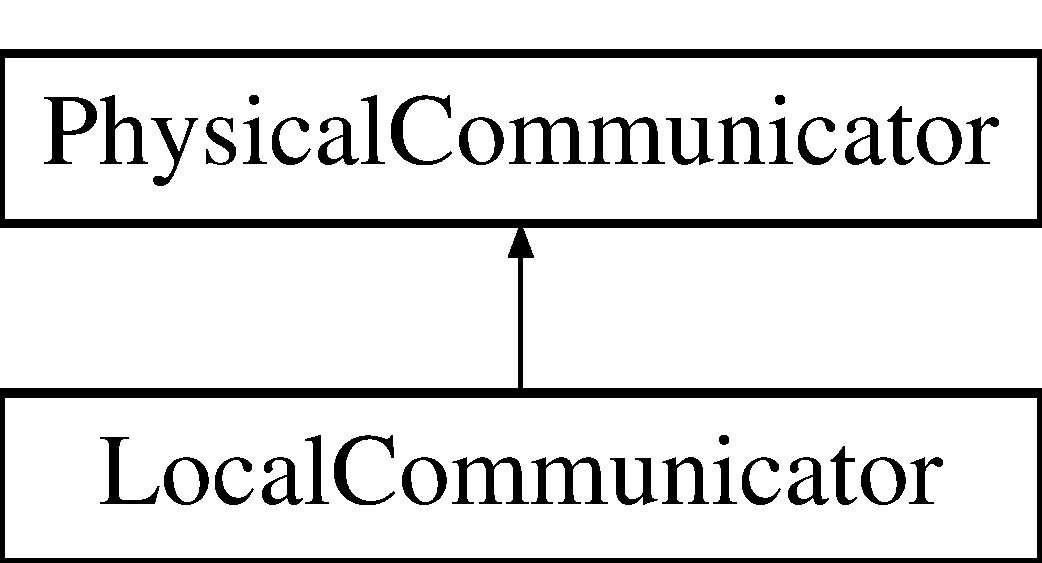
\includegraphics[height=2.000000cm]{classLocalCommunicator}
\end{center}
\end{figure}
\subsection*{Public Member Functions}
\begin{DoxyCompactItemize}
\item 
\hyperlink{classLocalCommunicator_a477260797392154cc43815852ced969c}{Local\+Communicator} (\hyperlink{structcubiumServerSocket__t}{cubium\+Server\+Socket\+\_\+t} $\ast$sock, std\+::shared\+\_\+ptr$<$ \hyperlink{classRoutingTable}{Routing\+Table}$<$ \hyperlink{structcubiumServerSocket__t}{cubium\+Server\+Socket\+\_\+t} $>$$>$ \hyperlink{classLocalCommunicator_ac28392070111396dabbadbbcb81a7ef7}{routing\+Table}, \hyperlink{structLogicalAddress}{Logical\+Address} la)
\item 
\hyperlink{classLocalCommunicator_ac5845882ec445ca5f3bedbaf666073c0}{Local\+Communicator} (\hyperlink{structcubiumClientSocket__t}{cubium\+Client\+Socket\+\_\+t} $\ast$sock, std\+::shared\+\_\+ptr$<$ \hyperlink{classRoutingTable}{Routing\+Table}$<$ \hyperlink{structcubiumServerSocket__t}{cubium\+Server\+Socket\+\_\+t} $>$$>$ \hyperlink{classLocalCommunicator_ac28392070111396dabbadbbcb81a7ef7}{routing\+Table}, \hyperlink{structLogicalAddress}{Logical\+Address} la)
\item 
\hyperlink{classLocalCommunicator_a22dbee26502e3ac2bdf46b9f094d881d}{Local\+Communicator} (\hyperlink{structcubiumServerSocket__t}{cubium\+Server\+Socket\+\_\+t} $\ast$sock, \hyperlink{structLogicalAddress}{Logical\+Address} la)
\item 
virtual bool \hyperlink{classLocalCommunicator_afb8fc8a82069dac7bf08f736fa76c4c8}{send\+Msg} (\hyperlink{structSpaMessage}{Spa\+Message} $\ast$msg, ssize\+\_\+t len)
\item 
virtual void \hyperlink{classLocalCommunicator_a0d6816af83fd55a79990f0b8caa4e164}{handle\+Failure} (std\+::string)
\item 
virtual bool \hyperlink{classLocalCommunicator_a6175c2c35727bb081c5f518e1750dd86}{server\+Send} (\hyperlink{structSpaMessage}{Spa\+Message} $\ast$message, ssize\+\_\+t)
\item 
virtual bool \hyperlink{classLocalCommunicator_afca7f865eda5dca2fc4c3bf5ca697ab8}{client\+Send} (\hyperlink{structSpaMessage}{Spa\+Message} $\ast$message, ssize\+\_\+t)
\item 
void \hyperlink{classLocalCommunicator_a4dc9ea76a7d6d1d363ec8b69c1d5d586}{client\+Connect} (\hyperlink{structSpaMessage}{Spa\+Message} $\ast$, size\+\_\+t, std\+::function$<$ void(\hyperlink{structcubiumClientSocket__t}{cubium\+Client\+Socket\+\_\+t} $\ast$)$>$)
\item 
void \hyperlink{classLocalCommunicator_a8ed10b0a1f9be12597a2e095b7b8fb3e}{init\+Sub\+Dialogue} (\hyperlink{structSpaMessage}{Spa\+Message} $\ast$message, size\+\_\+t len, std\+::function$<$ void(\hyperlink{structcubiumClientSocket__t}{cubium\+Client\+Socket\+\_\+t} $\ast$)$>$ callback)
\item 
void \hyperlink{classLocalCommunicator_a03deedab1d3f79fe328a21aa2d5c6bfb}{client\+Listen} (std\+::function$<$ void(\hyperlink{structcubiumClientSocket__t}{cubium\+Client\+Socket\+\_\+t} $\ast$)$>$)
\item 
virtual void \hyperlink{classLocalCommunicator_a320a09f88a1eb840e517753b603cd08b}{listen} (std\+::function$<$ void(\hyperlink{structcubiumServerSocket__t}{cubium\+Server\+Socket\+\_\+t} $\ast$)$>$)
\item 
virtual void \hyperlink{classLocalCommunicator_a33c7148ee35ec38773b7b4c8f32c643c}{listen} (std\+::function$<$ void(\hyperlink{structcubiumClientSocket__t}{cubium\+Client\+Socket\+\_\+t} $\ast$)$>$)
\item 
void \hyperlink{classLocalCommunicator_a3321b932c8c555587b8b3200bc4dfcdb}{set\+Server\+Sock} (\hyperlink{structcubiumServerSocket__t}{cubium\+Server\+Socket\+\_\+t} $\ast$s)
\item 
void \hyperlink{classLocalCommunicator_a96569a4dc0b07439ab880385428a53f7}{print\+Table} ()
\end{DoxyCompactItemize}
\subsection*{Protected Attributes}
\begin{DoxyCompactItemize}
\item 
\hyperlink{structcubiumServerSocket__t}{cubium\+Server\+Socket\+\_\+t} $\ast$ \hyperlink{classLocalCommunicator_a4c0d8806e53030c1af6124cd55a34335}{server\+Sock}
\item 
\hyperlink{structcubiumClientSocket__t}{cubium\+Client\+Socket\+\_\+t} $\ast$ \hyperlink{classLocalCommunicator_af52bd4819c3dc433bd27d3dbefbaac70}{client\+Sock}
\item 
std\+::shared\+\_\+ptr$<$ \hyperlink{classRoutingTable}{Routing\+Table}$<$ \hyperlink{structcubiumServerSocket__t}{cubium\+Server\+Socket\+\_\+t} $>$ $>$ \hyperlink{classLocalCommunicator_ac28392070111396dabbadbbcb81a7ef7}{routing\+Table}
\end{DoxyCompactItemize}
\subsection*{Additional Inherited Members}


\subsection{Constructor \& Destructor Documentation}
\mbox{\Hypertarget{classLocalCommunicator_a477260797392154cc43815852ced969c}\label{classLocalCommunicator_a477260797392154cc43815852ced969c}} 
\index{Local\+Communicator@{Local\+Communicator}!Local\+Communicator@{Local\+Communicator}}
\index{Local\+Communicator@{Local\+Communicator}!Local\+Communicator@{Local\+Communicator}}
\subsubsection{\texorpdfstring{Local\+Communicator()}{LocalCommunicator()}\hspace{0.1cm}{\footnotesize\ttfamily [1/3]}}
{\footnotesize\ttfamily Local\+Communicator\+::\+Local\+Communicator (\begin{DoxyParamCaption}\item[{\hyperlink{structcubiumServerSocket__t}{cubium\+Server\+Socket\+\_\+t} $\ast$}]{sock,  }\item[{std\+::shared\+\_\+ptr$<$ \hyperlink{classRoutingTable}{Routing\+Table}$<$ \hyperlink{structcubiumServerSocket__t}{cubium\+Server\+Socket\+\_\+t} $>$$>$}]{routing\+Table,  }\item[{\hyperlink{structLogicalAddress}{Logical\+Address}}]{la }\end{DoxyParamCaption})\hspace{0.3cm}{\ttfamily [inline]}}

\mbox{\Hypertarget{classLocalCommunicator_ac5845882ec445ca5f3bedbaf666073c0}\label{classLocalCommunicator_ac5845882ec445ca5f3bedbaf666073c0}} 
\index{Local\+Communicator@{Local\+Communicator}!Local\+Communicator@{Local\+Communicator}}
\index{Local\+Communicator@{Local\+Communicator}!Local\+Communicator@{Local\+Communicator}}
\subsubsection{\texorpdfstring{Local\+Communicator()}{LocalCommunicator()}\hspace{0.1cm}{\footnotesize\ttfamily [2/3]}}
{\footnotesize\ttfamily Local\+Communicator\+::\+Local\+Communicator (\begin{DoxyParamCaption}\item[{\hyperlink{structcubiumClientSocket__t}{cubium\+Client\+Socket\+\_\+t} $\ast$}]{sock,  }\item[{std\+::shared\+\_\+ptr$<$ \hyperlink{classRoutingTable}{Routing\+Table}$<$ \hyperlink{structcubiumServerSocket__t}{cubium\+Server\+Socket\+\_\+t} $>$$>$}]{routing\+Table,  }\item[{\hyperlink{structLogicalAddress}{Logical\+Address}}]{la }\end{DoxyParamCaption})\hspace{0.3cm}{\ttfamily [inline]}}

\mbox{\Hypertarget{classLocalCommunicator_a22dbee26502e3ac2bdf46b9f094d881d}\label{classLocalCommunicator_a22dbee26502e3ac2bdf46b9f094d881d}} 
\index{Local\+Communicator@{Local\+Communicator}!Local\+Communicator@{Local\+Communicator}}
\index{Local\+Communicator@{Local\+Communicator}!Local\+Communicator@{Local\+Communicator}}
\subsubsection{\texorpdfstring{Local\+Communicator()}{LocalCommunicator()}\hspace{0.1cm}{\footnotesize\ttfamily [3/3]}}
{\footnotesize\ttfamily Local\+Communicator\+::\+Local\+Communicator (\begin{DoxyParamCaption}\item[{\hyperlink{structcubiumServerSocket__t}{cubium\+Server\+Socket\+\_\+t} $\ast$}]{sock,  }\item[{\hyperlink{structLogicalAddress}{Logical\+Address}}]{la }\end{DoxyParamCaption})\hspace{0.3cm}{\ttfamily [inline]}}



\subsection{Member Function Documentation}
\mbox{\Hypertarget{classLocalCommunicator_a4dc9ea76a7d6d1d363ec8b69c1d5d586}\label{classLocalCommunicator_a4dc9ea76a7d6d1d363ec8b69c1d5d586}} 
\index{Local\+Communicator@{Local\+Communicator}!client\+Connect@{client\+Connect}}
\index{client\+Connect@{client\+Connect}!Local\+Communicator@{Local\+Communicator}}
\subsubsection{\texorpdfstring{client\+Connect()}{clientConnect()}}
{\footnotesize\ttfamily void Local\+Communicator\+::client\+Connect (\begin{DoxyParamCaption}\item[{\hyperlink{structSpaMessage}{Spa\+Message} $\ast$}]{message,  }\item[{size\+\_\+t}]{len,  }\item[{std\+::function$<$ void(\hyperlink{structcubiumClientSocket__t}{cubium\+Client\+Socket\+\_\+t} $\ast$)$>$}]{callback }\end{DoxyParamCaption})}

\mbox{\Hypertarget{classLocalCommunicator_a03deedab1d3f79fe328a21aa2d5c6bfb}\label{classLocalCommunicator_a03deedab1d3f79fe328a21aa2d5c6bfb}} 
\index{Local\+Communicator@{Local\+Communicator}!client\+Listen@{client\+Listen}}
\index{client\+Listen@{client\+Listen}!Local\+Communicator@{Local\+Communicator}}
\subsubsection{\texorpdfstring{client\+Listen()}{clientListen()}}
{\footnotesize\ttfamily void Local\+Communicator\+::client\+Listen (\begin{DoxyParamCaption}\item[{std\+::function$<$ void(\hyperlink{structcubiumClientSocket__t}{cubium\+Client\+Socket\+\_\+t} $\ast$)$>$}]{func }\end{DoxyParamCaption})}

\mbox{\Hypertarget{classLocalCommunicator_afca7f865eda5dca2fc4c3bf5ca697ab8}\label{classLocalCommunicator_afca7f865eda5dca2fc4c3bf5ca697ab8}} 
\index{Local\+Communicator@{Local\+Communicator}!client\+Send@{client\+Send}}
\index{client\+Send@{client\+Send}!Local\+Communicator@{Local\+Communicator}}
\subsubsection{\texorpdfstring{client\+Send()}{clientSend()}}
{\footnotesize\ttfamily bool Local\+Communicator\+::client\+Send (\begin{DoxyParamCaption}\item[{\hyperlink{structSpaMessage}{Spa\+Message} $\ast$}]{message,  }\item[{ssize\+\_\+t}]{len }\end{DoxyParamCaption})\hspace{0.3cm}{\ttfamily [virtual]}}

\mbox{\Hypertarget{classLocalCommunicator_a0d6816af83fd55a79990f0b8caa4e164}\label{classLocalCommunicator_a0d6816af83fd55a79990f0b8caa4e164}} 
\index{Local\+Communicator@{Local\+Communicator}!handle\+Failure@{handle\+Failure}}
\index{handle\+Failure@{handle\+Failure}!Local\+Communicator@{Local\+Communicator}}
\subsubsection{\texorpdfstring{handle\+Failure()}{handleFailure()}}
{\footnotesize\ttfamily void Local\+Communicator\+::handle\+Failure (\begin{DoxyParamCaption}\item[{std\+::string}]{message }\end{DoxyParamCaption})\hspace{0.3cm}{\ttfamily [virtual]}}

\mbox{\Hypertarget{classLocalCommunicator_a8ed10b0a1f9be12597a2e095b7b8fb3e}\label{classLocalCommunicator_a8ed10b0a1f9be12597a2e095b7b8fb3e}} 
\index{Local\+Communicator@{Local\+Communicator}!init\+Sub\+Dialogue@{init\+Sub\+Dialogue}}
\index{init\+Sub\+Dialogue@{init\+Sub\+Dialogue}!Local\+Communicator@{Local\+Communicator}}
\subsubsection{\texorpdfstring{init\+Sub\+Dialogue()}{initSubDialogue()}}
{\footnotesize\ttfamily void Local\+Communicator\+::init\+Sub\+Dialogue (\begin{DoxyParamCaption}\item[{\hyperlink{structSpaMessage}{Spa\+Message} $\ast$}]{message,  }\item[{size\+\_\+t}]{len,  }\item[{std\+::function$<$ void(\hyperlink{structcubiumClientSocket__t}{cubium\+Client\+Socket\+\_\+t} $\ast$)$>$}]{callback }\end{DoxyParamCaption})}

\mbox{\Hypertarget{classLocalCommunicator_a320a09f88a1eb840e517753b603cd08b}\label{classLocalCommunicator_a320a09f88a1eb840e517753b603cd08b}} 
\index{Local\+Communicator@{Local\+Communicator}!listen@{listen}}
\index{listen@{listen}!Local\+Communicator@{Local\+Communicator}}
\subsubsection{\texorpdfstring{listen()}{listen()}\hspace{0.1cm}{\footnotesize\ttfamily [1/2]}}
{\footnotesize\ttfamily void Local\+Communicator\+::listen (\begin{DoxyParamCaption}\item[{std\+::function$<$ void(\hyperlink{structcubiumServerSocket__t}{cubium\+Server\+Socket\+\_\+t} $\ast$)$>$}]{message\+Handler }\end{DoxyParamCaption})\hspace{0.3cm}{\ttfamily [virtual]}}



Reimplemented from \hyperlink{classPhysicalCommunicator_a4886f4453c1f830ceaef56bc8602423f}{Physical\+Communicator}.

\mbox{\Hypertarget{classLocalCommunicator_a33c7148ee35ec38773b7b4c8f32c643c}\label{classLocalCommunicator_a33c7148ee35ec38773b7b4c8f32c643c}} 
\index{Local\+Communicator@{Local\+Communicator}!listen@{listen}}
\index{listen@{listen}!Local\+Communicator@{Local\+Communicator}}
\subsubsection{\texorpdfstring{listen()}{listen()}\hspace{0.1cm}{\footnotesize\ttfamily [2/2]}}
{\footnotesize\ttfamily void Local\+Communicator\+::listen (\begin{DoxyParamCaption}\item[{std\+::function$<$ void(\hyperlink{structcubiumClientSocket__t}{cubium\+Client\+Socket\+\_\+t} $\ast$)$>$}]{message\+Handler }\end{DoxyParamCaption})\hspace{0.3cm}{\ttfamily [virtual]}}

\mbox{\Hypertarget{classLocalCommunicator_a96569a4dc0b07439ab880385428a53f7}\label{classLocalCommunicator_a96569a4dc0b07439ab880385428a53f7}} 
\index{Local\+Communicator@{Local\+Communicator}!print\+Table@{print\+Table}}
\index{print\+Table@{print\+Table}!Local\+Communicator@{Local\+Communicator}}
\subsubsection{\texorpdfstring{print\+Table()}{printTable()}}
{\footnotesize\ttfamily void Local\+Communicator\+::print\+Table (\begin{DoxyParamCaption}{ }\end{DoxyParamCaption})\hspace{0.3cm}{\ttfamily [inline]}}

\mbox{\Hypertarget{classLocalCommunicator_afb8fc8a82069dac7bf08f736fa76c4c8}\label{classLocalCommunicator_afb8fc8a82069dac7bf08f736fa76c4c8}} 
\index{Local\+Communicator@{Local\+Communicator}!send\+Msg@{send\+Msg}}
\index{send\+Msg@{send\+Msg}!Local\+Communicator@{Local\+Communicator}}
\subsubsection{\texorpdfstring{send\+Msg()}{sendMsg()}}
{\footnotesize\ttfamily bool Local\+Communicator\+::send\+Msg (\begin{DoxyParamCaption}\item[{\hyperlink{structSpaMessage}{Spa\+Message} $\ast$}]{msg,  }\item[{ssize\+\_\+t}]{len }\end{DoxyParamCaption})\hspace{0.3cm}{\ttfamily [virtual]}}



Reimplemented from \hyperlink{classPhysicalCommunicator_a9fc5595b693f9908a20d0e64a6579bb5}{Physical\+Communicator}.

\mbox{\Hypertarget{classLocalCommunicator_a6175c2c35727bb081c5f518e1750dd86}\label{classLocalCommunicator_a6175c2c35727bb081c5f518e1750dd86}} 
\index{Local\+Communicator@{Local\+Communicator}!server\+Send@{server\+Send}}
\index{server\+Send@{server\+Send}!Local\+Communicator@{Local\+Communicator}}
\subsubsection{\texorpdfstring{server\+Send()}{serverSend()}}
{\footnotesize\ttfamily bool Local\+Communicator\+::server\+Send (\begin{DoxyParamCaption}\item[{\hyperlink{structSpaMessage}{Spa\+Message} $\ast$}]{message,  }\item[{ssize\+\_\+t}]{len }\end{DoxyParamCaption})\hspace{0.3cm}{\ttfamily [virtual]}}

\mbox{\Hypertarget{classLocalCommunicator_a3321b932c8c555587b8b3200bc4dfcdb}\label{classLocalCommunicator_a3321b932c8c555587b8b3200bc4dfcdb}} 
\index{Local\+Communicator@{Local\+Communicator}!set\+Server\+Sock@{set\+Server\+Sock}}
\index{set\+Server\+Sock@{set\+Server\+Sock}!Local\+Communicator@{Local\+Communicator}}
\subsubsection{\texorpdfstring{set\+Server\+Sock()}{setServerSock()}}
{\footnotesize\ttfamily void Local\+Communicator\+::set\+Server\+Sock (\begin{DoxyParamCaption}\item[{\hyperlink{structcubiumServerSocket__t}{cubium\+Server\+Socket\+\_\+t} $\ast$}]{s }\end{DoxyParamCaption})\hspace{0.3cm}{\ttfamily [inline]}}



\subsection{Member Data Documentation}
\mbox{\Hypertarget{classLocalCommunicator_af52bd4819c3dc433bd27d3dbefbaac70}\label{classLocalCommunicator_af52bd4819c3dc433bd27d3dbefbaac70}} 
\index{Local\+Communicator@{Local\+Communicator}!client\+Sock@{client\+Sock}}
\index{client\+Sock@{client\+Sock}!Local\+Communicator@{Local\+Communicator}}
\subsubsection{\texorpdfstring{client\+Sock}{clientSock}}
{\footnotesize\ttfamily \hyperlink{structcubiumClientSocket__t}{cubium\+Client\+Socket\+\_\+t}$\ast$ Local\+Communicator\+::client\+Sock\hspace{0.3cm}{\ttfamily [protected]}}

\mbox{\Hypertarget{classLocalCommunicator_ac28392070111396dabbadbbcb81a7ef7}\label{classLocalCommunicator_ac28392070111396dabbadbbcb81a7ef7}} 
\index{Local\+Communicator@{Local\+Communicator}!routing\+Table@{routing\+Table}}
\index{routing\+Table@{routing\+Table}!Local\+Communicator@{Local\+Communicator}}
\subsubsection{\texorpdfstring{routing\+Table}{routingTable}}
{\footnotesize\ttfamily std\+::shared\+\_\+ptr$<$\hyperlink{classRoutingTable}{Routing\+Table}$<$\hyperlink{structcubiumServerSocket__t}{cubium\+Server\+Socket\+\_\+t}$>$ $>$ Local\+Communicator\+::routing\+Table\hspace{0.3cm}{\ttfamily [protected]}}

\mbox{\Hypertarget{classLocalCommunicator_a4c0d8806e53030c1af6124cd55a34335}\label{classLocalCommunicator_a4c0d8806e53030c1af6124cd55a34335}} 
\index{Local\+Communicator@{Local\+Communicator}!server\+Sock@{server\+Sock}}
\index{server\+Sock@{server\+Sock}!Local\+Communicator@{Local\+Communicator}}
\subsubsection{\texorpdfstring{server\+Sock}{serverSock}}
{\footnotesize\ttfamily \hyperlink{structcubiumServerSocket__t}{cubium\+Server\+Socket\+\_\+t}$\ast$ Local\+Communicator\+::server\+Sock\hspace{0.3cm}{\ttfamily [protected]}}



The documentation for this class was generated from the following files\+:\begin{DoxyCompactItemize}
\item 
lib/\hyperlink{local__communicator_8hpp}{local\+\_\+communicator.\+hpp}\item 
lib/\hyperlink{local__communicator_8cpp}{local\+\_\+communicator.\+cpp}\end{DoxyCompactItemize}

\hypertarget{structLocalHello}{}\section{Local\+Hello Struct Reference}
\label{structLocalHello}\index{Local\+Hello@{Local\+Hello}}
\subsection*{Public Member Functions}
\begin{DoxyCompactItemize}
\item 
\mbox{\Hypertarget{structLocalHello_a2ea0d07ccd8786604938da56efaa3144}\label{structLocalHello_a2ea0d07ccd8786604938da56efaa3144}} 
{\bfseries Local\+Hello} (uint8\+\_\+t version, uint8\+\_\+t priority, \hyperlink{structLogicalAddress}{Logical\+Address} destination, \hyperlink{structLogicalAddress}{Logical\+Address} source, uint16\+\_\+t flags, uint16\+\_\+t source\+Port, uint64\+\_\+t uuid, uint8\+\_\+t component\+Type)
\end{DoxyCompactItemize}
\subsection*{Public Attributes}
\begin{DoxyCompactItemize}
\item 
\mbox{\Hypertarget{structLocalHello_a89f32f528654b416a69c06083fa2c326}\label{structLocalHello_a89f32f528654b416a69c06083fa2c326}} 
\hyperlink{structLocalSpaMessage}{Local\+Spa\+Message} {\bfseries local\+Spa\+Message}
\item 
\mbox{\Hypertarget{structLocalHello_a2793976cc1bea077237bb17c2dbb1713}\label{structLocalHello_a2793976cc1bea077237bb17c2dbb1713}} 
uint64\+\_\+t {\bfseries uuid}
\item 
\mbox{\Hypertarget{structLocalHello_a1814191cf0ab5e8b281ff3d3f2b455cc}\label{structLocalHello_a1814191cf0ab5e8b281ff3d3f2b455cc}} 
uint8\+\_\+t {\bfseries component\+Type}
\end{DoxyCompactItemize}


The documentation for this struct was generated from the following file\+:\begin{DoxyCompactItemize}
\item 
lib/messages/local/local\+\_\+hello.\+h\end{DoxyCompactItemize}

\hypertarget{structLocalSpaMessage}{}\section{Local\+Spa\+Message Struct Reference}
\label{structLocalSpaMessage}\index{Local\+Spa\+Message@{Local\+Spa\+Message}}
\subsection*{Public Member Functions}
\begin{DoxyCompactItemize}
\item 
\mbox{\Hypertarget{structLocalSpaMessage_a3d0882edfa48a1604ec30784308d65d6}\label{structLocalSpaMessage_a3d0882edfa48a1604ec30784308d65d6}} 
{\bfseries Local\+Spa\+Message} (uint8\+\_\+t version, uint8\+\_\+t priority, uint16\+\_\+t length, \hyperlink{structLogicalAddress}{Logical\+Address} destination, \hyperlink{structLogicalAddress}{Logical\+Address} source, uint16\+\_\+t flags, uint8\+\_\+t opcode, uint16\+\_\+t source\+Port)
\end{DoxyCompactItemize}
\subsection*{Public Attributes}
\begin{DoxyCompactItemize}
\item 
\mbox{\Hypertarget{structLocalSpaMessage_a87829228c5af1850fc3efc288cfbbdfc}\label{structLocalSpaMessage_a87829228c5af1850fc3efc288cfbbdfc}} 
\hyperlink{structSpaMessage}{Spa\+Message} {\bfseries spa\+Message}
\item 
\mbox{\Hypertarget{structLocalSpaMessage_af8cc4ca1b9f7d7d993b563e0110e940a}\label{structLocalSpaMessage_af8cc4ca1b9f7d7d993b563e0110e940a}} 
\hyperlink{structSpaLocalHeader}{Spa\+Local\+Header} {\bfseries spa\+Local\+Header}
\end{DoxyCompactItemize}


The documentation for this struct was generated from the following file\+:\begin{DoxyCompactItemize}
\item 
lib/messages/local/local\+\_\+spa\+\_\+message.\+h\end{DoxyCompactItemize}

\hypertarget{classLocalSubnetManager}{}\section{Local\+Subnet\+Manager Class Reference}
\label{classLocalSubnetManager}\index{Local\+Subnet\+Manager@{Local\+Subnet\+Manager}}


{\ttfamily \#include $<$local\+\_\+subnet\+\_\+manager.\+hpp$>$}

Inheritance diagram for Local\+Subnet\+Manager\+:\begin{figure}[H]
\begin{center}
\leavevmode
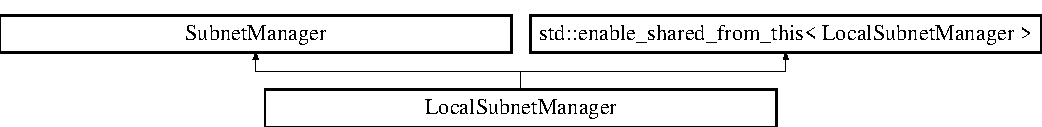
\includegraphics[height=1.702128cm]{classLocalSubnetManager}
\end{center}
\end{figure}
\subsection*{Public Member Functions}
\begin{DoxyCompactItemize}
\item 
\hyperlink{classLocalSubnetManager_ae77d1c9d08c317f43e7a36d1ae8671f3}{Local\+Subnet\+Manager} (std\+::shared\+\_\+ptr$<$ \hyperlink{classSpaCommunicator}{Spa\+Communicator} $>$ c, std\+::shared\+\_\+ptr$<$ \hyperlink{classRoutingTable}{Routing\+Table}$<$ \hyperlink{structcubiumServerSocket__t}{cubium\+Server\+Socket\+\_\+t} $>$$>$ rt)
\item 
void \hyperlink{classLocalSubnetManager_a8cd2838196edcd75a77f532bce15c2fd}{listen\+Messages} ()
\item 
void \hyperlink{classLocalSubnetManager_a6eb06d8e5e5c3ae23552e3cde0f4c216}{receive\+Message} (\hyperlink{structSpaMessage}{Spa\+Message} $\ast$message)
\end{DoxyCompactItemize}
\subsection*{Private Attributes}
\begin{DoxyCompactItemize}
\item 
\hyperlink{classComponentList}{Component\+List} \hyperlink{classLocalSubnetManager_abc353dea714fbebbcd5dd37fab411299}{components}
\item 
std\+::shared\+\_\+ptr$<$ \hyperlink{classRoutingTable}{Routing\+Table}$<$ \hyperlink{structcubiumServerSocket__t}{cubium\+Server\+Socket\+\_\+t} $>$ $>$ \hyperlink{classLocalSubnetManager_afbdea942383e01998f54098eb157d89c}{routing\+Table}
\end{DoxyCompactItemize}
\subsection*{Friends}
\begin{DoxyCompactItemize}
\item 
void \hyperlink{classLocalSubnetManager_a15ed1b4951854aeb9f6bdd54816a16be}{L\+S\+M\+\_\+message\+Callback} (std\+::shared\+\_\+ptr$<$ \hyperlink{classLocalSubnetManager}{Local\+Subnet\+Manager} $>$ lsm, \hyperlink{structcubiumServerSocket__t}{cubium\+Server\+Socket\+\_\+t} $\ast$sock)
\end{DoxyCompactItemize}
\subsection*{Additional Inherited Members}


\subsection{Constructor \& Destructor Documentation}
\mbox{\Hypertarget{classLocalSubnetManager_ae77d1c9d08c317f43e7a36d1ae8671f3}\label{classLocalSubnetManager_ae77d1c9d08c317f43e7a36d1ae8671f3}} 
\index{Local\+Subnet\+Manager@{Local\+Subnet\+Manager}!Local\+Subnet\+Manager@{Local\+Subnet\+Manager}}
\index{Local\+Subnet\+Manager@{Local\+Subnet\+Manager}!Local\+Subnet\+Manager@{Local\+Subnet\+Manager}}
\subsubsection{\texorpdfstring{Local\+Subnet\+Manager()}{LocalSubnetManager()}}
{\footnotesize\ttfamily Local\+Subnet\+Manager\+::\+Local\+Subnet\+Manager (\begin{DoxyParamCaption}\item[{std\+::shared\+\_\+ptr$<$ \hyperlink{classSpaCommunicator}{Spa\+Communicator} $>$}]{c,  }\item[{std\+::shared\+\_\+ptr$<$ \hyperlink{classRoutingTable}{Routing\+Table}$<$ \hyperlink{structcubiumServerSocket__t}{cubium\+Server\+Socket\+\_\+t} $>$$>$}]{rt }\end{DoxyParamCaption})\hspace{0.3cm}{\ttfamily [inline]}}



\subsection{Member Function Documentation}
\mbox{\Hypertarget{classLocalSubnetManager_a8cd2838196edcd75a77f532bce15c2fd}\label{classLocalSubnetManager_a8cd2838196edcd75a77f532bce15c2fd}} 
\index{Local\+Subnet\+Manager@{Local\+Subnet\+Manager}!listen\+Messages@{listen\+Messages}}
\index{listen\+Messages@{listen\+Messages}!Local\+Subnet\+Manager@{Local\+Subnet\+Manager}}
\subsubsection{\texorpdfstring{listen\+Messages()}{listenMessages()}}
{\footnotesize\ttfamily void Local\+Subnet\+Manager\+::listen\+Messages (\begin{DoxyParamCaption}{ }\end{DoxyParamCaption})\hspace{0.3cm}{\ttfamily [inline]}, {\ttfamily [virtual]}}


\begin{DoxyParams}{Parameters}
{\em message} & -\/ message that has been received Continuously ping components checking to make sure they are still responsive. Should report component failture to logging service. This function should not return while the subnet manager is running. Continuously listen for messages. Will call receive\+Message with each received message. A call to this method should not return while the subnet manager is running. \\
\hline
\end{DoxyParams}


Implements \hyperlink{classSubnetManager_a6aed1acaa5e9f18feb7667904675d119}{Subnet\+Manager}.

\mbox{\Hypertarget{classLocalSubnetManager_a6eb06d8e5e5c3ae23552e3cde0f4c216}\label{classLocalSubnetManager_a6eb06d8e5e5c3ae23552e3cde0f4c216}} 
\index{Local\+Subnet\+Manager@{Local\+Subnet\+Manager}!receive\+Message@{receive\+Message}}
\index{receive\+Message@{receive\+Message}!Local\+Subnet\+Manager@{Local\+Subnet\+Manager}}
\subsubsection{\texorpdfstring{receive\+Message()}{receiveMessage()}}
{\footnotesize\ttfamily void Local\+Subnet\+Manager\+::receive\+Message (\begin{DoxyParamCaption}\item[{\hyperlink{structSpaMessage}{Spa\+Message} $\ast$}]{message }\end{DoxyParamCaption})\hspace{0.3cm}{\ttfamily [inline]}}



\subsection{Friends And Related Function Documentation}
\mbox{\Hypertarget{classLocalSubnetManager_a15ed1b4951854aeb9f6bdd54816a16be}\label{classLocalSubnetManager_a15ed1b4951854aeb9f6bdd54816a16be}} 
\index{Local\+Subnet\+Manager@{Local\+Subnet\+Manager}!L\+S\+M\+\_\+message\+Callback@{L\+S\+M\+\_\+message\+Callback}}
\index{L\+S\+M\+\_\+message\+Callback@{L\+S\+M\+\_\+message\+Callback}!Local\+Subnet\+Manager@{Local\+Subnet\+Manager}}
\subsubsection{\texorpdfstring{L\+S\+M\+\_\+message\+Callback}{LSM\_messageCallback}}
{\footnotesize\ttfamily void L\+S\+M\+\_\+message\+Callback (\begin{DoxyParamCaption}\item[{std\+::shared\+\_\+ptr$<$ \hyperlink{classLocalSubnetManager}{Local\+Subnet\+Manager} $>$}]{lsm,  }\item[{\hyperlink{structcubiumServerSocket__t}{cubium\+Server\+Socket\+\_\+t} $\ast$}]{sock }\end{DoxyParamCaption})\hspace{0.3cm}{\ttfamily [friend]}}



\subsection{Member Data Documentation}
\mbox{\Hypertarget{classLocalSubnetManager_abc353dea714fbebbcd5dd37fab411299}\label{classLocalSubnetManager_abc353dea714fbebbcd5dd37fab411299}} 
\index{Local\+Subnet\+Manager@{Local\+Subnet\+Manager}!components@{components}}
\index{components@{components}!Local\+Subnet\+Manager@{Local\+Subnet\+Manager}}
\subsubsection{\texorpdfstring{components}{components}}
{\footnotesize\ttfamily \hyperlink{classComponentList}{Component\+List} Local\+Subnet\+Manager\+::components\hspace{0.3cm}{\ttfamily [private]}}

\mbox{\Hypertarget{classLocalSubnetManager_afbdea942383e01998f54098eb157d89c}\label{classLocalSubnetManager_afbdea942383e01998f54098eb157d89c}} 
\index{Local\+Subnet\+Manager@{Local\+Subnet\+Manager}!routing\+Table@{routing\+Table}}
\index{routing\+Table@{routing\+Table}!Local\+Subnet\+Manager@{Local\+Subnet\+Manager}}
\subsubsection{\texorpdfstring{routing\+Table}{routingTable}}
{\footnotesize\ttfamily std\+::shared\+\_\+ptr$<$\hyperlink{classRoutingTable}{Routing\+Table}$<$\hyperlink{structcubiumServerSocket__t}{cubium\+Server\+Socket\+\_\+t}$>$ $>$ Local\+Subnet\+Manager\+::routing\+Table\hspace{0.3cm}{\ttfamily [private]}}



The documentation for this class was generated from the following file\+:\begin{DoxyCompactItemize}
\item 
lib/\hyperlink{local__subnet__manager_8hpp}{local\+\_\+subnet\+\_\+manager.\+hpp}\end{DoxyCompactItemize}

\hypertarget{structLogicalAddress}{}\section{Logical\+Address Struct Reference}
\label{structLogicalAddress}\index{Logical\+Address@{Logical\+Address}}
\subsection*{Public Member Functions}
\begin{DoxyCompactItemize}
\item 
\mbox{\Hypertarget{structLogicalAddress_a5ca025d24b9b8e2925814d3fc6607bd4}\label{structLogicalAddress_a5ca025d24b9b8e2925814d3fc6607bd4}} 
{\bfseries Logical\+Address} (uint16\+\_\+t sub\+Id=0, uint16\+\_\+t comp\+Id=0)
\item 
\mbox{\Hypertarget{structLogicalAddress_a9a8483eda7a165e0413a5b7334e47fc8}\label{structLogicalAddress_a9a8483eda7a165e0413a5b7334e47fc8}} 
bool {\bfseries is\+On\+Same\+Subnet} (\hyperlink{structLogicalAddress}{Logical\+Address} other)
\end{DoxyCompactItemize}
\subsection*{Public Attributes}
\begin{DoxyCompactItemize}
\item 
\mbox{\Hypertarget{structLogicalAddress_a2ea7e86b6587adbfe03b16c7e0f0fe3b}\label{structLogicalAddress_a2ea7e86b6587adbfe03b16c7e0f0fe3b}} 
uint16\+\_\+t {\bfseries subnet\+Id}
\item 
\mbox{\Hypertarget{structLogicalAddress_ac4f97357841656cd45f3183630b7af45}\label{structLogicalAddress_ac4f97357841656cd45f3183630b7af45}} 
uint16\+\_\+t {\bfseries component\+Id}
\end{DoxyCompactItemize}


The documentation for this struct was generated from the following file\+:\begin{DoxyCompactItemize}
\item 
lib/logical\+\_\+address.\+h\end{DoxyCompactItemize}

\hypertarget{structLogicalAddressCompare}{}\section{Logical\+Address\+Compare Struct Reference}
\label{structLogicalAddressCompare}\index{Logical\+Address\+Compare@{Logical\+Address\+Compare}}


{\ttfamily \#include $<$logical\+\_\+address.\+h$>$}

\subsection*{Public Member Functions}
\begin{DoxyCompactItemize}
\item 
bool \hyperlink{structLogicalAddressCompare_aa509931ff644dc8f60f77467d7d76a3c}{operator()} (const \hyperlink{structLogicalAddress}{Logical\+Address} \&lhs, const \hyperlink{structLogicalAddress}{Logical\+Address} \&rhs) const
\end{DoxyCompactItemize}


\subsection{Member Function Documentation}
\mbox{\Hypertarget{structLogicalAddressCompare_aa509931ff644dc8f60f77467d7d76a3c}\label{structLogicalAddressCompare_aa509931ff644dc8f60f77467d7d76a3c}} 
\index{Logical\+Address\+Compare@{Logical\+Address\+Compare}!operator()@{operator()}}
\index{operator()@{operator()}!Logical\+Address\+Compare@{Logical\+Address\+Compare}}
\subsubsection{\texorpdfstring{operator()()}{operator()()}}
{\footnotesize\ttfamily bool Logical\+Address\+Compare\+::operator() (\begin{DoxyParamCaption}\item[{const \hyperlink{structLogicalAddress}{Logical\+Address} \&}]{lhs,  }\item[{const \hyperlink{structLogicalAddress}{Logical\+Address} \&}]{rhs }\end{DoxyParamCaption}) const\hspace{0.3cm}{\ttfamily [inline]}}



The documentation for this struct was generated from the following file\+:\begin{DoxyCompactItemize}
\item 
lib/\hyperlink{logical__address_8h}{logical\+\_\+address.\+h}\end{DoxyCompactItemize}

\hypertarget{classAdafruit__MCP9808_1_1MCP9808_1_1MCP9808}{}\section{Adafruit\+\_\+\+M\+C\+P9808.\+M\+C\+P9808.\+M\+C\+P9808 Class Reference}
\label{classAdafruit__MCP9808_1_1MCP9808_1_1MCP9808}\index{Adafruit\+\_\+\+M\+C\+P9808.\+M\+C\+P9808.\+M\+C\+P9808@{Adafruit\+\_\+\+M\+C\+P9808.\+M\+C\+P9808.\+M\+C\+P9808}}
Inheritance diagram for Adafruit\+\_\+\+M\+C\+P9808.\+M\+C\+P9808.\+M\+C\+P9808\+:\begin{figure}[H]
\begin{center}
\leavevmode
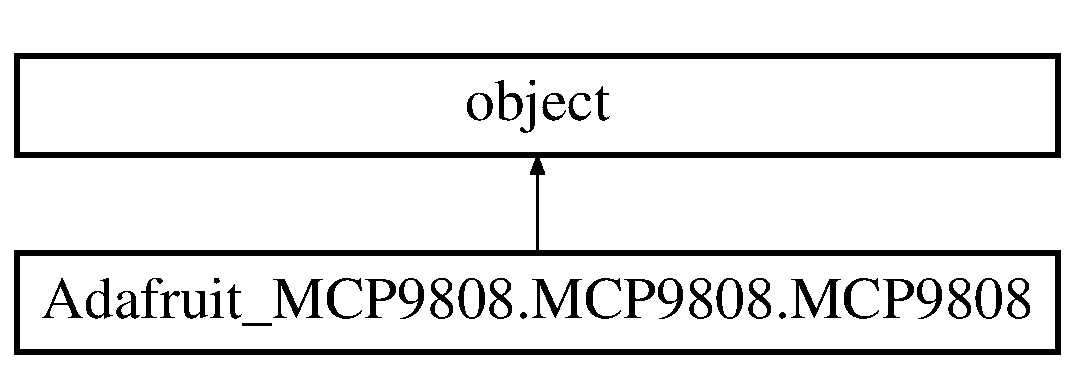
\includegraphics[height=2.000000cm]{classAdafruit__MCP9808_1_1MCP9808_1_1MCP9808}
\end{center}
\end{figure}
\subsection*{Public Member Functions}
\begin{DoxyCompactItemize}
\item 
def \hyperlink{classAdafruit__MCP9808_1_1MCP9808_1_1MCP9808_a6c7c1f671a5a3224bb7e081ea5811d06}{\+\_\+\+\_\+init\+\_\+\+\_\+} (self, address=M\+C\+P9808\+\_\+\+I2\+C\+A\+D\+D\+R\+\_\+\+D\+E\+F\+A\+U\+LT, i2c=None, kwargs)
\item 
def \hyperlink{classAdafruit__MCP9808_1_1MCP9808_1_1MCP9808_ab62a703ef4cf09887846d3eeaa401772}{begin} (self)
\item 
def \hyperlink{classAdafruit__MCP9808_1_1MCP9808_1_1MCP9808_a0920c36ee50223d2fda4f6e7caadcada}{read\+TempC} (self)
\end{DoxyCompactItemize}


\subsection{Detailed Description}
\begin{DoxyVerb}Class to represent an Adafruit MCP9808 precision temperature measurement
board.
\end{DoxyVerb}
 

\subsection{Constructor \& Destructor Documentation}
\mbox{\Hypertarget{classAdafruit__MCP9808_1_1MCP9808_1_1MCP9808_a6c7c1f671a5a3224bb7e081ea5811d06}\label{classAdafruit__MCP9808_1_1MCP9808_1_1MCP9808_a6c7c1f671a5a3224bb7e081ea5811d06}} 
\index{Adafruit\+\_\+\+M\+C\+P9808\+::\+M\+C\+P9808\+::\+M\+C\+P9808@{Adafruit\+\_\+\+M\+C\+P9808\+::\+M\+C\+P9808\+::\+M\+C\+P9808}!\+\_\+\+\_\+init\+\_\+\+\_\+@{\+\_\+\+\_\+init\+\_\+\+\_\+}}
\index{\+\_\+\+\_\+init\+\_\+\+\_\+@{\+\_\+\+\_\+init\+\_\+\+\_\+}!Adafruit\+\_\+\+M\+C\+P9808\+::\+M\+C\+P9808\+::\+M\+C\+P9808@{Adafruit\+\_\+\+M\+C\+P9808\+::\+M\+C\+P9808\+::\+M\+C\+P9808}}
\subsubsection{\texorpdfstring{\+\_\+\+\_\+init\+\_\+\+\_\+()}{\_\_init\_\_()}}
{\footnotesize\ttfamily def Adafruit\+\_\+\+M\+C\+P9808.\+M\+C\+P9808.\+M\+C\+P9808.\+\_\+\+\_\+init\+\_\+\+\_\+ (\begin{DoxyParamCaption}\item[{}]{self,  }\item[{}]{address = {\ttfamily MCP9808\+\_\+I2CADDR\+\_\+DEFAULT},  }\item[{}]{i2c = {\ttfamily None},  }\item[{}]{kwargs }\end{DoxyParamCaption})}

\begin{DoxyVerb}Initialize MCP9808 device on the specified I2C address and bus number.
Address defaults to 0x18 and bus number defaults to the appropriate bus
for the hardware.
\end{DoxyVerb}
 

\subsection{Member Function Documentation}
\mbox{\Hypertarget{classAdafruit__MCP9808_1_1MCP9808_1_1MCP9808_ab62a703ef4cf09887846d3eeaa401772}\label{classAdafruit__MCP9808_1_1MCP9808_1_1MCP9808_ab62a703ef4cf09887846d3eeaa401772}} 
\index{Adafruit\+\_\+\+M\+C\+P9808\+::\+M\+C\+P9808\+::\+M\+C\+P9808@{Adafruit\+\_\+\+M\+C\+P9808\+::\+M\+C\+P9808\+::\+M\+C\+P9808}!begin@{begin}}
\index{begin@{begin}!Adafruit\+\_\+\+M\+C\+P9808\+::\+M\+C\+P9808\+::\+M\+C\+P9808@{Adafruit\+\_\+\+M\+C\+P9808\+::\+M\+C\+P9808\+::\+M\+C\+P9808}}
\subsubsection{\texorpdfstring{begin()}{begin()}}
{\footnotesize\ttfamily def Adafruit\+\_\+\+M\+C\+P9808.\+M\+C\+P9808.\+M\+C\+P9808.\+begin (\begin{DoxyParamCaption}\item[{}]{self }\end{DoxyParamCaption})}

\begin{DoxyVerb}Start taking temperature measurements. Returns True if the device is 
intialized, False otherwise.
\end{DoxyVerb}
 \mbox{\Hypertarget{classAdafruit__MCP9808_1_1MCP9808_1_1MCP9808_a0920c36ee50223d2fda4f6e7caadcada}\label{classAdafruit__MCP9808_1_1MCP9808_1_1MCP9808_a0920c36ee50223d2fda4f6e7caadcada}} 
\index{Adafruit\+\_\+\+M\+C\+P9808\+::\+M\+C\+P9808\+::\+M\+C\+P9808@{Adafruit\+\_\+\+M\+C\+P9808\+::\+M\+C\+P9808\+::\+M\+C\+P9808}!read\+TempC@{read\+TempC}}
\index{read\+TempC@{read\+TempC}!Adafruit\+\_\+\+M\+C\+P9808\+::\+M\+C\+P9808\+::\+M\+C\+P9808@{Adafruit\+\_\+\+M\+C\+P9808\+::\+M\+C\+P9808\+::\+M\+C\+P9808}}
\subsubsection{\texorpdfstring{read\+Temp\+C()}{readTempC()}}
{\footnotesize\ttfamily def Adafruit\+\_\+\+M\+C\+P9808.\+M\+C\+P9808.\+M\+C\+P9808.\+read\+TempC (\begin{DoxyParamCaption}\item[{}]{self }\end{DoxyParamCaption})}

\begin{DoxyVerb}Read sensor and return its value in degrees celsius.\end{DoxyVerb}
 

The documentation for this class was generated from the following file\+:\begin{DoxyCompactItemize}
\item 
drivers/\+Temp\+Sensor/\+Adafruit\+\_\+\+Python\+\_\+\+M\+C\+P9808/\+Adafruit\+\_\+\+M\+C\+P9808/M\+C\+P9808.\+py\end{DoxyCompactItemize}

\hypertarget{classPhysicalCommunicator}{}\section{Physical\+Communicator Class Reference}
\label{classPhysicalCommunicator}\index{Physical\+Communicator@{Physical\+Communicator}}


{\ttfamily \#include $<$physical\+\_\+communicator.\+hpp$>$}

Inheritance diagram for Physical\+Communicator\+:\begin{figure}[H]
\begin{center}
\leavevmode
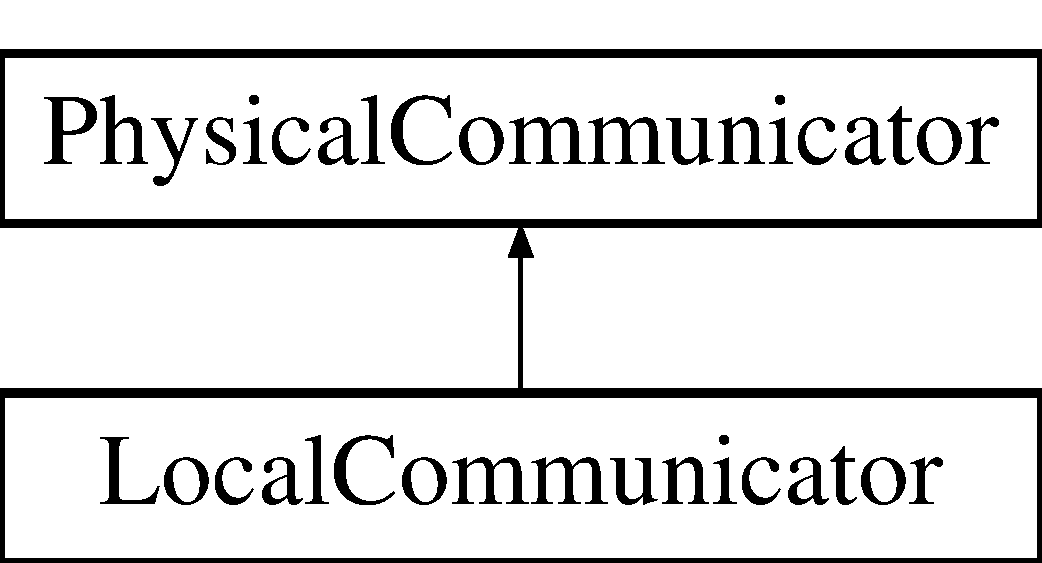
\includegraphics[height=2.000000cm]{classPhysicalCommunicator}
\end{center}
\end{figure}
\subsection*{Public Types}
\begin{DoxyCompactItemize}
\item 
typedef void($\ast$ \hyperlink{classPhysicalCommunicator_ac0fb9cea7a3e3ffecedc57be9684ebbf}{Message\+Callback}) (void $\ast$, uint32\+\_\+t)
\end{DoxyCompactItemize}
\subsection*{Public Member Functions}
\begin{DoxyCompactItemize}
\item 
\hyperlink{classPhysicalCommunicator_a6895d0ce73240eb80d0b9a060da7c728}{Physical\+Communicator} (\hyperlink{structLogicalAddress}{Logical\+Address} la)
\item 
virtual \hyperlink{classPhysicalCommunicator_ab81e6bd21e71a33a5835c16e74ffd324}{$\sim$\+Physical\+Communicator} ()
\item 
virtual bool \hyperlink{classPhysicalCommunicator_a9fc5595b693f9908a20d0e64a6579bb5}{send\+Msg} (\hyperlink{structSpaMessage}{Spa\+Message} $\ast$message, ssize\+\_\+t len)
\item 
virtual void \hyperlink{classPhysicalCommunicator_a4886f4453c1f830ceaef56bc8602423f}{listen} (std\+::function$<$ void(\hyperlink{structcubiumServerSocket__t}{cubium\+Server\+Socket\+\_\+t} $\ast$)$>$)
\item 
virtual \hyperlink{structLogicalAddress}{Logical\+Address} \hyperlink{classPhysicalCommunicator_a80f3bdf1beb61e5f6721e30fdc4d5d7f}{get\+Subnet\+Address} ()
\item 
virtual void \hyperlink{classPhysicalCommunicator_a5984183c86e19370215736688d905fe6}{client\+Connect} (\hyperlink{structSpaMessage}{Spa\+Message} $\ast$, std\+::function$<$ void(\hyperlink{structcubiumClientSocket__t}{cubium\+Client\+Socket\+\_\+t} $\ast$)$>$)
\end{DoxyCompactItemize}
\subsection*{Public Attributes}
\begin{DoxyCompactItemize}
\item 
\hyperlink{structLogicalAddress}{Logical\+Address} \hyperlink{classPhysicalCommunicator_a2ed89508db3fe68218192a6f3bacab26}{subnet\+Address}
\end{DoxyCompactItemize}


\subsection{Member Typedef Documentation}
\mbox{\Hypertarget{classPhysicalCommunicator_ac0fb9cea7a3e3ffecedc57be9684ebbf}\label{classPhysicalCommunicator_ac0fb9cea7a3e3ffecedc57be9684ebbf}} 
\index{Physical\+Communicator@{Physical\+Communicator}!Message\+Callback@{Message\+Callback}}
\index{Message\+Callback@{Message\+Callback}!Physical\+Communicator@{Physical\+Communicator}}
\subsubsection{\texorpdfstring{Message\+Callback}{MessageCallback}}
{\footnotesize\ttfamily typedef void($\ast$ Physical\+Communicator\+::\+Message\+Callback) (void $\ast$, uint32\+\_\+t)}



\subsection{Constructor \& Destructor Documentation}
\mbox{\Hypertarget{classPhysicalCommunicator_a6895d0ce73240eb80d0b9a060da7c728}\label{classPhysicalCommunicator_a6895d0ce73240eb80d0b9a060da7c728}} 
\index{Physical\+Communicator@{Physical\+Communicator}!Physical\+Communicator@{Physical\+Communicator}}
\index{Physical\+Communicator@{Physical\+Communicator}!Physical\+Communicator@{Physical\+Communicator}}
\subsubsection{\texorpdfstring{Physical\+Communicator()}{PhysicalCommunicator()}}
{\footnotesize\ttfamily Physical\+Communicator\+::\+Physical\+Communicator (\begin{DoxyParamCaption}\item[{\hyperlink{structLogicalAddress}{Logical\+Address}}]{la }\end{DoxyParamCaption})\hspace{0.3cm}{\ttfamily [inline]}}

\mbox{\Hypertarget{classPhysicalCommunicator_ab81e6bd21e71a33a5835c16e74ffd324}\label{classPhysicalCommunicator_ab81e6bd21e71a33a5835c16e74ffd324}} 
\index{Physical\+Communicator@{Physical\+Communicator}!````~Physical\+Communicator@{$\sim$\+Physical\+Communicator}}
\index{````~Physical\+Communicator@{$\sim$\+Physical\+Communicator}!Physical\+Communicator@{Physical\+Communicator}}
\subsubsection{\texorpdfstring{$\sim$\+Physical\+Communicator()}{~PhysicalCommunicator()}}
{\footnotesize\ttfamily virtual Physical\+Communicator\+::$\sim$\+Physical\+Communicator (\begin{DoxyParamCaption}{ }\end{DoxyParamCaption})\hspace{0.3cm}{\ttfamily [inline]}, {\ttfamily [virtual]}}



\subsection{Member Function Documentation}
\mbox{\Hypertarget{classPhysicalCommunicator_a5984183c86e19370215736688d905fe6}\label{classPhysicalCommunicator_a5984183c86e19370215736688d905fe6}} 
\index{Physical\+Communicator@{Physical\+Communicator}!client\+Connect@{client\+Connect}}
\index{client\+Connect@{client\+Connect}!Physical\+Communicator@{Physical\+Communicator}}
\subsubsection{\texorpdfstring{client\+Connect()}{clientConnect()}}
{\footnotesize\ttfamily virtual void Physical\+Communicator\+::client\+Connect (\begin{DoxyParamCaption}\item[{\hyperlink{structSpaMessage}{Spa\+Message} $\ast$}]{,  }\item[{std\+::function$<$ void(\hyperlink{structcubiumClientSocket__t}{cubium\+Client\+Socket\+\_\+t} $\ast$)$>$}]{ }\end{DoxyParamCaption})\hspace{0.3cm}{\ttfamily [inline]}, {\ttfamily [virtual]}}

\mbox{\Hypertarget{classPhysicalCommunicator_a80f3bdf1beb61e5f6721e30fdc4d5d7f}\label{classPhysicalCommunicator_a80f3bdf1beb61e5f6721e30fdc4d5d7f}} 
\index{Physical\+Communicator@{Physical\+Communicator}!get\+Subnet\+Address@{get\+Subnet\+Address}}
\index{get\+Subnet\+Address@{get\+Subnet\+Address}!Physical\+Communicator@{Physical\+Communicator}}
\subsubsection{\texorpdfstring{get\+Subnet\+Address()}{getSubnetAddress()}}
{\footnotesize\ttfamily virtual \hyperlink{structLogicalAddress}{Logical\+Address} Physical\+Communicator\+::get\+Subnet\+Address (\begin{DoxyParamCaption}{ }\end{DoxyParamCaption})\hspace{0.3cm}{\ttfamily [inline]}, {\ttfamily [virtual]}}

\mbox{\Hypertarget{classPhysicalCommunicator_a4886f4453c1f830ceaef56bc8602423f}\label{classPhysicalCommunicator_a4886f4453c1f830ceaef56bc8602423f}} 
\index{Physical\+Communicator@{Physical\+Communicator}!listen@{listen}}
\index{listen@{listen}!Physical\+Communicator@{Physical\+Communicator}}
\subsubsection{\texorpdfstring{listen()}{listen()}}
{\footnotesize\ttfamily virtual void Physical\+Communicator\+::listen (\begin{DoxyParamCaption}\item[{std\+::function$<$ void(\hyperlink{structcubiumServerSocket__t}{cubium\+Server\+Socket\+\_\+t} $\ast$)$>$}]{ }\end{DoxyParamCaption})\hspace{0.3cm}{\ttfamily [inline]}, {\ttfamily [virtual]}}



Reimplemented in \hyperlink{classLocalCommunicator_a320a09f88a1eb840e517753b603cd08b}{Local\+Communicator}.

\mbox{\Hypertarget{classPhysicalCommunicator_a9fc5595b693f9908a20d0e64a6579bb5}\label{classPhysicalCommunicator_a9fc5595b693f9908a20d0e64a6579bb5}} 
\index{Physical\+Communicator@{Physical\+Communicator}!send\+Msg@{send\+Msg}}
\index{send\+Msg@{send\+Msg}!Physical\+Communicator@{Physical\+Communicator}}
\subsubsection{\texorpdfstring{send\+Msg()}{sendMsg()}}
{\footnotesize\ttfamily virtual bool Physical\+Communicator\+::send\+Msg (\begin{DoxyParamCaption}\item[{\hyperlink{structSpaMessage}{Spa\+Message} $\ast$}]{message,  }\item[{ssize\+\_\+t}]{len }\end{DoxyParamCaption})\hspace{0.3cm}{\ttfamily [inline]}, {\ttfamily [virtual]}}



Reimplemented in \hyperlink{classLocalCommunicator_afb8fc8a82069dac7bf08f736fa76c4c8}{Local\+Communicator}.



\subsection{Member Data Documentation}
\mbox{\Hypertarget{classPhysicalCommunicator_a2ed89508db3fe68218192a6f3bacab26}\label{classPhysicalCommunicator_a2ed89508db3fe68218192a6f3bacab26}} 
\index{Physical\+Communicator@{Physical\+Communicator}!subnet\+Address@{subnet\+Address}}
\index{subnet\+Address@{subnet\+Address}!Physical\+Communicator@{Physical\+Communicator}}
\subsubsection{\texorpdfstring{subnet\+Address}{subnetAddress}}
{\footnotesize\ttfamily \hyperlink{structLogicalAddress}{Logical\+Address} Physical\+Communicator\+::subnet\+Address}



The documentation for this class was generated from the following file\+:\begin{DoxyCompactItemize}
\item 
lib/\hyperlink{physical__communicator_8hpp}{physical\+\_\+communicator.\+hpp}\end{DoxyCompactItemize}

\hypertarget{classRoutingTable}{}\section{Routing\+Table$<$ T $>$ Class Template Reference}
\label{classRoutingTable}\index{Routing\+Table$<$ T $>$@{Routing\+Table$<$ T $>$}}


{\ttfamily \#include $<$routing\+\_\+table.\+hpp$>$}

\subsection*{Public Member Functions}
\begin{DoxyCompactItemize}
\item 
\hyperlink{classRoutingTable_a3a9220d6612a6731f4dcb2bf45265c2e}{Routing\+Table} ()
\item 
\hyperlink{classRoutingTable_ac7478945fabd9d107e8ecdafdb094602}{Routing\+Table} (\hyperlink{structLogicalAddress}{Logical\+Address} log, T phys\+Addr)
\item 
bool \hyperlink{classRoutingTable_a6732eb52fc45bc6ae93047b87f4726fe}{insert} (\hyperlink{structLogicalAddress}{Logical\+Address} log, T phys\+Addr)
\item 
bool \hyperlink{classRoutingTable_a82506122881b23b6c508ee3c5eceea2d}{exists} (\hyperlink{structLogicalAddress}{Logical\+Address} log)
\item 
bool \hyperlink{classRoutingTable_acdeee42f79a685483bc6e8ba5014de42}{is\+Empty} ()
\item 
int \hyperlink{classRoutingTable_a171f5d7e7f84b4415eae14f2161fc2e9}{size} ()
\item 
virtual T \hyperlink{classRoutingTable_ae55b8c9ac65251bdc462a81076f7a500}{get\+Physical\+Address} (\hyperlink{structLogicalAddress}{Logical\+Address} log)
\item 
std\+::map$<$ \hyperlink{structLogicalAddress}{Logical\+Address}, T, \hyperlink{structLogicalAddressCompare}{Logical\+Address\+Compare} $>$ \hyperlink{classRoutingTable_ad3786a2950ae5efb9cfe87449cc895e1}{get\+Table} ()
\end{DoxyCompactItemize}
\subsection*{Protected Attributes}
\begin{DoxyCompactItemize}
\item 
std\+::map$<$ \hyperlink{structLogicalAddress}{Logical\+Address}, T, \hyperlink{structLogicalAddressCompare}{Logical\+Address\+Compare} $>$ \hyperlink{classRoutingTable_ad348863258a92ca89d4150ca6f20aabb}{routing\+Table}
\end{DoxyCompactItemize}


\subsection{Constructor \& Destructor Documentation}
\mbox{\Hypertarget{classRoutingTable_a3a9220d6612a6731f4dcb2bf45265c2e}\label{classRoutingTable_a3a9220d6612a6731f4dcb2bf45265c2e}} 
\index{Routing\+Table@{Routing\+Table}!Routing\+Table@{Routing\+Table}}
\index{Routing\+Table@{Routing\+Table}!Routing\+Table@{Routing\+Table}}
\subsubsection{\texorpdfstring{Routing\+Table()}{RoutingTable()}\hspace{0.1cm}{\footnotesize\ttfamily [1/2]}}
{\footnotesize\ttfamily template$<$typename T $>$ \\
\hyperlink{classRoutingTable}{Routing\+Table}$<$ T $>$\+::\hyperlink{classRoutingTable}{Routing\+Table} (\begin{DoxyParamCaption}{ }\end{DoxyParamCaption})\hspace{0.3cm}{\ttfamily [inline]}}

\mbox{\Hypertarget{classRoutingTable_ac7478945fabd9d107e8ecdafdb094602}\label{classRoutingTable_ac7478945fabd9d107e8ecdafdb094602}} 
\index{Routing\+Table@{Routing\+Table}!Routing\+Table@{Routing\+Table}}
\index{Routing\+Table@{Routing\+Table}!Routing\+Table@{Routing\+Table}}
\subsubsection{\texorpdfstring{Routing\+Table()}{RoutingTable()}\hspace{0.1cm}{\footnotesize\ttfamily [2/2]}}
{\footnotesize\ttfamily template$<$typename T $>$ \\
\hyperlink{classRoutingTable}{Routing\+Table}$<$ T $>$\+::\hyperlink{classRoutingTable}{Routing\+Table} (\begin{DoxyParamCaption}\item[{\hyperlink{structLogicalAddress}{Logical\+Address}}]{log,  }\item[{T}]{phys\+Addr }\end{DoxyParamCaption})\hspace{0.3cm}{\ttfamily [inline]}}



\subsection{Member Function Documentation}
\mbox{\Hypertarget{classRoutingTable_a82506122881b23b6c508ee3c5eceea2d}\label{classRoutingTable_a82506122881b23b6c508ee3c5eceea2d}} 
\index{Routing\+Table@{Routing\+Table}!exists@{exists}}
\index{exists@{exists}!Routing\+Table@{Routing\+Table}}
\subsubsection{\texorpdfstring{exists()}{exists()}}
{\footnotesize\ttfamily template$<$typename T $>$ \\
bool \hyperlink{classRoutingTable}{Routing\+Table}$<$ T $>$\+::exists (\begin{DoxyParamCaption}\item[{\hyperlink{structLogicalAddress}{Logical\+Address}}]{log }\end{DoxyParamCaption})\hspace{0.3cm}{\ttfamily [inline]}}

\mbox{\Hypertarget{classRoutingTable_ae55b8c9ac65251bdc462a81076f7a500}\label{classRoutingTable_ae55b8c9ac65251bdc462a81076f7a500}} 
\index{Routing\+Table@{Routing\+Table}!get\+Physical\+Address@{get\+Physical\+Address}}
\index{get\+Physical\+Address@{get\+Physical\+Address}!Routing\+Table@{Routing\+Table}}
\subsubsection{\texorpdfstring{get\+Physical\+Address()}{getPhysicalAddress()}}
{\footnotesize\ttfamily template$<$typename T $>$ \\
virtual T \hyperlink{classRoutingTable}{Routing\+Table}$<$ T $>$\+::get\+Physical\+Address (\begin{DoxyParamCaption}\item[{\hyperlink{structLogicalAddress}{Logical\+Address}}]{log }\end{DoxyParamCaption})\hspace{0.3cm}{\ttfamily [inline]}, {\ttfamily [virtual]}}

\mbox{\Hypertarget{classRoutingTable_ad3786a2950ae5efb9cfe87449cc895e1}\label{classRoutingTable_ad3786a2950ae5efb9cfe87449cc895e1}} 
\index{Routing\+Table@{Routing\+Table}!get\+Table@{get\+Table}}
\index{get\+Table@{get\+Table}!Routing\+Table@{Routing\+Table}}
\subsubsection{\texorpdfstring{get\+Table()}{getTable()}}
{\footnotesize\ttfamily template$<$typename T $>$ \\
std\+::map$<$\hyperlink{structLogicalAddress}{Logical\+Address}, T, \hyperlink{structLogicalAddressCompare}{Logical\+Address\+Compare}$>$ \hyperlink{classRoutingTable}{Routing\+Table}$<$ T $>$\+::get\+Table (\begin{DoxyParamCaption}{ }\end{DoxyParamCaption})\hspace{0.3cm}{\ttfamily [inline]}}

\mbox{\Hypertarget{classRoutingTable_a6732eb52fc45bc6ae93047b87f4726fe}\label{classRoutingTable_a6732eb52fc45bc6ae93047b87f4726fe}} 
\index{Routing\+Table@{Routing\+Table}!insert@{insert}}
\index{insert@{insert}!Routing\+Table@{Routing\+Table}}
\subsubsection{\texorpdfstring{insert()}{insert()}}
{\footnotesize\ttfamily template$<$typename T $>$ \\
bool \hyperlink{classRoutingTable}{Routing\+Table}$<$ T $>$\+::insert (\begin{DoxyParamCaption}\item[{\hyperlink{structLogicalAddress}{Logical\+Address}}]{log,  }\item[{T}]{phys\+Addr }\end{DoxyParamCaption})\hspace{0.3cm}{\ttfamily [inline]}}

\mbox{\Hypertarget{classRoutingTable_acdeee42f79a685483bc6e8ba5014de42}\label{classRoutingTable_acdeee42f79a685483bc6e8ba5014de42}} 
\index{Routing\+Table@{Routing\+Table}!is\+Empty@{is\+Empty}}
\index{is\+Empty@{is\+Empty}!Routing\+Table@{Routing\+Table}}
\subsubsection{\texorpdfstring{is\+Empty()}{isEmpty()}}
{\footnotesize\ttfamily template$<$typename T $>$ \\
bool \hyperlink{classRoutingTable}{Routing\+Table}$<$ T $>$\+::is\+Empty (\begin{DoxyParamCaption}{ }\end{DoxyParamCaption})\hspace{0.3cm}{\ttfamily [inline]}}

\mbox{\Hypertarget{classRoutingTable_a171f5d7e7f84b4415eae14f2161fc2e9}\label{classRoutingTable_a171f5d7e7f84b4415eae14f2161fc2e9}} 
\index{Routing\+Table@{Routing\+Table}!size@{size}}
\index{size@{size}!Routing\+Table@{Routing\+Table}}
\subsubsection{\texorpdfstring{size()}{size()}}
{\footnotesize\ttfamily template$<$typename T $>$ \\
int \hyperlink{classRoutingTable}{Routing\+Table}$<$ T $>$\+::size (\begin{DoxyParamCaption}{ }\end{DoxyParamCaption})\hspace{0.3cm}{\ttfamily [inline]}}



\subsection{Member Data Documentation}
\mbox{\Hypertarget{classRoutingTable_ad348863258a92ca89d4150ca6f20aabb}\label{classRoutingTable_ad348863258a92ca89d4150ca6f20aabb}} 
\index{Routing\+Table@{Routing\+Table}!routing\+Table@{routing\+Table}}
\index{routing\+Table@{routing\+Table}!Routing\+Table@{Routing\+Table}}
\subsubsection{\texorpdfstring{routing\+Table}{routingTable}}
{\footnotesize\ttfamily template$<$typename T $>$ \\
std\+::map$<$\hyperlink{structLogicalAddress}{Logical\+Address}, T, \hyperlink{structLogicalAddressCompare}{Logical\+Address\+Compare}$>$ \hyperlink{classRoutingTable}{Routing\+Table}$<$ T $>$\+::routing\+Table\hspace{0.3cm}{\ttfamily [protected]}}



The documentation for this class was generated from the following file\+:\begin{DoxyCompactItemize}
\item 
lib/\hyperlink{routing__table_8hpp}{routing\+\_\+table.\+hpp}\end{DoxyCompactItemize}

\hypertarget{classSpaCommunicator}{}\section{Spa\+Communicator Class Reference}
\label{classSpaCommunicator}\index{Spa\+Communicator@{Spa\+Communicator}}


{\ttfamily \#include $<$spa\+\_\+communicator.\+hpp$>$}

\subsection*{Public Member Functions}
\begin{DoxyCompactItemize}
\item 
\hyperlink{classSpaCommunicator_a4ed78daf6517b608f93dd894b65dab55}{Spa\+Communicator} (\hyperlink{structLogicalAddress}{Logical\+Address} \hyperlink{classSpaCommunicator_a6c00e876564bddf214695d067c20a1f4}{current\+Address})
\begin{DoxyCompactList}\small\item\em Construct \hyperlink{classSpaCommunicator}{Spa\+Communicator} with only the address of the owning subnet manager. \end{DoxyCompactList}\item 
\hyperlink{classSpaCommunicator_a09fa278da37e95831a04896ec24dd227}{Spa\+Communicator} (\hyperlink{structLogicalAddress}{Logical\+Address} \hyperlink{classSpaCommunicator_a6c00e876564bddf214695d067c20a1f4}{current\+Address}, std\+::vector$<$ std\+::shared\+\_\+ptr$<$ \hyperlink{classPhysicalCommunicator}{Physical\+Communicator} $>$$>$ comms)
\item 
void \hyperlink{classSpaCommunicator_a310ae62534090d112e8c3b2d024db83f}{add\+Communicators} (std\+::vector$<$ std\+::shared\+\_\+ptr$<$ \hyperlink{classPhysicalCommunicator}{Physical\+Communicator} $>$$>$ comms)
\item 
bool \hyperlink{classSpaCommunicator_a4a6decf46398e6a749767d75e429c263}{send} (\hyperlink{structSpaMessage}{Spa\+Message} $\ast$message)
\begin{DoxyCompactList}\small\item\em Sends a spa message over the network. \end{DoxyCompactList}\item 
bool \hyperlink{classSpaCommunicator_a349e67dbbea6ee9abae289729a90f2ba}{send} (ssize\+\_\+t len, \hyperlink{structSpaMessage}{Spa\+Message} $\ast$message)
\item 
bool \hyperlink{classSpaCommunicator_ab8ad476b9d99685eccca336c2eb4d87c}{send} (\hyperlink{structSpaMessage}{Spa\+Message} $\ast$message, ssize\+\_\+t len)
\item 
virtual void \hyperlink{classSpaCommunicator_ae1634fbdc0d08ca8dd1dd5ba6fa18bbe}{listen} (std\+::function$<$ void(\hyperlink{structcubiumServerSocket__t}{cubium\+Server\+Socket\+\_\+t} $\ast$)$>$)
\item 
virtual void \hyperlink{classSpaCommunicator_af7af26aa5e511a039c036fcbb03735c6}{listen} (std\+::function$<$ void(\hyperlink{structcubiumClientSocket__t}{cubium\+Client\+Socket\+\_\+t} $\ast$)$>$)
\item 
std\+::shared\+\_\+ptr$<$ \hyperlink{classLocalCommunicator}{Local\+Communicator} $>$ \hyperlink{classSpaCommunicator_adcd23698bae79308a28709c60288680e}{get\+Local\+Communicator} ()
\end{DoxyCompactItemize}
\subsection*{Protected Member Functions}
\begin{DoxyCompactItemize}
\item 
void \hyperlink{classSpaCommunicator_aeacd2e5d7178f34cec7701136a6821e7}{handle\+Failure} (std\+::string)
\begin{DoxyCompactList}\small\item\em Method called when something unexpected occurs. \end{DoxyCompactList}\item 
std\+::shared\+\_\+ptr$<$ \hyperlink{classPhysicalCommunicator}{Physical\+Communicator} $>$ \hyperlink{classSpaCommunicator_a063bb5ab2b09a46dbf296d151edae289}{select\+Communicator} (\hyperlink{structLogicalAddress}{Logical\+Address} address, std\+::vector$<$ std\+::shared\+\_\+ptr$<$ \hyperlink{classPhysicalCommunicator}{Physical\+Communicator} $>$$>$ const \&\hyperlink{classSpaCommunicator_acafe7d632d63d55ea081f8a61647243a}{communicators})
\end{DoxyCompactItemize}
\subsection*{Protected Attributes}
\begin{DoxyCompactItemize}
\item 
std\+::vector$<$ std\+::shared\+\_\+ptr$<$ \hyperlink{classPhysicalCommunicator}{Physical\+Communicator} $>$ $>$ \hyperlink{classSpaCommunicator_acafe7d632d63d55ea081f8a61647243a}{communicators}
\item 
\hyperlink{structLogicalAddress}{Logical\+Address} \hyperlink{classSpaCommunicator_a6c00e876564bddf214695d067c20a1f4}{current\+Address}
\end{DoxyCompactItemize}


\subsection{Constructor \& Destructor Documentation}
\mbox{\Hypertarget{classSpaCommunicator_a4ed78daf6517b608f93dd894b65dab55}\label{classSpaCommunicator_a4ed78daf6517b608f93dd894b65dab55}} 
\index{Spa\+Communicator@{Spa\+Communicator}!Spa\+Communicator@{Spa\+Communicator}}
\index{Spa\+Communicator@{Spa\+Communicator}!Spa\+Communicator@{Spa\+Communicator}}
\subsubsection{\texorpdfstring{Spa\+Communicator()}{SpaCommunicator()}\hspace{0.1cm}{\footnotesize\ttfamily [1/2]}}
{\footnotesize\ttfamily Spa\+Communicator\+::\+Spa\+Communicator (\begin{DoxyParamCaption}\item[{\hyperlink{structLogicalAddress}{Logical\+Address}}]{current\+Address }\end{DoxyParamCaption})}



Construct \hyperlink{classSpaCommunicator}{Spa\+Communicator} with only the address of the owning subnet manager. 


\begin{DoxyParams}{Parameters}
{\em current\+Address} & -\/ logical address of the subnet manager who owns \hyperlink{classSpaCommunicator}{Spa\+Communicator} \\
\hline
\end{DoxyParams}
\mbox{\Hypertarget{classSpaCommunicator_a09fa278da37e95831a04896ec24dd227}\label{classSpaCommunicator_a09fa278da37e95831a04896ec24dd227}} 
\index{Spa\+Communicator@{Spa\+Communicator}!Spa\+Communicator@{Spa\+Communicator}}
\index{Spa\+Communicator@{Spa\+Communicator}!Spa\+Communicator@{Spa\+Communicator}}
\subsubsection{\texorpdfstring{Spa\+Communicator()}{SpaCommunicator()}\hspace{0.1cm}{\footnotesize\ttfamily [2/2]}}
{\footnotesize\ttfamily Spa\+Communicator\+::\+Spa\+Communicator (\begin{DoxyParamCaption}\item[{\hyperlink{structLogicalAddress}{Logical\+Address}}]{current\+Address,  }\item[{std\+::vector$<$ std\+::shared\+\_\+ptr$<$ \hyperlink{classPhysicalCommunicator}{Physical\+Communicator} $>$$>$}]{comms }\end{DoxyParamCaption})}



\subsection{Member Function Documentation}
\mbox{\Hypertarget{classSpaCommunicator_a310ae62534090d112e8c3b2d024db83f}\label{classSpaCommunicator_a310ae62534090d112e8c3b2d024db83f}} 
\index{Spa\+Communicator@{Spa\+Communicator}!add\+Communicators@{add\+Communicators}}
\index{add\+Communicators@{add\+Communicators}!Spa\+Communicator@{Spa\+Communicator}}
\subsubsection{\texorpdfstring{add\+Communicators()}{addCommunicators()}}
{\footnotesize\ttfamily void Spa\+Communicator\+::add\+Communicators (\begin{DoxyParamCaption}\item[{std\+::vector$<$ std\+::shared\+\_\+ptr$<$ \hyperlink{classPhysicalCommunicator}{Physical\+Communicator} $>$$>$}]{comms }\end{DoxyParamCaption})}

\mbox{\Hypertarget{classSpaCommunicator_adcd23698bae79308a28709c60288680e}\label{classSpaCommunicator_adcd23698bae79308a28709c60288680e}} 
\index{Spa\+Communicator@{Spa\+Communicator}!get\+Local\+Communicator@{get\+Local\+Communicator}}
\index{get\+Local\+Communicator@{get\+Local\+Communicator}!Spa\+Communicator@{Spa\+Communicator}}
\subsubsection{\texorpdfstring{get\+Local\+Communicator()}{getLocalCommunicator()}}
{\footnotesize\ttfamily std\+::shared\+\_\+ptr$<$ \hyperlink{classLocalCommunicator}{Local\+Communicator} $>$ Spa\+Communicator\+::get\+Local\+Communicator (\begin{DoxyParamCaption}{ }\end{DoxyParamCaption})}

\mbox{\Hypertarget{classSpaCommunicator_aeacd2e5d7178f34cec7701136a6821e7}\label{classSpaCommunicator_aeacd2e5d7178f34cec7701136a6821e7}} 
\index{Spa\+Communicator@{Spa\+Communicator}!handle\+Failure@{handle\+Failure}}
\index{handle\+Failure@{handle\+Failure}!Spa\+Communicator@{Spa\+Communicator}}
\subsubsection{\texorpdfstring{handle\+Failure()}{handleFailure()}}
{\footnotesize\ttfamily void Spa\+Communicator\+::handle\+Failure (\begin{DoxyParamCaption}\item[{std\+::string}]{message }\end{DoxyParamCaption})\hspace{0.3cm}{\ttfamily [protected]}}



Method called when something unexpected occurs. 

\mbox{\Hypertarget{classSpaCommunicator_ae1634fbdc0d08ca8dd1dd5ba6fa18bbe}\label{classSpaCommunicator_ae1634fbdc0d08ca8dd1dd5ba6fa18bbe}} 
\index{Spa\+Communicator@{Spa\+Communicator}!listen@{listen}}
\index{listen@{listen}!Spa\+Communicator@{Spa\+Communicator}}
\subsubsection{\texorpdfstring{listen()}{listen()}\hspace{0.1cm}{\footnotesize\ttfamily [1/2]}}
{\footnotesize\ttfamily void Spa\+Communicator\+::listen (\begin{DoxyParamCaption}\item[{std\+::function$<$ void(\hyperlink{structcubiumServerSocket__t}{cubium\+Server\+Socket\+\_\+t} $\ast$)$>$}]{message\+Handler }\end{DoxyParamCaption})\hspace{0.3cm}{\ttfamily [virtual]}}

\mbox{\Hypertarget{classSpaCommunicator_af7af26aa5e511a039c036fcbb03735c6}\label{classSpaCommunicator_af7af26aa5e511a039c036fcbb03735c6}} 
\index{Spa\+Communicator@{Spa\+Communicator}!listen@{listen}}
\index{listen@{listen}!Spa\+Communicator@{Spa\+Communicator}}
\subsubsection{\texorpdfstring{listen()}{listen()}\hspace{0.1cm}{\footnotesize\ttfamily [2/2]}}
{\footnotesize\ttfamily void Spa\+Communicator\+::listen (\begin{DoxyParamCaption}\item[{std\+::function$<$ void(\hyperlink{structcubiumClientSocket__t}{cubium\+Client\+Socket\+\_\+t} $\ast$)$>$}]{message\+Handler }\end{DoxyParamCaption})\hspace{0.3cm}{\ttfamily [virtual]}}

\mbox{\Hypertarget{classSpaCommunicator_a063bb5ab2b09a46dbf296d151edae289}\label{classSpaCommunicator_a063bb5ab2b09a46dbf296d151edae289}} 
\index{Spa\+Communicator@{Spa\+Communicator}!select\+Communicator@{select\+Communicator}}
\index{select\+Communicator@{select\+Communicator}!Spa\+Communicator@{Spa\+Communicator}}
\subsubsection{\texorpdfstring{select\+Communicator()}{selectCommunicator()}}
{\footnotesize\ttfamily std\+::shared\+\_\+ptr$<$ \hyperlink{classPhysicalCommunicator}{Physical\+Communicator} $>$ Spa\+Communicator\+::select\+Communicator (\begin{DoxyParamCaption}\item[{\hyperlink{structLogicalAddress}{Logical\+Address}}]{address,  }\item[{std\+::vector$<$ std\+::shared\+\_\+ptr$<$ \hyperlink{classPhysicalCommunicator}{Physical\+Communicator} $>$$>$ const \&}]{communicators }\end{DoxyParamCaption})\hspace{0.3cm}{\ttfamily [protected]}}

Selects the appropriate physical communicator from list of physical communicators to send message. 
\begin{DoxyParams}{Parameters}
{\em address} & -\/ logical address where message is going to be sent \\
\hline
{\em communicators} & -\/ vector of communicators to be selected from \\
\hline
\end{DoxyParams}
\mbox{\Hypertarget{classSpaCommunicator_a4a6decf46398e6a749767d75e429c263}\label{classSpaCommunicator_a4a6decf46398e6a749767d75e429c263}} 
\index{Spa\+Communicator@{Spa\+Communicator}!send@{send}}
\index{send@{send}!Spa\+Communicator@{Spa\+Communicator}}
\subsubsection{\texorpdfstring{send()}{send()}\hspace{0.1cm}{\footnotesize\ttfamily [1/3]}}
{\footnotesize\ttfamily bool Spa\+Communicator\+::send (\begin{DoxyParamCaption}\item[{\hyperlink{structSpaMessage}{Spa\+Message} $\ast$}]{message }\end{DoxyParamCaption})}



Sends a spa message over the network. 

\mbox{\Hypertarget{classSpaCommunicator_a349e67dbbea6ee9abae289729a90f2ba}\label{classSpaCommunicator_a349e67dbbea6ee9abae289729a90f2ba}} 
\index{Spa\+Communicator@{Spa\+Communicator}!send@{send}}
\index{send@{send}!Spa\+Communicator@{Spa\+Communicator}}
\subsubsection{\texorpdfstring{send()}{send()}\hspace{0.1cm}{\footnotesize\ttfamily [2/3]}}
{\footnotesize\ttfamily bool Spa\+Communicator\+::send (\begin{DoxyParamCaption}\item[{ssize\+\_\+t}]{len,  }\item[{\hyperlink{structSpaMessage}{Spa\+Message} $\ast$}]{message }\end{DoxyParamCaption})}

\mbox{\Hypertarget{classSpaCommunicator_ab8ad476b9d99685eccca336c2eb4d87c}\label{classSpaCommunicator_ab8ad476b9d99685eccca336c2eb4d87c}} 
\index{Spa\+Communicator@{Spa\+Communicator}!send@{send}}
\index{send@{send}!Spa\+Communicator@{Spa\+Communicator}}
\subsubsection{\texorpdfstring{send()}{send()}\hspace{0.1cm}{\footnotesize\ttfamily [3/3]}}
{\footnotesize\ttfamily bool Spa\+Communicator\+::send (\begin{DoxyParamCaption}\item[{\hyperlink{structSpaMessage}{Spa\+Message} $\ast$}]{message,  }\item[{ssize\+\_\+t}]{len }\end{DoxyParamCaption})}



\subsection{Member Data Documentation}
\mbox{\Hypertarget{classSpaCommunicator_acafe7d632d63d55ea081f8a61647243a}\label{classSpaCommunicator_acafe7d632d63d55ea081f8a61647243a}} 
\index{Spa\+Communicator@{Spa\+Communicator}!communicators@{communicators}}
\index{communicators@{communicators}!Spa\+Communicator@{Spa\+Communicator}}
\subsubsection{\texorpdfstring{communicators}{communicators}}
{\footnotesize\ttfamily std\+::vector$<$std\+::shared\+\_\+ptr$<$\hyperlink{classPhysicalCommunicator}{Physical\+Communicator}$>$ $>$ Spa\+Communicator\+::communicators\hspace{0.3cm}{\ttfamily [protected]}}

\mbox{\Hypertarget{classSpaCommunicator_a6c00e876564bddf214695d067c20a1f4}\label{classSpaCommunicator_a6c00e876564bddf214695d067c20a1f4}} 
\index{Spa\+Communicator@{Spa\+Communicator}!current\+Address@{current\+Address}}
\index{current\+Address@{current\+Address}!Spa\+Communicator@{Spa\+Communicator}}
\subsubsection{\texorpdfstring{current\+Address}{currentAddress}}
{\footnotesize\ttfamily \hyperlink{structLogicalAddress}{Logical\+Address} Spa\+Communicator\+::current\+Address\hspace{0.3cm}{\ttfamily [protected]}}



The documentation for this class was generated from the following files\+:\begin{DoxyCompactItemize}
\item 
lib/\hyperlink{spa__communicator_8hpp}{spa\+\_\+communicator.\+hpp}\item 
lib/\hyperlink{spa__communicator_8cpp}{spa\+\_\+communicator.\+cpp}\end{DoxyCompactItemize}

\hypertarget{structSpaCourier}{}\section{Spa\+Courier Struct Reference}
\label{structSpaCourier}\index{Spa\+Courier@{Spa\+Courier}}


{\ttfamily \#include $<$spa\+\_\+courier.\+h$>$}

\subsection*{Public Member Functions}
\begin{DoxyCompactItemize}
\item 
\hyperlink{structSpaCourier_a79c58c501a8b0f5dbde22e7d3f526db2}{Spa\+Courier} (\hyperlink{structLogicalAddress}{Logical\+Address} destination, \hyperlink{structLogicalAddress}{Logical\+Address} source, ssize\+\_\+t \hyperlink{structSpaCourier_a0a96d2328c68554838cc1e736181dfd1}{follower\+Size})
\item 
\hyperlink{structSpaCourier_ac773f210ab350c0e8557c67cbc1b3971}{Spa\+Courier} (uint8\+\_\+t version, uint8\+\_\+t priority, uint16\+\_\+t length, \hyperlink{structLogicalAddress}{Logical\+Address} destination, \hyperlink{structLogicalAddress}{Logical\+Address} source, uint16\+\_\+t flags, ssize\+\_\+t fS)
\end{DoxyCompactItemize}
\subsection*{Public Attributes}
\begin{DoxyCompactItemize}
\item 
\hyperlink{structSpaMessage}{Spa\+Message} \hyperlink{structSpaCourier_a6121a451925b18b20a5ee30669fcf46c}{spa\+Message}
\item 
ssize\+\_\+t \hyperlink{structSpaCourier_a0a96d2328c68554838cc1e736181dfd1}{follower\+Size}
\end{DoxyCompactItemize}


\subsection{Constructor \& Destructor Documentation}
\mbox{\Hypertarget{structSpaCourier_a79c58c501a8b0f5dbde22e7d3f526db2}\label{structSpaCourier_a79c58c501a8b0f5dbde22e7d3f526db2}} 
\index{Spa\+Courier@{Spa\+Courier}!Spa\+Courier@{Spa\+Courier}}
\index{Spa\+Courier@{Spa\+Courier}!Spa\+Courier@{Spa\+Courier}}
\subsubsection{\texorpdfstring{Spa\+Courier()}{SpaCourier()}\hspace{0.1cm}{\footnotesize\ttfamily [1/2]}}
{\footnotesize\ttfamily Spa\+Courier\+::\+Spa\+Courier (\begin{DoxyParamCaption}\item[{\hyperlink{structLogicalAddress}{Logical\+Address}}]{destination,  }\item[{\hyperlink{structLogicalAddress}{Logical\+Address}}]{source,  }\item[{ssize\+\_\+t}]{follower\+Size }\end{DoxyParamCaption})\hspace{0.3cm}{\ttfamily [inline]}}

\mbox{\Hypertarget{structSpaCourier_ac773f210ab350c0e8557c67cbc1b3971}\label{structSpaCourier_ac773f210ab350c0e8557c67cbc1b3971}} 
\index{Spa\+Courier@{Spa\+Courier}!Spa\+Courier@{Spa\+Courier}}
\index{Spa\+Courier@{Spa\+Courier}!Spa\+Courier@{Spa\+Courier}}
\subsubsection{\texorpdfstring{Spa\+Courier()}{SpaCourier()}\hspace{0.1cm}{\footnotesize\ttfamily [2/2]}}
{\footnotesize\ttfamily Spa\+Courier\+::\+Spa\+Courier (\begin{DoxyParamCaption}\item[{uint8\+\_\+t}]{version,  }\item[{uint8\+\_\+t}]{priority,  }\item[{uint16\+\_\+t}]{length,  }\item[{\hyperlink{structLogicalAddress}{Logical\+Address}}]{destination,  }\item[{\hyperlink{structLogicalAddress}{Logical\+Address}}]{source,  }\item[{uint16\+\_\+t}]{flags,  }\item[{ssize\+\_\+t}]{fS }\end{DoxyParamCaption})\hspace{0.3cm}{\ttfamily [inline]}}



\subsection{Member Data Documentation}
\mbox{\Hypertarget{structSpaCourier_a0a96d2328c68554838cc1e736181dfd1}\label{structSpaCourier_a0a96d2328c68554838cc1e736181dfd1}} 
\index{Spa\+Courier@{Spa\+Courier}!follower\+Size@{follower\+Size}}
\index{follower\+Size@{follower\+Size}!Spa\+Courier@{Spa\+Courier}}
\subsubsection{\texorpdfstring{follower\+Size}{followerSize}}
{\footnotesize\ttfamily ssize\+\_\+t Spa\+Courier\+::follower\+Size}

\mbox{\Hypertarget{structSpaCourier_a6121a451925b18b20a5ee30669fcf46c}\label{structSpaCourier_a6121a451925b18b20a5ee30669fcf46c}} 
\index{Spa\+Courier@{Spa\+Courier}!spa\+Message@{spa\+Message}}
\index{spa\+Message@{spa\+Message}!Spa\+Courier@{Spa\+Courier}}
\subsubsection{\texorpdfstring{spa\+Message}{spaMessage}}
{\footnotesize\ttfamily \hyperlink{structSpaMessage}{Spa\+Message} Spa\+Courier\+::spa\+Message}



The documentation for this struct was generated from the following file\+:\begin{DoxyCompactItemize}
\item 
lib/messages/spa/\hyperlink{spa__courier_8h}{spa\+\_\+courier.\+h}\end{DoxyCompactItemize}

\hypertarget{structSpaData}{}\section{Spa\+Data$<$ T $>$ Struct Template Reference}
\label{structSpaData}\index{Spa\+Data$<$ T $>$@{Spa\+Data$<$ T $>$}}
\subsection*{Public Member Functions}
\begin{DoxyCompactItemize}
\item 
\mbox{\Hypertarget{structSpaData_a5039d8b49c2afb236fdaacc27341f8ce}\label{structSpaData_a5039d8b49c2afb236fdaacc27341f8ce}} 
{\bfseries Spa\+Data} (\hyperlink{structLogicalAddress}{Logical\+Address} consumer\+Address, \hyperlink{structLogicalAddress}{Logical\+Address} producer\+Address, T payload)
\item 
\mbox{\Hypertarget{structSpaData_ae9bf86197e7b21b5a37a1e1b2de76320}\label{structSpaData_ae9bf86197e7b21b5a37a1e1b2de76320}} 
{\bfseries Spa\+Data} (uint8\+\_\+t version, uint8\+\_\+t priority, \hyperlink{structLogicalAddress}{Logical\+Address} producer\+Address, \hyperlink{structLogicalAddress}{Logical\+Address} consumer\+Address, uint16\+\_\+t dialog\+Id, uint16\+\_\+t sequence\+Index, uint16\+\_\+t sequence\+Count, uint8\+\_\+t interface\+Id, uint8\+\_\+t message\+Id, T payload)
\end{DoxyCompactItemize}
\subsection*{Public Attributes}
\begin{DoxyCompactItemize}
\item 
\mbox{\Hypertarget{structSpaData_a92344b63fb9ae2e080c30d4810020170}\label{structSpaData_a92344b63fb9ae2e080c30d4810020170}} 
\hyperlink{structSpaMessage}{Spa\+Message} {\bfseries spa\+Message}
\item 
\mbox{\Hypertarget{structSpaData_a615546d992c6f12e9ac6f1f2db202be7}\label{structSpaData_a615546d992c6f12e9ac6f1f2db202be7}} 
T {\bfseries payload}
\item 
\mbox{\Hypertarget{structSpaData_a9a13479cc5d5fe7d648a4676f558bd5d}\label{structSpaData_a9a13479cc5d5fe7d648a4676f558bd5d}} 
uint16\+\_\+t {\bfseries payload\+Length}
\item 
\mbox{\Hypertarget{structSpaData_ac0b96669c8271ace6706c70008c59981}\label{structSpaData_ac0b96669c8271ace6706c70008c59981}} 
uint16\+\_\+t {\bfseries dialog\+Id}
\item 
\mbox{\Hypertarget{structSpaData_af73ab34cf6e29508bc8531a7846e39ef}\label{structSpaData_af73ab34cf6e29508bc8531a7846e39ef}} 
uint16\+\_\+t {\bfseries sequence\+Index}
\item 
\mbox{\Hypertarget{structSpaData_a8942336c812cd66dabc7f45fd7d43642}\label{structSpaData_a8942336c812cd66dabc7f45fd7d43642}} 
uint16\+\_\+t {\bfseries sequence\+Count}
\item 
\mbox{\Hypertarget{structSpaData_a4058e924739e721a3a006db80e609576}\label{structSpaData_a4058e924739e721a3a006db80e609576}} 
uint8\+\_\+t {\bfseries interface\+Id}
\item 
\mbox{\Hypertarget{structSpaData_a3c59b61ef43032b50c40eea6807e074f}\label{structSpaData_a3c59b61ef43032b50c40eea6807e074f}} 
uint8\+\_\+t {\bfseries message\+Id}
\end{DoxyCompactItemize}


The documentation for this struct was generated from the following file\+:\begin{DoxyCompactItemize}
\item 
lib/messages/spa/spa\+\_\+data.\+h\end{DoxyCompactItemize}

\hypertarget{structSpaHeader}{}\section{Spa\+Header Struct Reference}
\label{structSpaHeader}\index{Spa\+Header@{Spa\+Header}}
\subsection*{Public Member Functions}
\begin{DoxyCompactItemize}
\item 
\mbox{\Hypertarget{structSpaHeader_ae285cc7f5785c5d5940ae05a4e93a4f9}\label{structSpaHeader_ae285cc7f5785c5d5940ae05a4e93a4f9}} 
{\bfseries Spa\+Header} (uint8\+\_\+t version=0, uint8\+\_\+t priority=0, uint16\+\_\+t length=0, \hyperlink{structLogicalAddress}{Logical\+Address} destination=\hyperlink{structLogicalAddress}{Logical\+Address}(0, 0), \hyperlink{structLogicalAddress}{Logical\+Address} source=\hyperlink{structLogicalAddress}{Logical\+Address}(0, 0), uint16\+\_\+t flags=0, uint8\+\_\+t opcode=0)
\item 
\mbox{\Hypertarget{structSpaHeader_a478d40ca88735ff0de2ea92fa2be14f8}\label{structSpaHeader_a478d40ca88735ff0de2ea92fa2be14f8}} 
{\bfseries Spa\+Header} (\hyperlink{structLogicalAddress}{Logical\+Address} destination, uint8\+\_\+t opcode)
\end{DoxyCompactItemize}
\subsection*{Public Attributes}
\begin{DoxyCompactItemize}
\item 
\mbox{\Hypertarget{structSpaHeader_ad0b9fa178a6b015fdfc312e1bd5fc927}\label{structSpaHeader_ad0b9fa178a6b015fdfc312e1bd5fc927}} 
uint8\+\_\+t {\bfseries version}
\item 
\mbox{\Hypertarget{structSpaHeader_a3d04bb2382ba9e4a61a05b0f97779d7c}\label{structSpaHeader_a3d04bb2382ba9e4a61a05b0f97779d7c}} 
uint8\+\_\+t {\bfseries priority}
\item 
\mbox{\Hypertarget{structSpaHeader_a3e5638afb3bf73d772b912d17b68da04}\label{structSpaHeader_a3e5638afb3bf73d772b912d17b68da04}} 
uint16\+\_\+t {\bfseries length}
\item 
\mbox{\Hypertarget{structSpaHeader_a0e1de2c2d1f0a5d757ca558801c46ff6}\label{structSpaHeader_a0e1de2c2d1f0a5d757ca558801c46ff6}} 
\hyperlink{structLogicalAddress}{Logical\+Address} {\bfseries destination}
\item 
\mbox{\Hypertarget{structSpaHeader_ad30add6637ff3a67a3043861c7cee511}\label{structSpaHeader_ad30add6637ff3a67a3043861c7cee511}} 
\hyperlink{structLogicalAddress}{Logical\+Address} {\bfseries source}
\item 
\mbox{\Hypertarget{structSpaHeader_af39e8bfb4d14dd363f6e86f5a794ae2b}\label{structSpaHeader_af39e8bfb4d14dd363f6e86f5a794ae2b}} 
uint16\+\_\+t {\bfseries flags}
\item 
\mbox{\Hypertarget{structSpaHeader_abadd112ec54980ec8810eaefe4ba9eec}\label{structSpaHeader_abadd112ec54980ec8810eaefe4ba9eec}} 
uint8\+\_\+t {\bfseries opcode}
\end{DoxyCompactItemize}


The documentation for this struct was generated from the following file\+:\begin{DoxyCompactItemize}
\item 
lib/messages/spa\+\_\+header.\+h\end{DoxyCompactItemize}

\hypertarget{structSpaLocalHeader}{}\section{Spa\+Local\+Header Struct Reference}
\label{structSpaLocalHeader}\index{Spa\+Local\+Header@{Spa\+Local\+Header}}


{\ttfamily \#include $<$spa\+\_\+local\+\_\+header.\+h$>$}

\subsection*{Public Member Functions}
\begin{DoxyCompactItemize}
\item 
\hyperlink{structSpaLocalHeader_a75305564cd983142afd4f41bbe29a4bc}{Spa\+Local\+Header} (uint16\+\_\+t \hyperlink{structSpaLocalHeader_aae0d511805a74a60aea014a22aefe484}{source\+Port}, uint16\+\_\+t \hyperlink{structSpaLocalHeader_ab76a9a428b56a4e4a1107fb5eff646eb}{length}, uint8\+\_\+t \hyperlink{structSpaLocalHeader_a20fa821200ae49a2c91177f43c7446f4}{opcode})
\end{DoxyCompactItemize}
\subsection*{Public Attributes}
\begin{DoxyCompactItemize}
\item 
uint16\+\_\+t \hyperlink{structSpaLocalHeader_aae0d511805a74a60aea014a22aefe484}{source\+Port}
\item 
uint16\+\_\+t \hyperlink{structSpaLocalHeader_ab76a9a428b56a4e4a1107fb5eff646eb}{length}
\item 
uint8\+\_\+t \hyperlink{structSpaLocalHeader_a20fa821200ae49a2c91177f43c7446f4}{opcode}
\end{DoxyCompactItemize}


\subsection{Constructor \& Destructor Documentation}
\mbox{\Hypertarget{structSpaLocalHeader_a75305564cd983142afd4f41bbe29a4bc}\label{structSpaLocalHeader_a75305564cd983142afd4f41bbe29a4bc}} 
\index{Spa\+Local\+Header@{Spa\+Local\+Header}!Spa\+Local\+Header@{Spa\+Local\+Header}}
\index{Spa\+Local\+Header@{Spa\+Local\+Header}!Spa\+Local\+Header@{Spa\+Local\+Header}}
\subsubsection{\texorpdfstring{Spa\+Local\+Header()}{SpaLocalHeader()}}
{\footnotesize\ttfamily Spa\+Local\+Header\+::\+Spa\+Local\+Header (\begin{DoxyParamCaption}\item[{uint16\+\_\+t}]{source\+Port,  }\item[{uint16\+\_\+t}]{length,  }\item[{uint8\+\_\+t}]{opcode }\end{DoxyParamCaption})\hspace{0.3cm}{\ttfamily [inline]}}



\subsection{Member Data Documentation}
\mbox{\Hypertarget{structSpaLocalHeader_ab76a9a428b56a4e4a1107fb5eff646eb}\label{structSpaLocalHeader_ab76a9a428b56a4e4a1107fb5eff646eb}} 
\index{Spa\+Local\+Header@{Spa\+Local\+Header}!length@{length}}
\index{length@{length}!Spa\+Local\+Header@{Spa\+Local\+Header}}
\subsubsection{\texorpdfstring{length}{length}}
{\footnotesize\ttfamily uint16\+\_\+t Spa\+Local\+Header\+::length}

\mbox{\Hypertarget{structSpaLocalHeader_a20fa821200ae49a2c91177f43c7446f4}\label{structSpaLocalHeader_a20fa821200ae49a2c91177f43c7446f4}} 
\index{Spa\+Local\+Header@{Spa\+Local\+Header}!opcode@{opcode}}
\index{opcode@{opcode}!Spa\+Local\+Header@{Spa\+Local\+Header}}
\subsubsection{\texorpdfstring{opcode}{opcode}}
{\footnotesize\ttfamily uint8\+\_\+t Spa\+Local\+Header\+::opcode}

\mbox{\Hypertarget{structSpaLocalHeader_aae0d511805a74a60aea014a22aefe484}\label{structSpaLocalHeader_aae0d511805a74a60aea014a22aefe484}} 
\index{Spa\+Local\+Header@{Spa\+Local\+Header}!source\+Port@{source\+Port}}
\index{source\+Port@{source\+Port}!Spa\+Local\+Header@{Spa\+Local\+Header}}
\subsubsection{\texorpdfstring{source\+Port}{sourcePort}}
{\footnotesize\ttfamily uint16\+\_\+t Spa\+Local\+Header\+::source\+Port}



The documentation for this struct was generated from the following file\+:\begin{DoxyCompactItemize}
\item 
lib/messages/\hyperlink{spa__local__header_8h}{spa\+\_\+local\+\_\+header.\+h}\end{DoxyCompactItemize}

\hypertarget{structSpaMessage}{}\section{Spa\+Message Struct Reference}
\label{structSpaMessage}\index{Spa\+Message@{Spa\+Message}}


{\ttfamily \#include $<$spa\+\_\+message.\+h$>$}

\subsection*{Public Member Functions}
\begin{DoxyCompactItemize}
\item 
\mbox{\Hypertarget{structSpaMessage_ac3106c80ebd5c60d0e939c76f77ef0cd}\label{structSpaMessage_ac3106c80ebd5c60d0e939c76f77ef0cd}} 
{\bfseries Spa\+Message} (\hyperlink{structLogicalAddress}{Logical\+Address} destination, uint8\+\_\+t opcode)
\item 
\mbox{\Hypertarget{structSpaMessage_ade633a9b5780d7d361493d30aaa227ff}\label{structSpaMessage_ade633a9b5780d7d361493d30aaa227ff}} 
{\bfseries Spa\+Message} (uint8\+\_\+t version=0, uint8\+\_\+t priority=0, uint16\+\_\+t length=0, \hyperlink{structLogicalAddress}{Logical\+Address} destination=\hyperlink{structLogicalAddress}{Logical\+Address}(0, 0), \hyperlink{structLogicalAddress}{Logical\+Address} source=\hyperlink{structLogicalAddress}{Logical\+Address}(0, 0), uint16\+\_\+t flags=0, uint8\+\_\+t opcode=0)
\end{DoxyCompactItemize}
\subsection*{Public Attributes}
\begin{DoxyCompactItemize}
\item 
\hyperlink{structSpaHeader}{Spa\+Header} \hyperlink{structSpaMessage_af7925bcb1a497c244202963fc5a9c8d6}{spa\+Header}
\begin{DoxyCompactList}\small\item\em Generate a message from a byte array. \end{DoxyCompactList}\end{DoxyCompactItemize}


\subsection{Detailed Description}
Class to represent generic spa message. Should be extended by other Spa Message types 

\subsection{Member Data Documentation}
\mbox{\Hypertarget{structSpaMessage_af7925bcb1a497c244202963fc5a9c8d6}\label{structSpaMessage_af7925bcb1a497c244202963fc5a9c8d6}} 
\index{Spa\+Message@{Spa\+Message}!spa\+Header@{spa\+Header}}
\index{spa\+Header@{spa\+Header}!Spa\+Message@{Spa\+Message}}
\subsubsection{\texorpdfstring{spa\+Header}{spaHeader}}
{\footnotesize\ttfamily \hyperlink{structSpaHeader}{Spa\+Header} Spa\+Message\+::spa\+Header}



Generate a message from a byte array. 


\begin{DoxyParams}{Parameters}
{\em serialized} & -\/ array containing serialized message \\
\hline
{\em size} & -\/ length of serialized array Serializes a message to a byte array \\
\hline
{\em target} & -\/ pointer where seialized message array will be stored \\
\hline
\end{DoxyParams}
\begin{DoxyReturn}{Returns}
-\/ size of serialized array Logical address of component on spa network 
\end{DoxyReturn}


The documentation for this struct was generated from the following file\+:\begin{DoxyCompactItemize}
\item 
lib/spa\+\_\+message.\+h\end{DoxyCompactItemize}

\hypertarget{classSubnetManager}{}\section{Subnet\+Manager Class Reference}
\label{classSubnetManager}\index{Subnet\+Manager@{Subnet\+Manager}}
Inheritance diagram for Subnet\+Manager\+:\begin{figure}[H]
\begin{center}
\leavevmode
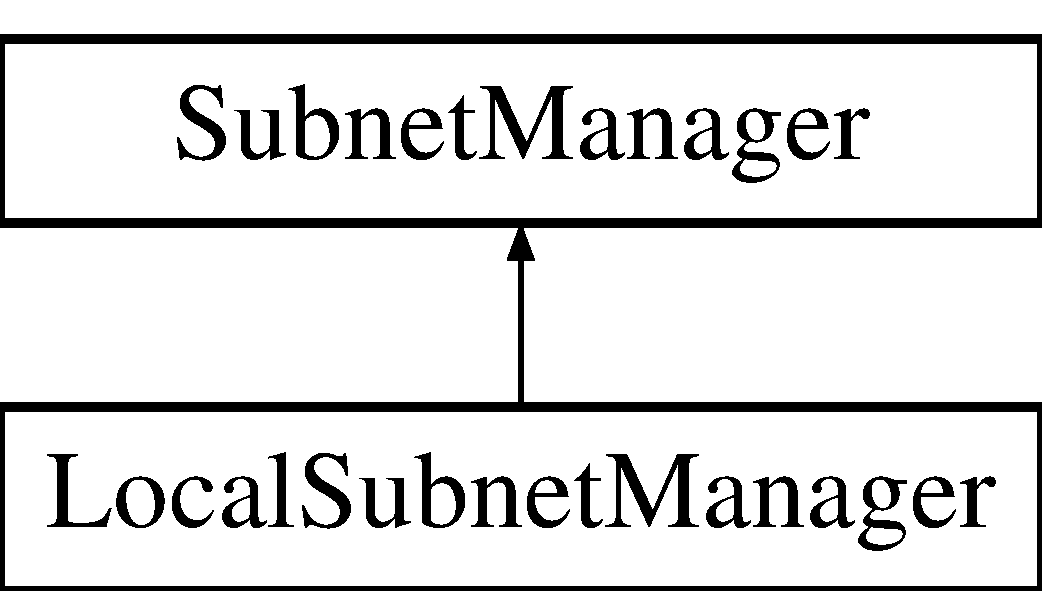
\includegraphics[height=2.000000cm]{classSubnetManager}
\end{center}
\end{figure}
\subsection*{Public Member Functions}
\begin{DoxyCompactItemize}
\item 
\mbox{\Hypertarget{classSubnetManager_af60bbdf2417a03b1e2fb14a5b077597a}\label{classSubnetManager_af60bbdf2417a03b1e2fb14a5b077597a}} 
{\bfseries Subnet\+Manager} (std\+::shared\+\_\+ptr$<$ \hyperlink{classSpaCommunicator}{Spa\+Communicator} $>$ com)
\item 
virtual void \hyperlink{classSubnetManager_a6aed1acaa5e9f18feb7667904675d119}{listen\+Messages} ()=0
\end{DoxyCompactItemize}
\subsection*{Static Protected Attributes}
\begin{DoxyCompactItemize}
\item 
static std\+::shared\+\_\+ptr$<$ \hyperlink{classSpaCommunicator}{Spa\+Communicator} $>$ \hyperlink{classSubnetManager_acb58a845a46fa4943cb2b9d4a56c9b0f}{communicator}
\begin{DoxyCompactList}\small\item\em Run a long running task on a new thread. \end{DoxyCompactList}\end{DoxyCompactItemize}


\subsection{Member Function Documentation}
\mbox{\Hypertarget{classSubnetManager_a6aed1acaa5e9f18feb7667904675d119}\label{classSubnetManager_a6aed1acaa5e9f18feb7667904675d119}} 
\index{Subnet\+Manager@{Subnet\+Manager}!listen\+Messages@{listen\+Messages}}
\index{listen\+Messages@{listen\+Messages}!Subnet\+Manager@{Subnet\+Manager}}
\subsubsection{\texorpdfstring{listen\+Messages()}{listenMessages()}}
{\footnotesize\ttfamily virtual void Subnet\+Manager\+::listen\+Messages (\begin{DoxyParamCaption}{ }\end{DoxyParamCaption})\hspace{0.3cm}{\ttfamily [pure virtual]}}


\begin{DoxyParams}{Parameters}
{\em message} & -\/ message that has been received Continuously ping components checking to make sure they are still responsive. Should report component failture to logging service. This function should not return while the subnet manager is running. Continuously listen for messages. Will call receive\+Message with each received message. A call to this method should not return while the subnet manager is running. \\
\hline
\end{DoxyParams}


Implemented in \hyperlink{classLocalSubnetManager_a8cd2838196edcd75a77f532bce15c2fd}{Local\+Subnet\+Manager}.



\subsection{Member Data Documentation}
\mbox{\Hypertarget{classSubnetManager_acb58a845a46fa4943cb2b9d4a56c9b0f}\label{classSubnetManager_acb58a845a46fa4943cb2b9d4a56c9b0f}} 
\index{Subnet\+Manager@{Subnet\+Manager}!communicator@{communicator}}
\index{communicator@{communicator}!Subnet\+Manager@{Subnet\+Manager}}
\subsubsection{\texorpdfstring{communicator}{communicator}}
{\footnotesize\ttfamily std\+::shared\+\_\+ptr$<$ \hyperlink{classSpaCommunicator}{Spa\+Communicator} $>$ Subnet\+Manager\+::communicator\hspace{0.3cm}{\ttfamily [static]}, {\ttfamily [protected]}}



Run a long running task on a new thread. 


\begin{DoxyParams}{Parameters}
{\em task} & -\/ lambda function to run on a seperate thread \\
\hline
\end{DoxyParams}


The documentation for this class was generated from the following files\+:\begin{DoxyCompactItemize}
\item 
lib/subnet\+\_\+manager.\+hpp\item 
lib/subnet\+\_\+manager.\+cpp\end{DoxyCompactItemize}

\hypertarget{structSubscriber}{}\section{Subscriber Struct Reference}
\label{structSubscriber}\index{Subscriber@{Subscriber}}
\subsection*{Public Member Functions}
\begin{DoxyCompactItemize}
\item 
\mbox{\Hypertarget{structSubscriber_a64dab4d8803d8814bf7a6e7162a2b436}\label{structSubscriber_a64dab4d8803d8814bf7a6e7162a2b436}} 
{\bfseries Subscriber} (\hyperlink{structLogicalAddress}{Logical\+Address} la, uint16\+\_\+t d)
\end{DoxyCompactItemize}
\subsection*{Public Attributes}
\begin{DoxyCompactItemize}
\item 
\mbox{\Hypertarget{structSubscriber_ad27b381f3d2a33920ff6664e4013abc3}\label{structSubscriber_ad27b381f3d2a33920ff6664e4013abc3}} 
\hyperlink{structLogicalAddress}{Logical\+Address} {\bfseries subscriber\+Address}
\item 
\mbox{\Hypertarget{structSubscriber_a8221a4d1ba53e0407b27e44cda4a87ab}\label{structSubscriber_a8221a4d1ba53e0407b27e44cda4a87ab}} 
uint16\+\_\+t {\bfseries delivery\+Rate\+Divisor}
\end{DoxyCompactItemize}


The documentation for this struct was generated from the following file\+:\begin{DoxyCompactItemize}
\item 
lib/component.\+hpp\end{DoxyCompactItemize}

\hypertarget{structSubscriptionReply}{}\section{Subscription\+Reply Struct Reference}
\label{structSubscriptionReply}\index{Subscription\+Reply@{Subscription\+Reply}}
\subsection*{Public Member Functions}
\begin{DoxyCompactItemize}
\item 
\mbox{\Hypertarget{structSubscriptionReply_a8b41ba60bc85ee15f7bddbaec3260ad0}\label{structSubscriptionReply_a8b41ba60bc85ee15f7bddbaec3260ad0}} 
{\bfseries Subscription\+Reply} (\hyperlink{structLogicalAddress}{Logical\+Address} destination, \hyperlink{structLogicalAddress}{Logical\+Address} source)
\item 
\mbox{\Hypertarget{structSubscriptionReply_a8e656028ab7b6750157b6d0ebbf06659}\label{structSubscriptionReply_a8e656028ab7b6750157b6d0ebbf06659}} 
{\bfseries Subscription\+Reply} (uint8\+\_\+t version, uint8\+\_\+t priority, uint16\+\_\+t length, \hyperlink{structLogicalAddress}{Logical\+Address} destination, \hyperlink{structLogicalAddress}{Logical\+Address} source, uint16\+\_\+t flags, uint16\+\_\+t dI, uint8\+\_\+t rT)
\end{DoxyCompactItemize}
\subsection*{Public Attributes}
\begin{DoxyCompactItemize}
\item 
\mbox{\Hypertarget{structSubscriptionReply_a4e4c24f7a85c8c2ac00604e9edf0bbab}\label{structSubscriptionReply_a4e4c24f7a85c8c2ac00604e9edf0bbab}} 
\hyperlink{structSpaMessage}{Spa\+Message} {\bfseries spa\+Message}
\item 
\mbox{\Hypertarget{structSubscriptionReply_a8fc1a335af866ee6e1328106421fee66}\label{structSubscriptionReply_a8fc1a335af866ee6e1328106421fee66}} 
uint16\+\_\+t {\bfseries dialog\+Id}
\item 
\mbox{\Hypertarget{structSubscriptionReply_a289965f913a0dac7204482b86798ed5a}\label{structSubscriptionReply_a289965f913a0dac7204482b86798ed5a}} 
uint8\+\_\+t {\bfseries reply\+Type}
\end{DoxyCompactItemize}


The documentation for this struct was generated from the following file\+:\begin{DoxyCompactItemize}
\item 
lib/messages/spa/subscription\+\_\+reply.\+h\end{DoxyCompactItemize}

\hypertarget{structSubscriptionRequest}{}\section{Subscription\+Request Struct Reference}
\label{structSubscriptionRequest}\index{Subscription\+Request@{Subscription\+Request}}


{\ttfamily \#include $<$subscription\+\_\+request.\+h$>$}

\subsection*{Public Member Functions}
\begin{DoxyCompactItemize}
\item 
\hyperlink{structSubscriptionRequest_a3b6895bbe1f616836913b7681b87a852}{Subscription\+Request} (\hyperlink{structLogicalAddress}{Logical\+Address} destination, \hyperlink{structLogicalAddress}{Logical\+Address} source, \hyperlink{structLogicalAddress}{Logical\+Address} mA)
\item 
\hyperlink{structSubscriptionRequest_a1fb7f2d417847d7df52ce23d00f632a6}{Subscription\+Request} (uint8\+\_\+t version, uint8\+\_\+t priority, \hyperlink{structLogicalAddress}{Logical\+Address} destination, \hyperlink{structLogicalAddress}{Logical\+Address} source, \hyperlink{structLogicalAddress}{Logical\+Address} mA, uint16\+\_\+t flags, uint32\+\_\+t lP, uint16\+\_\+t dI, uint16\+\_\+t d\+RD, uint8\+\_\+t iI, uint8\+\_\+t mI, uint8\+\_\+t sP, uint8\+\_\+t t)
\end{DoxyCompactItemize}
\subsection*{Public Attributes}
\begin{DoxyCompactItemize}
\item 
\hyperlink{structSpaMessage}{Spa\+Message} \hyperlink{structSubscriptionRequest_a33610286907a36d4ca8185a0208edcf8}{spa\+Message}
\item 
\hyperlink{structLogicalAddress}{Logical\+Address} \hyperlink{structSubscriptionRequest_af355bb5e7794b7c6613081982be6f72d}{producer\+Addr}
\item 
\hyperlink{structLogicalAddress}{Logical\+Address} \hyperlink{structSubscriptionRequest_ad686e1351ba99ca2a1ca4626f58bebac}{consumer\+Addr}
\item 
\hyperlink{structLogicalAddress}{Logical\+Address} \hyperlink{structSubscriptionRequest_a3b3f9db2899f3bec38a2d0c7ec8e6515}{manager\+Addr}
\item 
uint32\+\_\+t \hyperlink{structSubscriptionRequest_a3a7af51b8bf5ff34f09ed3599a19d0e1}{lease\+Period}
\item 
uint16\+\_\+t \hyperlink{structSubscriptionRequest_a7e6911856acf31c1367738e230524778}{dialog\+Id}
\item 
uint16\+\_\+t \hyperlink{structSubscriptionRequest_a85b4bd05a70308efe9dede88deef73de}{delivery\+Rate\+Divisor}
\item 
uint8\+\_\+t \hyperlink{structSubscriptionRequest_ab170a906e69ab9dbf8213a27e96276bd}{interface\+Id}
\item 
uint8\+\_\+t \hyperlink{structSubscriptionRequest_aee5c2ccd81b37daaad7d5aeeca12bdce}{message\+Id}
\item 
uint8\+\_\+t \hyperlink{structSubscriptionRequest_a5b8dd2c6614db580a69c675bc9016971}{subscription\+Priority}
\item 
uint8\+\_\+t \hyperlink{structSubscriptionRequest_a5603a9499051bd93fc94d729acb5785a}{type}
\end{DoxyCompactItemize}


\subsection{Constructor \& Destructor Documentation}
\mbox{\Hypertarget{structSubscriptionRequest_a3b6895bbe1f616836913b7681b87a852}\label{structSubscriptionRequest_a3b6895bbe1f616836913b7681b87a852}} 
\index{Subscription\+Request@{Subscription\+Request}!Subscription\+Request@{Subscription\+Request}}
\index{Subscription\+Request@{Subscription\+Request}!Subscription\+Request@{Subscription\+Request}}
\subsubsection{\texorpdfstring{Subscription\+Request()}{SubscriptionRequest()}\hspace{0.1cm}{\footnotesize\ttfamily [1/2]}}
{\footnotesize\ttfamily Subscription\+Request\+::\+Subscription\+Request (\begin{DoxyParamCaption}\item[{\hyperlink{structLogicalAddress}{Logical\+Address}}]{destination,  }\item[{\hyperlink{structLogicalAddress}{Logical\+Address}}]{source,  }\item[{\hyperlink{structLogicalAddress}{Logical\+Address}}]{mA }\end{DoxyParamCaption})\hspace{0.3cm}{\ttfamily [inline]}}

\mbox{\Hypertarget{structSubscriptionRequest_a1fb7f2d417847d7df52ce23d00f632a6}\label{structSubscriptionRequest_a1fb7f2d417847d7df52ce23d00f632a6}} 
\index{Subscription\+Request@{Subscription\+Request}!Subscription\+Request@{Subscription\+Request}}
\index{Subscription\+Request@{Subscription\+Request}!Subscription\+Request@{Subscription\+Request}}
\subsubsection{\texorpdfstring{Subscription\+Request()}{SubscriptionRequest()}\hspace{0.1cm}{\footnotesize\ttfamily [2/2]}}
{\footnotesize\ttfamily Subscription\+Request\+::\+Subscription\+Request (\begin{DoxyParamCaption}\item[{uint8\+\_\+t}]{version,  }\item[{uint8\+\_\+t}]{priority,  }\item[{\hyperlink{structLogicalAddress}{Logical\+Address}}]{destination,  }\item[{\hyperlink{structLogicalAddress}{Logical\+Address}}]{source,  }\item[{\hyperlink{structLogicalAddress}{Logical\+Address}}]{mA,  }\item[{uint16\+\_\+t}]{flags,  }\item[{uint32\+\_\+t}]{lP,  }\item[{uint16\+\_\+t}]{dI,  }\item[{uint16\+\_\+t}]{d\+RD,  }\item[{uint8\+\_\+t}]{iI,  }\item[{uint8\+\_\+t}]{mI,  }\item[{uint8\+\_\+t}]{sP,  }\item[{uint8\+\_\+t}]{t }\end{DoxyParamCaption})\hspace{0.3cm}{\ttfamily [inline]}}



\subsection{Member Data Documentation}
\mbox{\Hypertarget{structSubscriptionRequest_ad686e1351ba99ca2a1ca4626f58bebac}\label{structSubscriptionRequest_ad686e1351ba99ca2a1ca4626f58bebac}} 
\index{Subscription\+Request@{Subscription\+Request}!consumer\+Addr@{consumer\+Addr}}
\index{consumer\+Addr@{consumer\+Addr}!Subscription\+Request@{Subscription\+Request}}
\subsubsection{\texorpdfstring{consumer\+Addr}{consumerAddr}}
{\footnotesize\ttfamily \hyperlink{structLogicalAddress}{Logical\+Address} Subscription\+Request\+::consumer\+Addr}

\mbox{\Hypertarget{structSubscriptionRequest_a85b4bd05a70308efe9dede88deef73de}\label{structSubscriptionRequest_a85b4bd05a70308efe9dede88deef73de}} 
\index{Subscription\+Request@{Subscription\+Request}!delivery\+Rate\+Divisor@{delivery\+Rate\+Divisor}}
\index{delivery\+Rate\+Divisor@{delivery\+Rate\+Divisor}!Subscription\+Request@{Subscription\+Request}}
\subsubsection{\texorpdfstring{delivery\+Rate\+Divisor}{deliveryRateDivisor}}
{\footnotesize\ttfamily uint16\+\_\+t Subscription\+Request\+::delivery\+Rate\+Divisor}

\mbox{\Hypertarget{structSubscriptionRequest_a7e6911856acf31c1367738e230524778}\label{structSubscriptionRequest_a7e6911856acf31c1367738e230524778}} 
\index{Subscription\+Request@{Subscription\+Request}!dialog\+Id@{dialog\+Id}}
\index{dialog\+Id@{dialog\+Id}!Subscription\+Request@{Subscription\+Request}}
\subsubsection{\texorpdfstring{dialog\+Id}{dialogId}}
{\footnotesize\ttfamily uint16\+\_\+t Subscription\+Request\+::dialog\+Id}

\mbox{\Hypertarget{structSubscriptionRequest_ab170a906e69ab9dbf8213a27e96276bd}\label{structSubscriptionRequest_ab170a906e69ab9dbf8213a27e96276bd}} 
\index{Subscription\+Request@{Subscription\+Request}!interface\+Id@{interface\+Id}}
\index{interface\+Id@{interface\+Id}!Subscription\+Request@{Subscription\+Request}}
\subsubsection{\texorpdfstring{interface\+Id}{interfaceId}}
{\footnotesize\ttfamily uint8\+\_\+t Subscription\+Request\+::interface\+Id}

\mbox{\Hypertarget{structSubscriptionRequest_a3a7af51b8bf5ff34f09ed3599a19d0e1}\label{structSubscriptionRequest_a3a7af51b8bf5ff34f09ed3599a19d0e1}} 
\index{Subscription\+Request@{Subscription\+Request}!lease\+Period@{lease\+Period}}
\index{lease\+Period@{lease\+Period}!Subscription\+Request@{Subscription\+Request}}
\subsubsection{\texorpdfstring{lease\+Period}{leasePeriod}}
{\footnotesize\ttfamily uint32\+\_\+t Subscription\+Request\+::lease\+Period}

\mbox{\Hypertarget{structSubscriptionRequest_a3b3f9db2899f3bec38a2d0c7ec8e6515}\label{structSubscriptionRequest_a3b3f9db2899f3bec38a2d0c7ec8e6515}} 
\index{Subscription\+Request@{Subscription\+Request}!manager\+Addr@{manager\+Addr}}
\index{manager\+Addr@{manager\+Addr}!Subscription\+Request@{Subscription\+Request}}
\subsubsection{\texorpdfstring{manager\+Addr}{managerAddr}}
{\footnotesize\ttfamily \hyperlink{structLogicalAddress}{Logical\+Address} Subscription\+Request\+::manager\+Addr}

\mbox{\Hypertarget{structSubscriptionRequest_aee5c2ccd81b37daaad7d5aeeca12bdce}\label{structSubscriptionRequest_aee5c2ccd81b37daaad7d5aeeca12bdce}} 
\index{Subscription\+Request@{Subscription\+Request}!message\+Id@{message\+Id}}
\index{message\+Id@{message\+Id}!Subscription\+Request@{Subscription\+Request}}
\subsubsection{\texorpdfstring{message\+Id}{messageId}}
{\footnotesize\ttfamily uint8\+\_\+t Subscription\+Request\+::message\+Id}

\mbox{\Hypertarget{structSubscriptionRequest_af355bb5e7794b7c6613081982be6f72d}\label{structSubscriptionRequest_af355bb5e7794b7c6613081982be6f72d}} 
\index{Subscription\+Request@{Subscription\+Request}!producer\+Addr@{producer\+Addr}}
\index{producer\+Addr@{producer\+Addr}!Subscription\+Request@{Subscription\+Request}}
\subsubsection{\texorpdfstring{producer\+Addr}{producerAddr}}
{\footnotesize\ttfamily \hyperlink{structLogicalAddress}{Logical\+Address} Subscription\+Request\+::producer\+Addr}

\mbox{\Hypertarget{structSubscriptionRequest_a33610286907a36d4ca8185a0208edcf8}\label{structSubscriptionRequest_a33610286907a36d4ca8185a0208edcf8}} 
\index{Subscription\+Request@{Subscription\+Request}!spa\+Message@{spa\+Message}}
\index{spa\+Message@{spa\+Message}!Subscription\+Request@{Subscription\+Request}}
\subsubsection{\texorpdfstring{spa\+Message}{spaMessage}}
{\footnotesize\ttfamily \hyperlink{structSpaMessage}{Spa\+Message} Subscription\+Request\+::spa\+Message}

\mbox{\Hypertarget{structSubscriptionRequest_a5b8dd2c6614db580a69c675bc9016971}\label{structSubscriptionRequest_a5b8dd2c6614db580a69c675bc9016971}} 
\index{Subscription\+Request@{Subscription\+Request}!subscription\+Priority@{subscription\+Priority}}
\index{subscription\+Priority@{subscription\+Priority}!Subscription\+Request@{Subscription\+Request}}
\subsubsection{\texorpdfstring{subscription\+Priority}{subscriptionPriority}}
{\footnotesize\ttfamily uint8\+\_\+t Subscription\+Request\+::subscription\+Priority}

\mbox{\Hypertarget{structSubscriptionRequest_a5603a9499051bd93fc94d729acb5785a}\label{structSubscriptionRequest_a5603a9499051bd93fc94d729acb5785a}} 
\index{Subscription\+Request@{Subscription\+Request}!type@{type}}
\index{type@{type}!Subscription\+Request@{Subscription\+Request}}
\subsubsection{\texorpdfstring{type}{type}}
{\footnotesize\ttfamily uint8\+\_\+t Subscription\+Request\+::type}



The documentation for this struct was generated from the following file\+:\begin{DoxyCompactItemize}
\item 
lib/messages/spa/\hyperlink{subscription__request_8h}{subscription\+\_\+request.\+h}\end{DoxyCompactItemize}

%--- End generated contents ---

% Index
\backmatter
\newpage
\phantomsection
\clearemptydoublepage
\addcontentsline{toc}{chapter}{Index}
\printindex

\end{document}
